
%%%%%%%%%%%%%% Document class
%%%\documentclass[a4paper,BCOR1.5cm,twoside,DIV12]{scrbook}
%\documentclass[a4paper,11pt,oneside,DIV15]{scrbook}
%\documentclass[a4paper,11pt,oneside,DIV15]{scrartcl}

% Sele��o do tipo de monografia e das op��es de formata��o
\documentclass[openright,diss]{deletex}

% um tipo espec�fico de monografia pode ser informado como par�metro opcional:
%\documentclass[tese]{deletex}

% O tipo de monografia pode ser:
% diss 			disserta��o de mestrado
% rp 			relat�rio de pesquisa
% prop-tese 		proposta de tese de doutorado
% plano-doutorado 	plano de curso de doutorado
% dipl-ele 		projeto de diploma��o em Engenharia El�trica
% dipl-ecp		projeto de diploca��o em Engenharia de Computa��o
% estagio		relat�rio de est�gio supervisionado 
% ti			trabalho individual
% pep			plano de estudos e pesquisa
% tese			tese de doutorado
% tc			trabalho de conclus�o de mestrado profissional
% espec			monografia de conclus�o de curso de especializa��o

% � importante notar que estes tipos de monografia foram herdados do estilo
% do II/UFRGS e n�o necessariamente aplicam-se ao DELET/EE/UFRGS. Ou seja,
% embora a classe deletex.cls defina uma opcao para elaborar um PEP, isto nao
% significa que um PEP seja exigido pelo PPGEE.

% monografias em ingl�s devem receber o par�metro `english':
%\documentclass[diss,english]{deletex}

% a op��o `openright' pode ser usada para for�ar in�cios de cap�tulos
% em p�ginas �mpares
% \documentclass[openright]{deletex}

% para gerar uma vers�o somente-frente, basta utilizar a op��o `oneside':
% \documentclass[oneside]{deletex}

% A opcao numbers pode ser usada para gerar refer�ncia num�ricas.
% A opcao sort&compress faz com que referencias do tipo [8,5,3,4] sejam
% convertidas para [3-4,8]
%\documentclass[numbers,sort&compress]{deletex}

% A opcao relnum faz com que a numeracao de figuras, tabelas e equa��es
% seja por cap�tulo.
%\documentclass[relnum]{deletex}


%%%%%%%%%%%%%%%%%%%%%%%%%%%%%%%%%%%%%%%%%%%%%%%%%%%%%%%%%%%%%%%%%%%%%%%%%%%%%%%%%%%%%%%%%%%%%%%%%%%%%%%%
% Preambule
\usepackage[latin1]{inputenc}   % Zeichensatz
\usepackage{graphicx}           % Einbinden von Grafiken
\usepackage{verbatim}
\usepackage{alltt}              % Verbatim-Umgebung mit Steuerbefehlen (z.B. fett, kursiv, ...)
\usepackage{booktabs}           % Paket f�r sch�nere Tabellen
\usepackage{subfigure}
\usepackage{url}
\usepackage{ae}
\usepackage{float}
\usepackage{psfrag}
\usepackage{amsfonts}
\usepackage{amssymb}
\usepackage{amsmath}
\usepackage{pstricks,pst-node,pst-text,pst-3d}
%\usepackage{hyperref}   % use for hypertext links, including those to external documents and URLs
%\usepackage[breaklinks=true]{hyperref}
%\usepackage[brazil]{babel} %get everything translated properly
\usepackage[brazilian]{babel} %get everything translated properly
%\selectlanguage{brazil}
%\usepackage[numbers]{natbib}
\usepackage{enumerate}
%\usepackage{newclude}

\usepackage{listings}           % Paket, um Listings sch�n einbinden zu k�nnen
\lstloadlanguages{Matlab}
%\usepackage[usenames,dvipsnames]{color}
%\usepackage{thumbpdf}           % Thumbnails f�r Seitenvorschau
%\usepackage{algorithm}
%\usepackage{algorithmicx}
%\usepackage{algpseudocode}
%\usepackage[portuguese,onelanguage,ruled,noline,linesnumbered]{algorithm2e}
%\usepackage[portuguese,ruled,noline]{algorithm2e}

%\usepackage{amsmath}
\usepackage{amsthm}
%\usepackage{amsfonts}
%\usepackage{amssymb}
%\usepackage{thmtools}
%\declaretheoremstyle[,
%bodyfont=\normalfont
%]{mystyle}
%\declaretheorem[name=Exemplo,style=mystyle,numberwithin=chapter]{example}
%\declaretheorem[name=Exemplo,numberwithin=section]{example}
%\usepackage{balance}
%\usepackage{setspace}
%
%\usepackage{multirow}
%\usepackage{rotating}
%
%\usepackage{subfig}
%\usepackage{fancyhdr}
%\usepackage{layout}
%\usepackage{chngpage}
%\usepackage{colortbl}
%\usepackage{float}
%\usepackage[intoc,noprefix]{nomencl}
\usepackage{tikz}
\usetikzlibrary{shapes,arrows}

%%\renewcommand{\nomname}{List of Symbols}

%\makenomenclature

%\usepackage{losymbol}

%%%\usepackage{makeidx}            % F�r Benutzung des Befehls \printindex
%%%\usepackage{flafter}            % Platziert Gleitobjekte nach ihrer Definition

%%%\usepackage{german}            % Erm�glich die direkte Eingabe von Umlauten
%%%\usepackage{bibgerm}           % Bitex: Deutscher Style der Literaturreferenzen
%\usepackage{caption}           % �berschriften f�r floating Umgebungen, %%z.B. f�r Tabellen und Bilder
%%%\usepackage{pslatex,times}     % Setzt die Schriftart Times als Standardschriftart
%%%\usepackage{nomencl}           % Legt eine Liste aller Symboldefinitionen (z.B. �P = ...) an
%%%\usepackage{textcomp}          % Zus�tzliche mathematische Symbole
%%%\usepackage{amssymb}           % Americam mathematican Society -> Symbole


%\usepackage{amsfonts}% to get the \mathbb alphabet
%\newcommand{\field}[1]{\mathbb{#1}}
%\newcommand{\setc}[1]{\mathcal{#1}}
%\newcommand{\C}{\field{C}}
%\newcommand{\R}{\field{R}}
%\newcommand{\vect}{\mathbf}
%\newcommand{\matr}{\mathbf}
%\renewcommand\Re{\operatorname{Re}}
%\renewcommand\Im{\operatorname{Im}}
%\newcommand{\pderfrac}[2]{\frac{\partial#1}{\partial#2}}
%\providecommand{\trans}[1]{{#1}^\mathrm{T}}

%\hhhypersetup{
%	colorlinks,
%	debug=true,
%	linkcolor=black,  %%% cor do tableofcontents, \ref, \footnote, etc
%	citecolor=red,  %%% cor do \cite
%	urlcolor=blue,   %%% cor do \url e \href
%	bookmarksopen=true,
%	pdftitle={Disserta��o de Mestrado},
%	pdfauthor={Tassiano Neuhaus},
%	pdfsubject={Projeto de controladores n�o lineares representados por modelos NARMAX usando refer�ncia virtual.},
%	pdfkeywords={System identification, data-base control design, Virttual Reference, nonlinear systems, NARMAX models},
%	%pdfpagemode=FullScreen
%}

%%%%%%%%%%%%%%%%%%%%%%%%%%%%%%%%%%%%%%%%%%%%%%%%%%%%%%%%%%%%%%%%%%%%%%%%%%%%%%%%%%%%%%%%%%%%%%%%%%%%%%%%%

% Setings for Code Listing
\lstset{
	language=VHDL,
	frame=single,
	commentstyle=\footnotesize,
	basicstyle=\footnotesize\ttfamily,
	%basicstyle=\small\ttfamily,%
	tabsize=1,%
	keywordstyle=\color{blue}\bfseries,%
	captionpos=b,  % caption position: bottom
	showstringspaces=false,
	numbers=left,%
	numberstyle=\footnotesize,
	%stepnumber=2,               % Abstand zwischen den Zeilennummern
	numbersep=1pt,              % Abstand der Nummern zum Text
	framexleftmargin=6mm,
	framexrightmargin=-6mm,%
	xleftmargin=6mm,
	xrightmargin=10mm,
	breaklines=true
	escapechar=$
}

\usepackage{pdflscape}

\usepackage{geometry}
\geometry{hcentering}
%%\geometry{a4paper,textwidth=153mm,textheight=224mm,top=35mm,hcentering}

%%%% Some self made macros


%%%%%%%%%%%%%%%%%%%%%%%%%%%%
%-+
%+ \TODO[<wer>]{<text>}
%+-
%- Erzeugt am Seitenrand den <text> mit dem zus�tzlichen
%- Vermerk, f�r <wen> dieses TODO noch offen ist.
%-
\newcommand{\TODO}[2][ICH]{%
\marginpar{\footnotesize \color{red} TODO [#1]:\\%
#2}}

%%%%%%%%%%%%%%%%%%%%%%%%%%%%
%
% \todobf{text}
%
\newcommand{\todobf}[1]{{\color{red}\textbf{TODO:  #1}}}


%%%%%%%%%%%%%%%%%%%%%%%%%%%%
%
% \note{text}
%
\newcommand{\note}[1]{{\color{red}\rule{0.5em}{1ex} \textbf{#1}}}

%%%%%%%%%%%%%%%%%%%%%%%%%%%%
%
% \tred{text}
%
\newcommand{\tred}[1]{{\textcolor{red}{#1}}}

%%%%%%%%%%%%%%%%%%%%%%%%%%%%
%
% Change the standard name "Bibliography" to "References", which is required by ABNT
%
\renewcommand\bibname{References}



%\newcounter{example}[chapter]
%\newenvironment{example}{\refstepcounter{example}
%  \subsubsection{Exemplo
%    \thechapter.\arabic{example}}}{\\}
%  %%\thechapter.\arabic{example}}\em}{\\}  %% O \em define o estilo da fonte utilizada no ambiente exemplo
%
%\renewcommand{\theexample}{\thechapter.\arabic{example}}










%%% Choosing arabic numbers for paging
%\pagenumbering{arabic}
%
%
%\begin{comment}
%%%% Setting Headers and Footers
%\pagestyle{fancy}
%\fancyhead{}
%\fancyfoot{}
%\fancyhead[RE]{\slshape \leftmark}
%\fancyhead[LE,RO]{\thepage}
%\fancyhead[LO]{\slshape \rightmark}
%%\renewcommand{\headrulewidth}{0.4pt}
%%%\renewcommand{\footrulewidth}{0.4pt}
%\end{comment}

%%%% For the Paragraph indentationa and distance
%\parindent 0pt
%\parskip 1.5ex

\newtheorem{theorem}{Teorema}[chapter]
\newtheorem{lemma}{Lemma}[chapter]
\newtheorem{prop}[theorem]{Proposi��o}
\newtheorem{cor}[theorem]{Corol�rio}
\newtheorem{defn}[theorem]{Defini��o}

\tikzstyle{block} = [draw, fill=blue!20, rectangle, minimum height=3em, minimum width=6em]
\tikzstyle{sum} = [draw, fill=blue!20, circle, node distance=1cm]
\tikzstyle{input} = [coordinate]
\tikzstyle{output} = [coordinate]
\tikzstyle{pinstyle} = [pin edge={to-,thin,black}]


% Informa��es gerais
%
\title{Um Exemplo de Disserta��o (Monografia, Tese, Projeto de Diploma��o,
		Relat�rio de Est�gio Supervisionado, Etc.) Apresentada ao PPGEE ou ao
	DELET}

\author{Flaumann}{Fritz Gutenberg}
% alguns documentos podem ter varios autores:
%\author{Flaumann}{Frida Gutenberg}
%\author{Flaumann}{Klaus Gutenberg}

% orientador
\advisor[Prof.~Dr.]{Lamport}{Leslie}
\advisorinfo{Microsoft}{Doutor pela Brandeis University -- Waltham, EUA}

% O comando \advisorwidth pode ser usado para ajustar o tamanho do campo
% destinado ao nome do orientador, de forma a evitar que ocupe mais de uma linha 
%\advisorwidth{0.55\textwidth}

% obviamente, o co-orientador � opcional
%\coadvisor[Prof.~Dr.]{Knuth}{Donald E.}
\coadvisorinfo{Stanford}{Doutor pelo California Institute of Technology -- Pasadena, EUA}

% banca examinadora
\examiner[Prof.~Dr.]{Goossens}{Michel}
\examinerinfo{CERN}{Doutor pela Vrije Universiteit Brussel -- Bruxelas, B�lgica}
\examiner[Prof.~Dr.]{Gomes da Silva Jr.}{Jo�o Manuel}
\examinerinfo{UFRGS}{Doutor pela Universit� Paul Sabatier -- Toulouse, Fran�a}
\examiner[Prof.~Dr.]{Carro}{Luigi}
\examinerinfo{UFRGS}{Doutor pela Universidade Federal do Rio Grande do Sul -- Porto Alegre, Brasil}

% a data deve ser a da defesa; se nao especificada, s�o gerados
% mes e ano correntes
%\date{fevereiro}{2004}

% o nome do curso pode ser redefinido (ex. para Monografias)
%\course{Curso de Qualquer Coisa}

% o nome da disciplina pode ser definido
%\subject{ENG04006 Sistemas e Sinais}

% o local de realiza��o do trabalho pode ser especificado (ex. para Monografias)
% com o comando \location:
%\location{S�o Jos� dos Campos}{SP}

% itens individuais da nominata podem ser redefinidos com os comandos
% abaixo:
% \renewcommand{\nominataReit}{Prof\textsuperscript{a}.~Dr.~Jos{\'e} Carlos Ferraz Hennemann}
% \renewcommand{\nominataReitname}{Reitor}
% \renewcommand{\nominataPRE}{Prof.~Dr.~Pedro Cezar Dutra Fonseca}
% \renewcommand{\nominataPREname}{Pr{\'o}-Reitor de Ensino}
% \renewcommand{\nominataPRAPG}{Prof\textsuperscript{a}.~Dr\textsuperscript{a}.~Valqu\'{\i}ria Linck Bassani}
% \renewcommand{\nominataPRAPGname}{Pr{\'o}-Reitora de P{\'o}s-Gradua{\c{c}}{\~a}o}
% \renewcommand{\nominataDir}{Prof.~Dr.~Alberto Tamagna}
% \renewcommand{\nominataDirname}{Diretor da Escola de Engenharia}
% \renewcommand{\nominataCoord}{Prof.~Dr.~Marcelo Soares Lubaszewski}
% \renewcommand{\nominataCoordname}{Coordenador do PPGEE}
% \renewcommand{\nominataBibchefe}{June Magda Rosa Schamberg}
% \renewcommand{\nominataBibchefename}{Bibliotec{\'a}ria-chefe da Escola de Engenharia}
% \renewcommand{\nominataChefeDELET}{Prof.~Dr.~Romeu Reginatto}
% \renewcommand{\nominataChefeDELETname}{Chefe do \delet}

% A seguir s�o apresentados comandos espec�ficos para alguns
% tipos de documentos.

% Tese de doutorado [tese] e disserta��o de mestrado [diss]:
\topic{\ca}	% area de concentracao, uma entre:
			% \ca Controle e Automa��o
			% \tic Tecnologia de Informa��o e comunica��es
			% \se Sistemas de Energia

% Relat�rio de Pesquisa [rp]:
% \rp{123}             % numero do rp
% \financ{CNPq, CAPES} % orgaos financiadores

% Trabalho Individual [ti]:
% \ti{123}     % numero do TI
% \ti[II]{456} % no caso de ser o segundo TI

% Monografias de Especializa��o [espec]:
% \topic{Automa��o Industrial}      % nome do curso
% \coord[Prof.]{Bazanella}{Alexandre Sanfelice} % coordenador do curso
% \dept{DELET}                                 % departamento relacionado

% Projeto de diploma��o em Engenharia El�trica [dipl-ele] ou em Engenharia
% de Computa��o [dipl-ecp]:
% Pode-se definir explicitamente o nome do curso (\course):
%\course{\cgele}
%\course{\cgecp}
%\course{\cgeca}
%
% palavras-chave
% iniciar todas com letras min�sculas, exceto no caso de abreviaturas
%
\keyword{formata��o eletr�nica de documentos}
\keyword{\LaTeX}
\keyword{ABNT}
\keyword{UFRGS}




\begin{document}

% O comando \maketile gera a capa, a folha de rosto e a folha de aprovacao 
% (se for o caso)
% �s vezes � necess�rio redefinir algum comando logo antes de produzir
% a Capa, folha de rosto e folha de aprovacao:
% \renewcommand{\coordname}{Coordenadora do Curso}
\maketitle

% dedicatoria � opcional
\chapter*{Dedicat�ria}
Dedico aos dedicados.

% agradecimentos s�o opcionais
\chapter*{Agradecimentos}
Agrade�o ao \LaTeX\ por n�o ter v�rus de macro\ldots



% resumo no idioma do documento
\begin{abstract}
Este documento � um exemplo de como formatar documentos para o
Departamento de Engenharia El�trica da UFRGS usando a classe \LaTeX\
{\tt deletex.cls}. Ao mesmo tempo, pode servir de consulta
para comandos mais gen�ricos. \emph{O texto do resumo n�o deve
conter mais do que 500 palavras.}
\end{abstract}

% resumo no outro idioma
% como parametro devem ser passadas as palavras-chave
% no outro idioma, separadas por v�rgulas
\begin{englishabstract}{Electronic document preparation, \LaTeX, ABNT, UFRGS}
This document is an example on how to prepare documents at DELET/EE/UFRGS
using the \LaTeX\ class {\tt deletex.cls}. At the same time, it
may serve as a guide for general-purpose commands. \emph{The text in
the abstract should not contain more than 500~words.}
\end{englishabstract}

% Conforme a NBR 6027, secao 4, o sum�rio deve ser o �ltimo elemento pr�-textual. O
% modelo do PPGEE nao atende a esta exigencia. Obviamente, a norma deve ter a
% preced�ncia.




% lista de ilustra��es
\listoffigures

% lista de tabelas
\listoftables

% lista de abreviaturas e siglas em ordem alfab�tica
% o par�metro deve ser a abreviatura mais longa
\begin{listofabbrv}{NARMAX}
	\item[LTI] Linear time invariant
	\item[SISO] Single input single output
	\item[ARX] Auto regressive witg exogenous input
	\item[ARMAX] Auto regressive moving average with exogenous input]
	\item[NARMAX] Nonlinear autoregressive moving average model with exogenous variables
	\item[NARX] nonlinear autoregressive model with exogenous variables
	\item[RBF] Radial basis functions
	\item[BJ] Box-Jenkins
	\item[OE] Output Error
	\item[VRFT] Virtual Reference Feedback Tuning
	\item[MMQ] M�todo dos m�nimos quadrados
	\item[LMI] Linear Matrix Inequality
	\item[PRBS] Pseudo randon binary sequence
	\item[CC] Corrente continua
	\item[FDT] Frequency domain Tuning
	\item[CbT] Correlation-based Tuning
	\item[IFT] Iterative feedback tuning
	\item[PI] Proporcional Integral
	\item[PID] Proporcional Integral Derivativo
\end{listofabbrv}

% lista de s�mbolos em ordem alfab�tica (opcional)
\begin{listofsymbols}{$H(q, \theta)$}
	\item [$G_0(z)$] Fun��o de transfer�ncia que representa a planta real do sistema.
	\item [$G(q, \theta)$] Fun��o de transfer�ncia que representa a planta a ser estimada na identifica��o.
	\item [$H_0(z)$] Fun��o de transfer�ncia desconhecida que altera o ru�do branco que atua sobre o sistema.
	\item [$H(q, \theta)$] Fun��o de transfer�ncia que altera o ru�do branco que atua sobre o sistema, a qual se quer
	identificar.
	\item [$\theta^*$] Representa o conjunto de par�metros que faz com que o modelo identificado seja igual ao sistema
	real.
	\item [$\theta$] representa um conjunto de par�metros estimado do sistema.
	\item [$\hat{\theta}_N$] representa a estimativa para um certo valor de N pontos.
	\item [$\mathcal{S}$] Representa o sistema real sob an�lise.
	\item [$\mathcal{M}$] representa a classe de modelos utilizada para identificar o sistema real.
	\item [$T(z)$] representa o comportamento do sistema em malha fechada.
	\item [$T_d(z)$] representa o comportamento do sistema em malha fechada desejado.
	\item [$u(t)$] Sinal de sa�da do controlador ou entrada da planta.
	\item [$y(t)$] sinal de sa�da da planta.
	\item [$e(t)$] Ruido branco.
	\item [$\nu(t)$] ru�do resultante depois que o ru�dio branco � alterado por $H_0(z)$
	\item [$\phi$] vari�vel de regress�o utilizada para identifica��o do sistema.
	\item [$Z(t)$] instrumento utilizado no m�todo de vari�veis instrumentais.
	\item [$E(\cdot)$] representa a esperan�a de valor.
	\item [$\Phi$ ] representa o espectro de um sinal.
	\item [$\prod$] Produt�rio
	\item [$\sum$] Somat�rio
	\item [$L(z)$] Filtro utilizado no m�todo VRFT.
	\item [$\sigma_e^2$] Vari�ncia do ru�do.
	\item [$\chi^2$] Nivel de confian�a 
\end{listofsymbols}

% Conforme a NBR 6027, secao 4, o sum�rio deve ser o �ltimo elemento
% pr�-textual. O modelo do PPGEE nao atende a esta exigencia. Obviamente, a
% norma deve ter a preced�ncia.

% sumario
\tableofcontents





% AQUI COME�A O TEXTO PROPRIAMENTE DITO
% e aqui vai a parte principal
%
%===============================================================================
\chapter{Introdu��o}
\label{chapter:intro}
%===============================================================================

A teoria de identifica��o de sistemas � foco de estudo h� diversas d�cadas por in�meros engenheiros e pesquisadores em
diversas �reas. Muitas aplica��es existentes se baseiam direta ou indiretamente no uso de identifica��o de sistemas e
muitas outras aplica��es est�o em processo de desenvolvimento. Dentro deste contexto, o estudo da teoria de
identifica��o de sistemas � muito vasto e neste trabalho tem-se o interesse em apresentar alguns pontos relativos a
este assunto que s�o base para o desenvolvimento deste trabalho.

Basicamente a identifica��o de um sistema, ou uma parte de um sistema maior, pode ser dividido em tr�s componentes
principais: � necess�rio que exista um sistema real; uma classe de modelos, que pretende representar este sistema real;
um crit�rio que elenca, dentre os infinitos modelos que podem ser obtidos a partir de uma classe, qual � o que melhor
representa este sistema. Do sistema real coletam-se os dados que ser�o utilizados para  proceder o
processo de identifica��o, e muitas das propriedades das estimativas obtidas s�o baseadas na qualidade e quantidade das
informa��es que estes dados coletados conseguem trazer do sistema real.

Nesta quest�o de informatividade existe uma grande e vasta quantidade de pesquisa desenvolvida e em desenvolvimento.
Quest�es como projetos de experimentos que neste trabalho s�o abordados superficialmente e que para a identifica��o de
sistemas s�o uma ferramenta formid�vel, possuem aplicabilidade em diversas �reas. Em engenharia, a escolha do sinal
que ser� utilizado para excitar o sistema pode, entre outras caracter�sticas, reduzir erros da estimativa, reduzir tempo
e custo do processo de identifica��o, aumentar a confiabilidade das estimativas obtidas.

Entretanto n�o � apenas o sinal de entrada do sistema que determina as propriedades estat�sticas dos experimentos de
identifica��o executados. A escolha da classe de modelos para identificar o sistema � de crucial import�ncia para
que haja sucesso no processo de identifica��o. A escolha desta classe deve ser tomada com base em diversas
diretrizes, o que torna sua escolha outro foco extremamente diversificado de estudo para a teoria de identifica��o de sistemas.

Observa-se com certa frequ�ncia que uma classe de modelos � mais perform�tica para representar certos tipos de sistemas.
Isso � devido ao fato de que as classes de modelos ou estruturas de modelos se diferenciam umas das outras devido ao uso
de bases diferentes para representar cada sistema. Desta forma, sistemas que possuem uma afinidade maior com certas
bases s�o representados com um n�mero menor de par�metros do que quando uma base qualquer � utilizada. A busca por uma
classe de modelos simples, mas que ainda assim consiga representar o sistema real � tamb�m foco de diversos estudos. A
identifica��o de um sistema que n�o possua um n�mero desnecess�rio de par�metros � sempre almejado, desta forma reduz-se
a possibilidade de exist�ncia de din�micas no modelo que n�o est�o presentes no processo real, al�m de reduzir a
complexidade dos algoritmos utilizados na identifica��o.

Em se tratando de aplica��es na �rea da engenharia, o controle de sistemas tem um destaque especial no uso da teoria de
identifica��o de sistemas para a obten��o dos par�metros do controlador desejado. Muitos dos projetos de controladores
baseados em dados se utilizam desta teoria para firmar suas bases e determinar seu funcionamento.

Assim como identifica��o de sistemas, projetos de controladores baseados em dados s�o foco de estudo em v�rias e diversas
linhas de pesquisa h� d�cadas. Neste trabalho ser� dado enfoque ao uso de refer�ncia virtual para a obten��o
dos sinais necess�rios para a identifica��o do controlador. Refer�ncia virtual � largamente utilizada
pelo m�todo VRFT que, por ser um m�todo direto, n�o requer que haja um conhecimento do modelo da planta para que o
controlador possa ser projetado. Este m�todo prop�e-se a encontrar o controlador �timo com apenas um conjunto de dados
proveniente do sistema. 

Estas caracter�sticas s�o bastante atrativas para diversas aplica��es, sobretudo �quelas onde a parada do processo para
execu��o de testes e experimentos � indesejada, ou por vezes, invi�vel. Entretanto o uso do m�todo VRFT possui algumas
limita��es, a maioria deles j� apontadas em diversos trabalhos. Contudo, o uso deste m�todo para sistemas
n�o lineares � ainda bastante incipiente e os trabalhos existentes nesta �rea exigem que haja um consider�vel conhecimento da planta e
do sinal aplicado para que as estimativas sejam realizadas com margens de erro conhecidas.

O trabalho aqui apresentado tem por objetivo endere�ar uma parte deste problema. Para isso usou-se a ideia de
refer�ncia virtual utilizada pelo m�todo VRFT para determinar quais s�o os sinais necess�rios para identificar o
controlador ideal, que leva o sistema a se comportar em malha fechada como especificado. De posse destes sinais obtidos
de forma virtual al�m daqueles medidos diretamente do sistema, utilizam-se estas informa��es para alimentar um
algoritmo de identifica��o de sistemas n�o lineares. Neste contexto, o sistema n�o linear que se quer identificar � o
controlador que atuar� sobre a planta.

Para limitar o escopo do trabalho desenvolvido aqui, algumas decis�es sobre estrutura de modelos foram tomadas: optou-se
pela identifica��o de controladores n�o lineares que s�o representados por modelos NARMAX.

Para demonstrar o funcionamento desta proposta de identifica��o de controladores n�o lineares, diversos exemplos ser�o
abordados, tanto do algoritmo implementado quanto para o conjunto do uso de refer�ncia virtual e classes de modelos NARMAX.
Os exemplos abordados t�m o intuito de apresentar propriedades das estimativas e avaliar o desempenho da proposta em
atingir seus objetivos.

Este trabalho tem a seguinte organiza��o: no Cap�tulo \ref{chapter:system_identification} ser�o abordados assuntos b�sicos
da teoria de identifica��o de sistemas. Quest�es como a escolha da classe de modelos, do m�todo de identifica��o, das
propriedades estat�sticas que as estimativas obtidas possuem e uma breve introdu��o ao que � conhecido como projeto de
experimentos para determinar a escolha de sinais de entrada e de objetivos de identifica��o. No Cap�tulo
\ref{chapter:nlin_si_ident} s�o introduzidas algumas caracter�sticas de sistemas n�o lineares. S�o apresentadas as
classes de modelos mais comumente utilizadas para descri��o destes sistemas. Neste cap�tulo tamb�m � apresentado o algoritmo de
identifica��o de modelos NARMAX tanto racionais como polinomiais e alguns exemplos de uso.

No Cap�tulo \ref{chapter:dbcd} s�o introduzidos alguns conceitos sobre projeto de controladores baseados em dados.
Apresentam-se brevemente alguns dos principais m�todos conhecidos e estende-se a discuss�o para apresentar o m�todo VRFT
e com ele a ideia de refer�ncia virtual. S�o tamb�m apresentados neste cap�tulo alguns exemplos de uso do m�todo VRFT e
suas propriedades para situa��es onde o sistema � corrompido por ru�do ou quando a classe de modelos n�o consegue
representar o controlador ideal desejado.

No Cap�tulo \ref{chapter:dbnarmax} s�o apresentadas as contribui��es deste trabalho com a uni�o de refer�ncia virtual e
o algoritmo de identifica��o de sistemas n�o lineares que podem ser descritos por classes de modelos NARMAX. S�o
apresentados exemplos de uso para sistemas onde a n�o linearidade est� na din�mica do processo e quando est� acoplada de
forma est�tica na entrada ou na sa�da do processo. S�o apresentados tamb�m exemplos onde a classe de modelos n�o
consegue representar a totalidade das din�micas do controlador desejado. Por fim no Cap�tulo \ref{chapter:conclusion}
s�o apresentadas conclus�es gerais sobre o que foi desenvolvido neste trabalho.

No Apendice \ref{appendix:rational_base_functions} s�o apresentadas as rotinas desenvolvidas em Matlab do
algoritmo de identifica��o de sistemas n�o lineares utilizando modelos NARMAX racionais ou polin�miais. J� no Apendice
\ref{appendix:rational_examples} s�o apresentadas as rotinas desenvolvidas para simular os exemplos apresentados para
identifica��o de sistemas n�o lineares. No Apendice \ref{appendix:vr_narmax} s�o apresentadas as rotinas utilizadas para
o projeto de controladores n�o lineares utilizando refer�ncia virtual.


%===============================================================================
\chapter{Identifica��o de sistemas lineares invariantes no tempo de tempo discreto}
\label{chapter:system_identification}
%===============================================================================

Identifica��o de sistemas possui uma vasta aplicabilidade em in�meros ramos do conhecimento,
n�o � escopo deste trabalho enumerar todas as possibilidades de utiliza��o desta ferramenta, nem t�o pouco 
esmiu�ar sua teoria. Ser�o aqui abordadas as principais caracter�sticas e princ�pios que comp�em a teoria de 
identifica��o de sistemas lineares.

O principal objetivo da identifica��o de um sistema � encontrar um modelo matem�tico que melhor consiga
descrever o sistema real sob observa��o, nas caracter�sticas desejadas escolhidas.

Na se��o \ref{sec:sys_ident_intro} ser� introduzido os tipos de sistemas lineares que se objetiva estudar neste cap�tulo
al�m das defini��es b�sicas que ser�o utilizadas no decorrer do texto. Tamb�m ser�o apresentados as tr�s componentes
b�sicas para a identifica��o de um sistema linear.

J� na se��o \ref{sec:sys_ident_experiments} ser�o apresentados algumas das premissas b�sicas para a identifica��o de
sistemas, como o que o sinal de excita��o deve proporcionar para o sistema e alguns requisitos para a escolha adequada
da classe de modelos.

Na se��o \ref{sec:sys_ident_classic_structs} ser� descrito algumas das pricipais familias de modelos que se utilizam
para identifica��o de sistemas lineares discretos. Em seguida na se��o \ref{sec:sys_ident_methods} ser�o apresentados
alguns dos m�todos mais cumuns para identifica��o e suas caracteristicas. 

Na se��o \ref{sec:sys_ident_prop_estim} ser�o apresentados algumas das propriedades estatisticas das estimativas
obtidas. Na se��o \ref{sec:si_project_experiments} ser� introduzido o conceito de projeto de exeperimentos, dando uma
ideia geral de escolha do sinal mais apropriado para excitar o sistema de forma mais eficiente, al�m de apresentar quais
s�o os sinais mais usualmente utilizados.

Ao fim na se��o \ref{sec:si_conclusions} ser� apresentado um pequeno resumo do que foi visto neste cap�ulo.
%===============================================================================
% Chapters
%===============================================================================
%===============================================================================
\section{Defini��es}
\label{sec:sys_ident_intro}
%===============================================================================
% mains idea of this section: define witch systems willl we be managing: LTI TD SISO
% what are the 3 main elements of system identification: real system, model, an some criteria
% prediction error model comes here.

Identifica��o de sistemas possui uma vasta aplicabilidade em in�meros ramos do conhecimento,
n�o � escopo deste trabalho enumerar todas as possibilidades de utiliza��o desta ferramenta, nem t�o pouco 
esmiu�ar sua teoria. Ser�o aqui abordadas as principais caracter�sticas e princ�pios que comp�em a teoria de 
identifica��o de sistemas lineares.

O principal objetivo da identifica��o de um sistema � encontrar um modelo matem�tico que melhor consiga
descrever o sistema real sob observa��o, nas caracter�sticas desejadas escolhidas.

Neste cap�tulo tem-se o interesse de estudar sismtemas lineares invariantes no tempo (LTI - {\it{linear time
invariant}}) de tempo discreto. Este tipo de sistema pode ser representado como:

\begin{equation}
y(t)=G_0(q)u(t)+H_0(q)e(t)
\label{eq:si_intro_system}
\end{equation}

Onde $G_0(q)$ � a fun��o de transfer�ncia que descreve o comportamento da planta
real, usualmente desconhecida e a qual tem-se o int�ito de identificar.
An�logamente $H_0(q)$ � a fun��o de transfer�ncia que atua sobre o ru�do branco
$e(t)$. $u(t)$ � o sinal de entrada aplicado sobre a planta e $y(t)$ � o sinal
de sa�da medido da planta.

Para identificar o sistema apresentado em \eqref{eq:si_intro_system} utiliza-se uma fam�lia de modelos
parametrizada por $\theta$ que genericamente pode ser representado como:

\begin{equation}
y(t)=G(q, \theta)u(t)+H(q, \theta)e(t)
\label{eq:si_intro_model}
\end{equation}

Onde as fun��es de transfer�ncia $G(q, \theta)$ e $H(q, \theta)$ podem ser definidos como a seguir:

\begin{equation}
G(q, \theta)=\sum_{k=1}^{\infty}g(k, \theta)q^{-k}
\nonumber
\end{equation}

\begin{equation}escolhida
H(q, \theta)=1+\sum_{k=1}^{\infty}h(k, \theta)q^{-k}
\nonumber
\end{equation}

A inten��o da identifica��o de sistemas � encontrar um valor para o vetor $\theta$ que fa�a com que $G(q,
\theta)$ seja o mais pr�ximo poss�vel de $G_0(q)$. O vetor $\theta$ que faz com que estas duas fun��es de
transfer�ncias sejam iguais � denotado por $\theta^*$.

Outra defini��o que acompanha tudo que aqui ser� abordado � a defini��o de 	sinal quasi-estacion�rio:
Um sinal � dito quasi-estacion�rio se a m�dia e a autocorrela��o do mesmo convergem para um valor
finito quando o tamanho da amostra cresce, conforme defini��o a seguir:

\begin{defn}
\cite{ljung}

Um Sinal $s(t)$ � um processo quasi-estacion�rio se:
\begin{itemize}
	\item $\bar{E}\left [ s(t) \right ] = \mid m_s(t) \mid \le C, \;\forall t$;
	\item $\bar{E}\left [ s(t)s(r) \right ] = \mid R_s(t,s) \mid \le C, \;\forall t,r$;
	\item $\lim_{N \to \infty}\frac{1}{N}\sum_{t=1}^{N}R_s(t, t-\tau)=R_s(\tau), \; \forall \tau$,
\end{itemize}
Onde $m_s(t)$ � o valor m�dio do sinal $s(t)$ e $R_s(t,r)$ � a covari�ncia do sinal $s$ nos
instantes $t$ e $r$.
\end{defn}

%===============================================================================
\subsection{Elementos da identifica��o}
\label{sec:sys_ident_elements}
%===============================================================================

Identifica��o de sistemas � dependente de tr�s componentes b�sicas. Primeiro delas � o sistema real que se
est� observando, definido pela letra $\mathcal{S}$ e � definido a partir de \eqref{eq:si_intro_system} como
abaixo:

\begin{equation}
\mathcal{S}:\;\; y(t)=G_0(q)u(t)+H_0(q)e(t)
\label{eq:si_intro_true_system}
\end{equation}

Outro ponto � a classe de modelos, denotada por $\mathcal{M}$:


\begin{equation}
\mathcal{M}: \;\;\left \{ G(q, \theta), h(q, \theta) | \theta \in D_{\mathcal{M}} \right \}
\label{eq:si_intro_model}
\end{equation}

%TODO> o que � DM

O terceiro componente � o crit�rio de escolha que diz qual modelo dentro da classe � melhor que outro, em
outras palavras, qual modelo que melhor consegue representar o sistema real $\mathcal{S}$.

O crit�rio mais utilizado � o de erro de predi��o. 

Preditores s�o equa��es que predizem qual ser� o pr�ximo valor de sa�da do sistema
baseado na fam�lia do modelo e nos valores de dados coletados at� aquele momento.
Os sinais $y(t)$ e $u(t)$ s�o os sinais da sa�da e entrada medidas do sistema real enquanto que o sinal
$\hat{y}(t)$ � o sinal de sa�da do preditor. A difer�n�a entre o valor do preditor e o valor do sistema real,
� conhecido como erro de predi��o:

\begin{equation}
\varepsilon(t)=y(t) - \hat{y}(t, \theta)
\label{eq:si_estim_prediction_error}
\end{equation}

A Figura (\ref{fig:si_estim_pem}) apresenta um diagrama de blocos de como � organizado o m�todo do erro de
predi��o. Existe um processo que gostaria de ser estimado, para isso escolhe-se uma classe de modelos onde os
parametros a serem ajustados s�o $\theta$. O preditor � ajustado, baseado nas diferentes poss�bilidades de
escolha de $\theta$, este ajuste � feito baseado no erro entre o sistema real ($y(t)$) e a sa�da do preditor
$\hat{y}(t, \theta)$.


\begin{figure}[htbp]
\center
%\scalebox{1} % Change this value to rescale the drawing.
%{
\begin{pspicture}(0,-2.6)(10.859062,2.6)
\psframe[linewidth=0.04,dimen=outer](4.2,2.6)(1.8,1.4)
\psframe[linewidth=0.04,dimen=outer](5.4,0.2)(3.0,-1.0)
\pscircle[linewidth=0.04,dimen=outer](8.2,1.0){0.4}
\psframe[linewidth=0.04,dimen=outer](8.6,-1.4)(5.6,-2.6)
\psline[linewidth=0.04cm,arrowsize=0.05291667cm 2.0,arrowlength=1.4,arrowinset=0.4]{<-}(1.8,2.0)(0.0,2.0)
\psline[linewidth=0.04cm,arrowsize=0.05291667cm 2.0,arrowlength=1.4,arrowinset=0.4]{->}(4.2,2.0)(10.0,2.0)
\psline[linewidth=0.04cm,arrowsize=0.05291667cm 2.0,arrowlength=1.4,arrowinset=0.4]{<-}(8.2,1.4)(8.2,2.0)
\psline[linewidth=0.04cm](5.4,-0.4)(8.2,-0.4)
\psline[linewidth=0.04cm,arrowsize=0.05291667cm 2.0,arrowlength=1.4,arrowinset=0.4]{->}(8.2,-0.4)(8.2,0.6)
\psline[linewidth=0.04cm,arrowsize=0.05291667cm 2.0,arrowlength=1.4,arrowinset=0.4]{<-}(8.6,-2.0)(9.2,-2.0)
\psline[linewidth=0.04cm](9.2,-2.0)(9.2,1.0)
\psline[linewidth=0.04cm](9.2,1.0)(8.6,1.0)
\psline[linewidth=0.04cm,arrowsize=0.05291667cm 2.0,arrowlength=1.4,arrowinset=0.4]{<-}(4.0,-1.0)(4.0,-2.0)
\psline[linewidth=0.04cm](5.6,-2.0)(4.0,-2.0)
\psline[linewidth=0.04cm](1.2,2.0)(1.2,-0.6)
\psline[linewidth=0.04cm,arrowsize=0.05291667cm 2.0,arrowlength=1.4,arrowinset=0.4]{<-}(3.0,-0.2)(2.0,-0.2)
\psline[linewidth=0.04cm](2.0,-0.2)(2.0,0.8)
\psline[linewidth=0.04cm](2.0,0.8)(5.0,0.8)
\psline[linewidth=0.04cm](5.0,0.8)(5.0,2.0)
\psline[linewidth=0.04cm,arrowsize=0.05291667cm 2.0,arrowlength=1.4,arrowinset=0.4]{<-}(3.0,-0.6)(1.2,-0.6)
\usefont{T1}{ptm}{m}{n}
\rput(2.9426563,2.11){Processo}
\usefont{T1}{ptm}{m}{n}
\rput(4.2964063,-0.29){Preditor}
\usefont{T1}{ptm}{m}{n}
\rput(7.1589065,-1.65){Algoritmo}
\usefont{T1}{ptm}{m}{n}
\rput(7.177656,-1.95){para minimizar}
\usefont{T1}{ptm}{m}{n}
\rput(7.140625,-2.33){f($\varepsilon(t,\theta)$)}
\usefont{T1}{ptm}{m}{n}
\rput(8.194531,0.99){$\sum$}
\usefont{T1}{ptm}{m}{n}
\rput(7.9126563,1.51){+}
\usefont{T1}{ptm}{m}{n}
\rput(7.847344,0.51){-}
\usefont{T1}{ptm}{m}{n}
\rput(9.694531,1.31){$\varepsilon(t,\theta)$}
\usefont{T1}{ptm}{m}{n}
\rput(6.514531,2.31){$y(t)$}
\usefont{T1}{ptm}{m}{n}
\rput(0.71453124,2.31){$u(t)$}
\usefont{T1}{ptm}{m}{n}
\rput(7.114531,-0.09){$\hat{y}(t, \theta)$}
\usefont{T1}{ptm}{m}{n}
\rput(4.2632813,-0.69){Ajust�vel ($\theta$)}
\end{pspicture} 
%}
\caption{Diagrama de blocos para o m�todo do erro de predi��o}
\label{fig:si_estim_pem}
\end{figure}

Considerando o sistema linear:

\begin{equation}
y(t)=G(q^{-1}, \theta)u(t)+H(q^{-1}, \theta)e(t)
\label{eq:si_par_estim_system}
\end{equation}

Assumindo que $G(0, \theta)=0$, $H(0,\theta)=I$ e que $H^{-1}(q^{-1}, \theta)$ e $H^{-1}(q^{-1},\theta)
G(q^{-1},\theta)$ s�o assisnt�ticamente est�veis, se $u(t)$ e $e(p)$ para $p<t$ n�o forem correlacionados
ent�o o preditor �timo pode ser apresentado como: \cite{system_identification}

\begin{equation}
\hat{y}(t|t-1, \theta)= H^{-1}(q^{-1}, \theta)G(q^{-1}, \theta)u(t)+\left \{ I-H^{-1}(q^{-1}, \theta) \right
\}y(t)
\label{eq:si_par_estim_predictor}
\end{equation}

\begin{equation}
\varepsilon (t,\theta)=e(t)=H^{-1}(q^{-1}, \theta)\left \{ y(t)-G(q^{-1}, \theta)u(t) \right \}
\nonumber
\end{equation}


Como j� foi comentado o crit�rio mais utilizado para elencar qual � o melhor modelo dentro da classe dentre os
infinitos poss�veis � definida como :

\begin{equation}
V(\theta)=\frac{1}{2}\sum_{t=1}^{N}\varepsilon ^2(t)=\frac{1}{2}\varepsilon^T\varepsilon=\frac{1}{2}\left \| \varepsilon \right \|
\label{eq:si_obj_etim_lsm_v}
\end{equation}

 





%===============================================================================
\section{Premissas para o sucesso do experimento de identifica��o}
\label{sec:sys_ident_experiments}
%===============================================================================
% mains idea of this section:
% unicidade da solu��o
% persist�ncia de excita��o
% n�o sobre modelagem

Em aplica��es de engenharia, deseja-se que a solu��o de um problema seja �nica. Desta forma existem algumas
premissas que devem ser satisfeitas para que o processo de identifica��o consiga atingir seus objetivos.

Devem ser levadas em considera��o algumas caracter�sticas sobre o sinal de excita��o do sistema e sobre a escolha da
classe de modelos que ir� representar o sistema real $\mathcal{S}$.

%===============================================================================
\subsection{Persist�ncia de Excita��o}
\label{sec:si_data_persistently_excitation}
% most part of it came from ljung pg 412
%===============================================================================

Um sinal quasi-estacion�rio $u(t)$, com espectro $\Phi _u(\omega)$ � dito
{\it{persistentemente excitante de ordem n}} se, para todos os filtros de forma:

\begin{equation}
M_n(z)=m_1z^{-1}+...+m_nz^{-n}
\label{eq:si_data_persistence}
\end{equation}
a rela��o

\begin{equation}
\left | M_n(e^{i\omega}) \right |^2 \Phi_u(\omega)\equiv 0, \;\; \text{implica que}\; M_n(e^{i\omega}) \equiv 0
\label{eq:si_data_persistence_2}
\end{equation}

Outra caracteriza��o pode ser dada em termos da fun��o de covari�ncia $R_u(\tau)$= $u(t)$ � um
sinal quasi-estacion�rio, e $\bar{R}_n$ uma matriz $n\times n$ definida como:

\begin{equation}
\bar{R}_n=\begin{bmatrix}
R_u(0) & R_u(1) & ... & R_u(n-1)\\ 
R_u(1) & R_u(2) & ... & R_u(n-2)\\ 
\vdots & \vdots & \vdots & \vdots \\ 
R_u(n-1) & R_u(n-2) & ... & R_u(0)
\end{bmatrix}
\label{eq:si_data_persistently_rn}
\end{equation}

Ent�o $u(t)$ � persistentemente excitante de ordem $n$ se e somente se, $\bar{R}_n$ for n�o singular.
\cite{ljung}

A partir da equa��o \eqref{eq:si_data_persistence_2} pode-se extrair interpreta��es mais expl�citas.
Uma delas � que a fun��o $M_n(z)$ pode ter no m�ximo $n-1$ zeros diferentes dentro do c�rculo 
unit�rio (desde que um zero esteja sempre na origem). Por isso $u(t)$ � persistentemente excitante de ordem $n$, se o
espectro do sinal de entrada, $\Phi _u(\omega)$, for diferente de de zero em pelo menos $n$ pontos no intervalo $-\pi<
\omega \le \pi$. \cite{ljung} %page 413

Se um sinal quasi-estacion�rio � filtrado por uma fun��o de transfer�ncia est�vel, ent�o o sinal resultante 
tamb�m � um sinal quasi-estacion�rio e desta forma se ${ \left| { M }_{ n }({ e }^{ j\omega  }) \right|  }^{ 2
}{ \Phi  }_{ u }(\omega )$ � o espectro do sinal $\nu (t)={ M }_{ n }(z)u(t)$ ent�o este sinal n�o perde sua
persist�ncia de excita��o se filtrado pelo filtro  ${ M }_{ n }(z)$.

Considere o somat�rio de senoides:
\begin{equation}
u(t)=\sum_{k=1}^{n}\mu_k \cos (\omega_kt), \;\; \omega_k \neq \omega_j, \;\; \omega_k \neq 0, \; \omega_k \neq \pi
\label{eq:si_data_persistently_sum_cos}
\end{equation}

Cada uma possui duas linhas espectrais em $\pm \, \omega_k$, fazendo com que este sinal seja persistentemente excitante
de ordem $2n$.

%===============================================================================
\subsection{Experimentos Informativos}
% most part of it came from ljung pg 414
%===============================================================================

Na Se��o \ref{sec:si_data_persistently_excitation} foi visto como caracterizar
sinais que s�o suficiente informativos. Considere um conjunto de modelos ($\mathcal{M}$) para um sistema 
SISO descrito por \eqref{eq:si_intro_model} tendo a fun��o de transfer�ncia $G(z,\theta)$ a
fun��o racional:

\begin{equation}
G(z,\theta)=\frac{B(z,\theta)}{F(z,\theta)}=\frac{z^{n_k}(b_1+b_2z^{-1}+...+b_{nb}z^{-n_b+1})}{1+f_1z^{-1}+...+f_{n_f}z^{-nf}}
\label{eq:si_data_g_rational}
\end{equation}

Um experimento em malha aberta � informativo se a sua entrada for persistentemente excitante.
Observa-se que � necess�rio que a ordem de excita��o seja igual ao n�mero de par�metros a
serem estimados \cite{ljung}. No caso de \eqref{eq:si_data_g_rational} esta ordem de excita��o necess�ria � $n_b+n_f$.

Para um experimento em malha aberta e um sistema NARMAX e Box-Jenkins um sistema � suficientemente informativo se a
ordem de excita��o for  $n_b+n_a$. Em \cite{gevers_bazanella2009} foi apresentado que para uma estrutura ARMAX, �
necess�rio que a ordem seja ao menos igual a $k=n_b+\text{min}\left \{ n_a, n_c \right \}$. Para um sistema BJ o valor
m�nimo necess�rio para a ordem � $k=n_b+n_f$.

Garantir a persist�ncia de excita��o para um sinal utilizado na identifica��o de um sistema � garantir que
o sinal ter� componentes de frequ�ncia suficientes para excitar o sistema ao ponto de ser poss�vel observar sua din�mica
de forma satisfat�ria. Inclui-se desta forma na identifica��o informa��es suficientes para que todos os
par�metros da classe de modelos possam ser identificados.

%===============================================================================
\subsection{Escolha do modelo e sobre-modelagem}
\label{sec:si_exper_overfit}
%===============================================================================

Um aspecto comumente n�o desejado para aplica��es de engenharia � quando um problema n�o possui apenas uma
solu��o. A escolha de um conjunto de modelos $\mathcal{M}$ onde a ordem do modelo � maior do que a ordem do sistema real
$\mathcal{S}$ faz com que existam infinitas combina��es de $\theta$, resultando em infinitos modelos dentro do conjunto
$\mathcal{M}$, que conseguem descrever exatamente o sistema $\mathcal{S}$.

A Figura \ref{fig:si_exper_overfit} apresenta o que seria uma situa��o onde a classe de modelos � escolhida com uma
ordem maior que a necess�ria para representar o sistema real $\mathcal{S}$. Considere como exemplo o seguinte sistema
real:

\begin{equation}
\mathcal{S}: \;\;\; G_0(z)=\frac{a}{z-b}, \;\;\; H_0(z)=\frac{1}{z-b}
\label{eq:si_exper_overfit_ex_s}
\end{equation}
e a classe de modelos:

\begin{equation}
\mathcal{M}: \;\;\; G(z, \theta)=\frac{\theta_1(z-\theta_2)}{(z-\theta_3)(z-\theta_4)}, \;\;\; H(z, \theta)=\frac{1}{z-\theta_5}
\label{eq:si_exper_overfit_ex_m}
\end{equation}

Observa-se que existem infinitos conjuntos de par�metros $\theta$ que fazem com que a classe de modelos em
\eqref{eq:si_exper_overfit_ex_m} consiga representar o sistema real em \eqref{eq:si_exper_overfit_ex_s}:

\begin{equation}
\theta=\left [ \begin{matrix}
a & X & X & b & b
\end{matrix} \right ]
\label{eq:si_exper_overfit_ex_theta}
\end{equation}
ou 

\begin{equation}
\theta=\left [ \begin{matrix}
a & X & b & X & b
\end{matrix} \right ]
\nonumber
\end{equation}
com $X$ podendo assumir qualquer valor. Deve ficar claro que est� situa��o apresentada, de sobre modelagem ir�
apresentar erros com rela��o ao sistema real no momento que houverem m�nimas difer�n�as entre os valores estimados de
$X$ no numerador e $X$ no denominador.

\begin{figure}[htbp]
\center
% Generated with LaTeXDraw 2.0.8
% Fri Jul 20 23:12:51 BRT 2012
% \usepackage[usenames,dvipsnames]{pstricks}
% \usepackage{epsfig}
% \usepackage{pst-grad} % For gradients
% \usepackage{pst-plot} % For axes
\scalebox{1} % Change this value to rescale the drawing.
{
\begin{pspicture}(0,-2.6566103)(8.098205,2.6566098)
\definecolor{color5b}{rgb}{0.8,0.7607843137254902,0.7607843137254902}
\psbezier[linewidth=0.04](7.7619767,-1.6879265)(8.078204,-0.73924327)(2.70785,2.6366098)(1.7619767,2.3120735)(0.8161035,1.987537)(0.0,-0.4607735)(0.56197673,-1.2879266)(1.1239535,-2.1150796)(7.445749,-2.6366098)(7.7619767,-1.6879265)
\psbezier[linewidth=0.04,fillstyle=solid,fillcolor=color5b](5.161977,-1.4879266)(5.8411145,-0.7539158)(5.321633,0.23089656)(4.3619766,0.51207346)(3.4023206,0.7932503)(3.9142723,-0.18274914)(2.9619768,-0.48792657)(2.0096812,-0.793104)(2.112841,0.50062793)(1.9619766,-0.48792657)(1.8111125,-1.4764811)(4.4828386,-2.2219374)(5.161977,-1.4879266)
\usefont{T1}{ptm}{m}{n}
\rput(2.686508,1.2220734){$\mathcal{M}$}
\usefont{T1}{ptm}{m}{n}
\rput(3.636508,-0.97792655){$\mathcal{S}$}
\end{pspicture} 
}
\caption{Representa��o gr�fica para uma classe de modelos onde o sistema real $\mathcal{S}$ � apenas um subconjunto do
modelo escolhido para representa-lo.}
\label{fig:si_exper_overfit}
\end{figure}

A escolha de uma classe de modelos $\mathcal{M}$ � o ponto mais crucial para que o processo de identifica��o de sistemas
tenha sucesso. Esta escolha deve ser com base no entendimento do procedimento de identifica��o e das percep��es e
conhecimentos que se tem sobre o sistema a ser identificado. \cite{ljung}

O pre�o ou custo de uma classe de modelos pode ser mensurada em alguns aspectos e a escolha da classe de modelos se dar�
por alguma pondera��o sobre estes crit�rios, que podem ser: \cite{ljung}

\begin{itemize}
  \item Flexibilidade: Usando classes de modelos que tenham boas capacidades de descrever tipos diferentes de sistemas.
  Flexibilidade pode ser obtida usando-se v�rios par�metros ou alocando-os em ``posi��es estrat�gicas''.
  \item Parcim�nia: N�o usar desnecessariamente uma quantidade elevada de par�metros.
  \item Complexidade do algoritmo: A complexidade de obter o erro de predi��o $\varepsilon (t, \theta)$ e as demais
  informa��es necess�rias a identifica��o s�o extremamente correlacionadas com a escolha de $\mathcal{M}$.
  \item Propriedades da fun��o crit�rio. Dependendo do formato da curva, o algoritmo para encontrar o m�nimo pode ser
  mais custoso no que diz respeito a itera��es matem�ticas.
  \item O uso pretendido do modelo.
\end{itemize}

O uso de classes de modelos com diversos par�metros s� deve ser utilizado se modelos com menos par�metros n�o passaram
pelos testes de valida��o do modelo escolhido. Desta forma mantem-se a ideia de que quanto mais simples melhor,
garantindo a parcim�nia da classe escolhida e conseguindo cumprir com o uso pretendido do sistema.

Uma das primeiras justificativas para o desenvolvimento de m�todos para a escolha de classes de modelos � a
dificuldade em trabalhar com classes de modelos com muitos par�metros, pelas complexidades adicionadas aos algoritmos
e as incertezas matem�ticas inseridas. Al�m disso existe o problema destes modelos serem numericamente mal
condicionados al�m da convic��o de que s�o redundantes e poderiam ser removidos do modelo (aplicando algum algoritmo de
simplifica��o de modelo). Um modelo com um n�mero excessivo de par�metros pode exibir din�micas que n�o s�o observadas
no sistema real, desta forma n�o existe apenas o problema num�rico para a identifica��o, mas tamb�m um problema de
din�mica em utilizar um modelo sobre dimensionado. \cite{aguirre_jacome}

O procedimento que testa se a classe de modelos � simples e apropriada para descrever o sistema � aplicar alguma t�cnica
de redu��o a classe de modelos. Se a ordem da classe de modelos pode ser reduzida sem afetar as propriedades de entrada e
sa�da do sistema, ent�o a classe de modelos original era desnecessariamente complexa. \cite{ljung}

Por fim, ao escolher uma classe de modelos para a identifica��o, deve-se levar em conta diversos pontos e informa��es.
Depois de escolhido o modelo, um processo de valida��o � indicado a ser executado. Este procedimento �
simples e consiste em algumas perguntas que o projetista do experimento de identifica��o deve fazer:

\begin{itemize}
  \item A classe de modelos escolhida consegue descrever suficientemente bem os dados observados?
  \item A classe de modelos � boa suficiente para meus objetivos?
  \item A classe de modelos descreve o sistema real ($\mathcal{S}$) ?
\end{itemize}


%===============================================================================
\section{Estruturas cl�ssicas}
\label{sec:sys_ident_classic_structs}
%===============================================================================
% mains idea of this section:
% ARX ARMAX \ldots


%===============================================================================
\subsection{Escolha do modelo}
\label{sec:sys_ident_modelling_choosing}
%===============================================================================

Modelos s�o formas ou representa��es de como vemos e entendemos os sistemas.
Para um mesmo sistema podemos ter diversos modelos, portanto, modelos s�o
fundamentais para o conhecimento, para a an�lise, para o controle de sistemas. \cite{aguirre}

Existem dois principais ramos para modelagem de sistemas, um deles parte-se do
conhecimento intr�nseco do mesmo para obter-se o modelo, enquanto que o outro
n�o possui este pr�-requisito, focando-se em t�cnicas que tornem o processo de
modelagem o mais independente poss�vel da necessidade de se conhecer o sistema,
antes de modela-lo.  Estes dois processos s�o conhecidos como
{\it{Modelagem caixa branca}} e {\it{Modelagem caixa preta}} respectivamente.

No caso de modelagem caixa branca, faz-se necess�rio conhecer a fundo o sistema
modelado. Al�m de estar bem familiarizado com o sistema � necess�rio conhecer as
rela��es matem�ticas que descrevem os fen�menos envolvidos. \cite{aguirre}.

Para o caso de modelagem caixa preta � que pouco ou nenhum conhecimento pr�vio
do sistema � necess�rio. Este tipo de t�cnica � tamb�m conhecido como {\it{modelagem emp�rica}}.

Algo importante a se destacar antes do processo de modelagem do sistema � a
escolha do que deseja-se modelar deste sistema. Uma modelagem completa de todas
as caracter�sticas � muitas vezes invi�vel e na maioria dos sistemas reais,
desnecess�rio. Usualmente, temos a necessidade de interagir, seja controlando ou
observando, um conjunto restrito de informa��es do sistema, deve-se ent�o focar
o modelo nestas caracter�sticas desejadas.

%===============================================================================
\subsection{Forma geral de fam�lias de modelos}
\label{sec:si_modeling_family_models}
%===============================================================================

Modelo de um sistema � a descri��o de {\it{algumas}} de suas propriedades. Nesta se��o ser�o 
apresentados modelos de sistemas invariantes no tempo de tempo discreto e alguns dos mais comuns modelos utilizados.

Na se��o (\ref{sec:sys_ident_intro}) apresentou-se a defini��o para um modelo:

\begin{equation}
y(t)=G(q, \theta)u(t)+H(q, \theta)e(t)
\nonumber
\end{equation}

Onde as fun��es de transfer�ncia $G(q, \theta)$ e $H(q, \theta)$ podem ser definidos como a seguir:

\begin{equation}
G(q, \theta)=\sum_{k=1}^{\infty}g(k, \theta)q^{-k}
\nonumber
\end{equation}

\begin{equation}
H(q, \theta)=1+\sum_{k=1}^{\infty}h(k, \theta)q^{-k}
\nonumber
\end{equation}

Uma forma direta para a identifica��o de sistemas � tornar as fun��es $G(q, \theta)$ e $H(q, \theta)$ em fun��es
racionais e os coeficientes do denominador e numerador destes polin�mios sejam os objetivos do processo de identifica��o.

Provavelmente o modelo mais simples para descrever a rela��o entre entrada e sa�da � obtido
descrevendo o sistema como uma equa��o linear (\ref{eq:si_modeling_arx}). \cite{ljung}

\begin{equation}
y(t)+a_1 y(t-1)+...+a_{na} y(t-n_a)= b_1 u(t-1)+...+b_{nb} u(t-n_b)+e(t)
\label{eq:si_modeling_arx}
\end{equation}

O ruido branco $e(t)$ aqui entra como um erro direto na equa��o. Os par�metros ajust�veis neste caso s�o:

\begin{equation}
\theta = \begin{bmatrix}
a_1 & a_2 & ... & a_{na} & b_1 & ... & b_{nb} 
\end{bmatrix}^T
\end{equation}

Definem-se os polin�mios:

\begin{equation}
A(q)=1+a_1q^{-1}+...+a_{na}q^{-n_a}
\nonumber
\end{equation}

\begin{equation}
B(q)=b_1q^{-1}+...+b_{nb}q^{-n_b}
\nonumber
\end{equation}

O modelo definido em (\ref{eq:si_modeling_arx}) tamb�m � conhecido como {\bf{ARX}}, onde {\it{AR}} refere-se 
� parte de $A(q)y(t)$ auto-regressiva, e {\it{X}} como a entrada extra $B(q)u(t)$.

Uma das limita��es deste modelo � a falta de liberdade para descrever as propriedades
dos dist�rbios sobre o sistema. Pode-se ent�o adicionar certo grau de liberdade descrevendo a equa��o do erro 
como uma m�dia m�vel do ru�do branco, isso nos remete a (\ref{eq:si_modeling_armax}).

\begin{equation}
\begin{matrix}
y(t) & +a_1 y(t-1)+...+a_{na} y(t-n_a)= b_1 u(t-1)+...+b_{nb} u(t-n_b)\\ 
 & +e(t) +c_1 e(t-1)+...+c_{nc} e(t-n_c)
\end{matrix}
\label{eq:si_modeling_armax}
\end{equation}

Define-se o polin�mio que filtra o ru�do como:

\begin{equation}
C(q)=1+c_1q^{-1}+...+c_{nc}q^{-n_c}
\nonumber
\end{equation}

E as fun��es de transfer�ncia como abaixo:

\begin{equation}
G(q, \theta)=\frac{B(q)}{A(q)} , \;\;
H(q, \theta)=\frac{C(q)}{A(q)}
\label{eq:si_modeling_lti_det_armax}
\end{equation}

Tem-se ent�o que os par�metros � estimar s�o:

\begin{equation}
\theta = \begin{bmatrix}
a_1 & a_2 & ... & a_{na} & b_1 & ... & b_{nb} & c_1 & ... & c_{nc}
\end{bmatrix}^T
\end{equation}

O modelo definido em (\ref{eq:si_modeling_armax}) tamb�m � conhecido como {\bf{ARMAX}}, onde {\it{MA}} define 
a m�dia m�vel ($C(q)e(t)$) do ruido.

A partir do equacionamento do sistema apresentado em (\ref{eq:si_modeling_lti_det_armax}) e (\ref{eq:si_modeling_lti})
podemos facilmente generalizar para o equacionamento apresentado em (\ref{eq:si_modeling_lti_det_global}).

\begin{equation}
A(q)y(t)=\frac{B(q)}{F(q)}u(t)+\frac{C(q)}{D(q)}e(t)
\label{eq:si_modeling_lti_det_global}
\end{equation}

Quando usamos apenas um conjunto dos polin�mios de $A(q) \;...\; F(q)$ obtemos as estruturas de modelos que
pode ser visto na Tabela \ref{table:si_modeling_models}.

\begin{table*}[htbp]
\begin{center}
\caption{Alguns modelos comuns para sistemas SISO. Casos especias de (\ref{eq:si_modeling_lti_det_global}).}
\label{table:si_modeling_models}
\begin{tabular}{cl}
\hline
        Polin�mios usados em (\ref{eq:si_modeling_lti_det_global}) & Mome da estrutura do modelo   \\
\hline
        B                 & FIR (finite impulse response) \\ 
        AB                & ARX                           \\ 
        ABC               & ARMAX                         \\ 
        AC                & ARMA                          \\ 
        ABD               & ARARX                         \\ 
        ABCD              & ARARMAX                       \\ 
        BF                & OE (output error)             \\ 
        BFCD              & Box-Jenkins                   \\
\hline
\end{tabular}
\end{center}
\end{table*}

As equa��es que descrevem a sa�da do sistema em fun��o da entrada $u(t)$ e do ruido $e(t)$ como apresentado
em \eqref{eq:si_modeling_lti} e que podem ser caracterizados pela utiliza��o de v�rios polin�mios, nada mais
s�o do que fam�lias ou conjuntos de modelos.
Existe para cada conjunto de modelos uma infinidade de poss�veis sa�das para uma mesma entrada, bastando para
isso que os par�metros dos coeficientes dos polin�mios sejam escolhidos apropriadamente. O objetivo na
identifica��o de sistemas � encontrar um conjunto de coeficientes que consiga melhor descrever os dados
observados na sa�da, para o maior conjunto de sinais de entrada poss�veis.

Escolher um conjunto de modelo que n�o consegue representar o sistema f�sico, proporciona erros na estimativa
dos par�metros. (Mais informa��es sobre estes erros ser�o abordados na se��o
(\ref{sec:si_par_estim_uncertanties})). Por outro lado a super estimativa da ordem do conjunto de modelos pode
adicionar complexidade desnecess�ria al�m de comportamentos transientes no modelo que n�o existem na planta real.

%===============================================================================
\section{M�todos de identifica��o}
\label{sec:sys_ident_methods}
%===============================================================================
% mains idea of this section:
% MQ
% VI
% Modelagem do ru�do

Identifica��o de sistemas � formado por tr�s premissas b�sicas: o sistema real $\mathcal{S}$ a classe de modelos
escolhida $\mathcal{M}$ e o crit�rio que elenca qual � o melhor modelo dentro da classe baseado em algum crit�rio.

M�todos de identifica��o de sistemas nada mais s�o do que procedimentos ou algoritmos para encontrar o m�nimo de uma
fun��o custo, chamada de crit�rio. Na se��o \ref{sec:sys_ident_intro} foi apresentado o crit�rio de minimiza��o mais
utilizado para a identifica��o:

\begin{equation}
V(\theta)=\frac{1}{2}\sum_{t=1}^{N}\varepsilon ^2(t)=\frac{1}{2}\varepsilon^T\varepsilon=\frac{1}{2}\left \| \varepsilon \right \|
\label{eq:si_method_criteria}
\end{equation}

Nesta se��o ser�o apresentados dois m�todos que minimizam a fun��o custo \eqref{eq:si_method_criteria}: M�todo dos
m�nimos quadrados e o m�todo das vari�veis instrumentais.

%===============================================================================
\subsection{M�todo dos m�nimos quadrados}
\label{sec:si_par_estim_lsm}
%===============================================================================

Existem diversos m�todos para a estimativa de par�metros. O mais conhecido, remete
ao ano de 1809 utilizado por Gauss para determina��o da �rbita dos planetas. 
\cite{system_identification}. M�todo este chamado de m�nimos quadrados (MMQ).

A regress�o linear � tavez o tipo mais simples de modelo param�trico. A estrutura do modelo
pode ser descrita como abaixo. \cite{system_identification}

\begin{equation}
\hat{y}(t)=\varphi ^T(t)\theta
\label{eq:si_obj_single_var}
\end{equation}

Onde $y(t)$ � chamada de {\it{vari�vel regredida}} e � medida do processo.
$\varphi (t)$ � comumente chamado de {\it{vari�vel de regress�o}} e $\theta$ � o vetor de
par�metros a ser identificado.

A partir d erro de predi��o (\ref{eq:si_estim_prediction_error}) e (\ref{eq:si_obj_single_var}) podemos
redefinir o erro de predi��o como:

\begin{equation}
\varepsilon (t)=y(t)-\varphi ^T(t)\theta
\nonumber
\end{equation}

A {\it{estimativa dos m�nimos quadrados}} � definido como o vetor $\hat{\theta}$ 
que minimiza a fun��o custo (\ref{eq:si_obj_etim_lsm_v}). O valor de $\hat{\theta}$ que minimiza
esta fun��o custo � dada por: \cite{system_identification}

\begin{equation}
\hat{\theta}=(\varphi ^T \varphi )^{-1}\varphi  ^T y
\label{eq:si_par_etim_lsm_theta}
\end{equation}

Desta forma o m�nimo da fun��o custo fica como em:

\begin{equation}
\underset{\theta}{min}\;V(\theta)=V(\hat{\theta})=\frac{1}{2}\left [ y^Ty-y^T\varphi (\varphi ^T \varphi )^{-1}\varphi ^T y \right ]
\end{equation}

O m�todo dos m�nimos quadrados � simples de ser aplicado, mas tem o inconveniente de que para que n�o existam
erros de polariza��o na estimativa, a vari�vel de regress�o $\varphi(t)$ n�o pode estar correlacionada com o
dist�rbio estoc�stico $\nu(t)$. Assume-se que o sistema real � dado por:

\begin{equation}
y(t)=\varphi^T(t)\theta_0+\nu(t)
\label{eq:si_par_etim_lsm_true_sys}
\end{equation}

A correla��o entre os regressores $\varphi(t)$ e $\nu(t)$ ser� nulo se o ruido for branco, o que de
certa forma � bastante restritivo.

\begin{equation}
E(\varphi(t) \; \nu(t)) = 0
\label{eq:si_par_etim_iv_estim}
\end{equation}

A equa��o \eqref{eq:si_par_etim_iv_estim} � tamb�m conhecida como {\it{bias}} ou erro de polariza��o da estimativa. Este
valor � o quanto em m�dia as estimativas $\hat{\theta}$ ficar�o afastadas do valor real $\theta^*$. Obviamente esta n�o
� uma informa��o conhecida por parte do projetista do experimento de identifica��o.

Satisfeito somente se $\nu(t)$ for ruido branco. Esta desvantagem do m�todo dos m�nimos quadrados pode ser
visto como uma oportunidade para a introdu��o do m�todo de vari�veis instrumentais.
\cite{system_identification}

%===============================================================================
\subsection{M�todo das vari�veis instrumentais}
\label{sec:si_par_estim_iv}
%===============================================================================
% bibliografia principal: aguirre e ljung

Como foi visto anteriormente o m�todo dos m�nimos quadrados � simples e f�cil de ser aplicado mas carece
quando existe correla��o entre o regressor $\varphi$ e o ru�do estoc�stico $\nu$. Nesta se��o ser� apresentado
uma breve discuss�o sobre um dos m�todos que se prop�em a sanar esta fraqueza do m�todo dos m�nimos quadrados:
m�todo das vair�veis instrumentais.

Assume-se que $Z(t)$ � uma matriz $n\times n$ que possuem sinais n�o correlacionados com o 
dist�rbio $\nu(t)$. O par�metro $\theta$ deve obedecer a restri��o da equa��o \eqref{eq:si_par_estim_iv_theta}:

\begin{equation}
\frac{1}{N}\sum_{t=1}^{N}Z(t)\varepsilon (t)=\frac{1}{N}\sum_{t=1}^{N}Z(t)\left [ y(t)-\varphi^T(t)\theta \right ]= 0
\label{eq:si_par_estim_iv_theta}
\end{equation}

Se a dimens�o da matriz $Z(t)$ for a mesma dimens�o de $\theta$ temos o estimador do m�todo das 
vari�veis instrumentais \eqref{eq:si_par_estim_iv}:

\begin{equation}
\hat{\theta}=\left [ \sum_{t=1}^{N}Z(t)\varphi^T(t) \right ]^{-1}\left [  \sum_{t=1}^{N}Z(t)y(t) \right ]
\label{eq:si_par_estim_iv}
\end{equation}

Os elementos da matriz $Z(t)$ s�o normalmente chamados de instrumentos. O estimador das vari�veis instrumentais 
� uma generaliza��o do estimador dos m�nimos quadrados, quando $Z(t)=\varphi(t)$. \cite{system_identification}

O estimador de vari�veis instrumentais evita a polariza��o garantido  que o vetor de erro seja n�o correlacionado
com as vari�veis instrumentais. Esta condi��o e menos restritiva que a condi��o dos m�nimos quadrados para que
n�o haja erro de polariza��o \eqref{eq:si_par_etim_iv_estim}. O valor a ser pago por isso envolve: \cite{aguirre}

\begin{enumerate}[(I)]
\item Escolha das vari�veis instrumentais.
\item O estimador resultante � assintoticamente n�o polarizado, ao inv�s de ser apenas n�o polarizado. 
\end{enumerate}

Ao escolher as vari�veis instrumentais � importante notar que a escolha n�o deve ser apenas para evitar 
a correla��o entre o vetor de erro e os instrumentos. A raz�o para isso � que as vari�veis instrumentais 
devem ser t�o correlacionadas quanto poss�vel com os regressores do modelo, caso contr�rio $Z(t)\varphi(t)^T$ 
seria pr�xima a singular e sua inversa muito mal condicionada. Portanto os instrumentos devem ser, idealmente, 
pouco correlacionados com o erro e muito correlacionados com os regressores do modelo. \cite{aguirre}

%===============================================================================
\subsection{Modelagem do ru�do}
\label{sec:si_par_estim_noise_modeling}
%===============================================================================


%===============================================================================
\section{Propriedades estat�sticas da estimativa}
\label{sec:sys_ident_prop_estim}
%===============================================================================
 
Nesta se��o tem-se o objetivo de descrever algumas das propriedades estat�sticas relevantes para a identifica��o de
sistemas. Tem-se o intuito de formalizar quais s�o os erros que podem estar contidos nas estimativas obtidas e quais s�o
as condi��es para evit�-las, ou reduzi-las.

Conhecer a qualidade das estimativas que s�o obtidas de um processo de identifica��o e suas propriedades estat�sticas
s�o de suma import�ncia para aplica��es de engenharia. O conhecimento do valor de $\theta$ sem a informa��o de
qu�o confi�vel esta informa��o � pouco �til em muitas aplica��es. 

%===============================================================================
\subsection{Conjunto de dados}
\label{sec:si_par_estim_data_z}
%===============================================================================

O conjunto de dados coletados do sistema pode ser descrito como em:

\begin{equation}
Z^N=\left \{ u(1), y(1), ... , u(N),y(N) \right \}
\label{eq:si_par_estim_data_set}
\end{equation}
e � o ponto de partida b�sico para a identifica��o de sistemas. As propriedades calculadas de $\hat{\theta}_N$ para um
certo montante de dados ser�o levadas junto para quando $N \to \infty$, � natural que as condi��es sobre os dados,
sejam relativos a um conjunto infinito $Z^{\infty}$ \cite{ljung}.

Assume-se que o conjunto de dados $Z^{\infty}$ � tal que para alguns filtros da forma $\left \{ d_t^{(i)}(k) \right \}$:

\begin{align}\nonumber
y(t)&=\sum_{k=1}^{\infty}d_t^{1}(k)r(t-k)+\sum_{k=0}^{\infty}d_t^{2}(k)e_0(t-k)\\
\label{eq:si_properties_data_D1}\\
\nonumber
u(t)&=\sum_{k=0}^{\infty}d_t^{3}(k)r(t-k)+\sum_{k=0}^{\infty}d_t^{4}(k)e_0(t-k)
\end{align}
onde:

\begin{enumerate}
  \item $\left \{ r(t) \right \}$ � uma entrada externa, determin�stica e limitada em amplitude.
  \item $\left \{ e_0(t) \right \}$ � uma sequ�ncia rand�mica independente com m�dia zero, limitada em amplitude e
  momentos com ordem $4+\delta$ para algum $\delta>0$.

Al�m disso:
  \item a fam�lia de filtros $\left \{ d_t^{(i)}(k) \right \}_{k=1}^{\infty}$, $i=1 - 4$; $t=1,2,\ldots $ �
  uniformemente est�vel.
  \item os sinais  $\left \{ y(t) \right \}$ e  $\left \{ u(t) \right \}$ s�o juntamente quasi-estacion�rios.  
\end{enumerate}

%===============================================================================
\subsection{Consist�ncia e identificabilidade}
\label{sec:si_par_estim_consistency}
%===============================================================================

Suponha que a o sistema real possa ser descrito por $\mathcal{S}$ (equa��o \eqref{eq:si_intro_true_system}) e o
modelo $\mathcal{M}$ seja como apresentado em \eqref{eq:si_intro_model} e al�m disso que $\mathcal{S} \in \mathcal{M}$.
Os resultados b�sicos de consist�ncia s�o quase imediatos e consistem em determinar que quando o sistema real consegue
ser representado pela classe de modelos, ent�o n�o haver� erro de polariza��o nas estimativas obtidas. O teorema a
seguir apresenta estas conclus�es \cite{ljung}:

\begin{theorem}
Suponha que o conjunto de dados $Z^{\infty}$ est� sujeito ao que foi apresentado na Se��o
\ref{sec:si_par_estim_data_z} e que $\mathcal{S} \in \mathcal{M}$. Assume-se que $Z^{\infty}$ � suficientemente
informativo com respeito a $\mathcal{M}$. Se o sinal de entrada cont�m a sa�da por realimenta��o ent�o tamb�m se assume
que exista um atraso de tempo tanto em $G_0(q)$ quanto em $G(q,\theta)$. Ent�o:

\begin{equation}
D_c=D_T(\mathcal{S,M})
\label{eq:si_par_estim_under_theta}
\end{equation}
onde 

\begin{equation}
D_c=\underset{\theta \in D_{\mathcal{M}}}{arg\;min}V(\theta)=\left \{ \theta \;|\; \theta \in D_{\mathcal{M}},
\;\;V(\theta)=\underset{\theta' \in D_{\mathcal{M}}}{min} V(\theta') \right \}
\label{eq:si_par_estim_dc}
\end{equation}
e

\begin{align*}
D_T(\mathcal{S,M})=\{ \theta \in D_{\mathcal{M}} \; |\;\; & G(e^{j\omega}, \theta)=G_0(e^{j\omega});\\
 & H(e^{j\omega}, \theta)=H_0(e^{j\omega}); -\pi \le \omega \le \pi \}
\end{align*}

Se al�m disso, a classe de modelos � globalmente identific�vel em $\theta_0 \in D_{\mathcal{M}}$, ent�o:

\begin{equation}
D_c=\{\theta_0\}
\end{equation}

Desta forma, e como:

\begin{equation}
\hat{\theta}_N\to D_c, \text{quando } N\to \infty
\end{equation}
tem-se que as fun��es de transfer�ncia obedecem a:

\begin{align}\nonumber
G(e^{j\omega}, \hat{\theta}_N) &\to G_0(e^{j\omega}), \\
\\ \nonumber 
H(e^{j\omega}, \hat{\theta}_N) &\to H_0(e^{j\omega}), \; \text{quando } N \to \infty
\end{align}

\label{theorem:si_ljung8.3}
\end{theorem}

%===============================================================================
\subsection{Incertezas nas estimativas dos par�metros}
\label{sec:si_par_estim_uncertanties}
%===============================================================================

Um dos principais desejos para a identifica��o de sistemas � que este n�o possua erros, ou ao menos que este
erro, se existir, seja o menor poss�vel e limitado dentro de uma regi�o conhecida. Para tanto � necess�rio
introduzir os conceitos de {\it{erro de vari�ncia}} e {\it{erro de polariza��o}}.

Seja $\theta^*$ o limite de converg�ncia para a minimiza��o do erro de predi��o:

\begin{equation}
\lim_{N \rightarrow \infty }\hat{\theta}_N = \theta^*
\label{eq:si_par_estim_under_theta}
\end{equation}
e sejam os vetores:

\begin{equation}
Q_0(q)=\begin{bmatrix}
G_0(q) & H_0(q)
\end{bmatrix}^T
\nonumber
\end{equation}

\begin{equation}
\hat{Q}_N(q)=\begin{bmatrix}
G(q, \hat{\theta}_N) & H(q, \hat{\theta}_N)
\end{bmatrix}^T
\nonumber
\end{equation}

A qualidade da estimativa pode ser calculada em termos da diferen�a entre o processo real $Q_0(q)$ e o melhor sistema
que o modelo pode atingir (quando a quantidade de dados � ilimitada ($N\rightarrow \infty$)) \cite{campestrini, solari}.

\begin{equation}
\Delta Q_N(q) \equiv \hat{Q}_N(q)-Q_0(q)
\label{eq:si_par_estim_under_diff}
\end{equation}

Define-se ent�o:

\begin{equation}
Q^*(q) = \left [ G(q, \theta^*) \; H(q, \theta^*) \right ]^T
\label{eq:si_par_estim_under_q*}
\end{equation}

Entende-se por $Q^*(q)$ como a melhor aproxima��o que o m�todo pode proporcionar quando a quantidade de dados coletados
$N \rightarrow \infty$.  Adicionando e subtraindo a equa��o \eqref{eq:si_par_estim_under_q*} na equa��o
\eqref{eq:si_par_estim_under_diff} chega-se � defini��o dos erros de polariza��o e de vari�ncia:

\begin{equation}
\Delta Q_N(q) \equiv \underset{\text{Erro de vari�ncia}}{\underbrace{\hat{Q}_N(q)-Q^*(q)}}+  \underset{\text{Erro de
polariza��o}}{\underbrace{Q^*(q)-Q_0(q)}}
\label{eq:si_par_estim_under_errors}
\end{equation}

A partir da equa��o  \eqref{eq:si_par_estim_under_errors} compreende-se o erro de polariza��o como sendo a dist�ncia
entre a melhor aproxima��o poss�vel e o valor real para o par�metro. J� o erro de vari�ncia � a m�dia que cada uma
das estimativas est� distante do valor �timo poss�vel para a estimativa, que � t�o menor quanto mais dados forem usados
para a identifica��o.

Seguidamente � mais importante ter uma boa estimativa da fun��o de transfer�ncia da planta $G(\cdot)$ do que do filtro
do ru�do $H(\cdot)$ \cite{ljung}. Suponha que o conjunto de modelos: 

\begin{equation}
\mathcal{G}=\left \{ G(e^{j\omega},\theta) \;|\; \theta \in D_{\mathcal{M}} \right \}
\nonumber
\end{equation}
� abrangente o suficiente para que 

\begin{equation}
G_0(q) \in \mathcal{G}
\end{equation}
mas a fun��o de transfer�ncia do filtro real do ru�do $H_0(q)$ n�o consegue ser totalmente descrita pela classe de
modelos. Desta forma $\mathcal{S} \notin \mathcal{M}$ e supondo que o conjunto de dados $Z^{\infty}$ esteja sujeito ao
que foi descrito na Se��o \ref{sec:si_par_estim_data_z} e que este seja suficientemente informativo.
Se o experimento � realizado em malha aberta, ou seja, quando $u(t)$ e $e(t)$ s�o descorrelacionados
e se $G(q, \theta)$ e $H(q, \theta)$ s�o parametrizados de forma independente:

\begin{equation}
\theta=\begin{bmatrix}
\rho\\ 
\eta 
\end{bmatrix},\;\; G(q, \theta) = G(q,\rho), \;\; H(q, \theta)=H(q, \eta)
\label{eq:si_par_estim_independent_param}
\end{equation}
ent�o $G_0(q)$ pode ser estimada de forma consistente, independente de $H_0(q)$ pertencer ou n�o � classe de modelos
\cite{ljung}. Neste caso, o erro entre o processo real e o modelo estimado � dado pelos erros de polariza��o e de
vari�ncia da estimativa \cite{gevers2006, campestrini}, onde:

\begin{align*}
\text{Erro de vari�ncia} &= G(q, \hat{\theta}_N)-G(q, \theta^*)\\ 
\text{Erro de polariza��o}  &= G(q, \theta^*)-G_0(q) 
\end{align*}

O caso da parametriza��o independente em \eqref{eq:si_par_estim_independent_param} cobre o caso do {\it{Output Error}}
apresentado na Tabela \ref{table:si_modeling_models} al�m de modelos com estruturas fixas para o filtro do ruido
$H(q,\theta)$ como em:

\begin{equation}
y(t)=G(q,\theta)u(t)+H_*(q)e(t)
\nonumber
\end{equation}
onde $H_*(q)$ � um filtro do ru�do fixo, onde $\mathcal{S} \notin \mathcal{M}$.

Este modelo tamb�m cobre o caso da estrutura de modelos Box-Jenkins (Tabela \ref{table:si_modeling_models}).
Consequentemente esta estrutura de modelos tem a vantagem de que a fun��o de transfer�ncia $G(q, \theta)$ pode ser
consistentemente estimada, mesmo quando o modelo do filtro do ru�do � muito simples para admitir-se uma completa
descri��o do sistema \cite{ljung}.

%===============================================================================
\subsection{Distribui��o assint�tica das estimativas dos par�metros}
\label{sec:si_par_estim_uncertanties_covariance}
%===============================================================================

Um meio comum de medir a qualidade das estimativas � estudar suas propriedades assint�ticas. Quando o valor
da quantidade de dados $N$ cresce muito, a estimativa pertencer� a alguma distribui��o. As propriedades desta
ir�o determinar a qualidade das estimativas obtidas \cite{jansson}.

Uma vez tendo entendido as propriedades de converg�ncia de $\hat{\theta}_N$, a pergunta que surge � qu�o r�pido esta
estimativa chega ao limite. Se $\theta^*$ denota o limite, estamos interessados na vari�vel $\hat{\theta}_N -\theta^*$
que � uma vari�vel rand�mica, e seu ``tamanho'' pode ser caracterizado pela sua matriz de covari�ncia, ou pela sua
distribui��o probabil�stica. $\hat{\theta}_N -\theta^*$ tipicamente decai a uma taxa $1/\sqrt{N}$. Ent�o a distribui��o
da vari�vel rand�mica:

\begin{equation}
\sqrt{N}(\hat{\theta}_N -\theta^*)
\nonumber
\end{equation}
ir� convergir para uma distribui��o bem definida Gausiana \cite{ljung}.

Assume-se que dentro do conjunto $D_{\mathcal{M}}$ exista apenas um ponto de converg�ncia $\theta^*$. Em
\eqref{eq:si_par_estim_under_theta} foi apresentado que $\hat{\theta}_N \to \theta^*$ quando $N \to \infty$ e considerando que :

\begin{equation}
\sqrt{N}D_N \to 0, \;\text{quando } N\to \infty
\nonumber
\end{equation}
onde $D_N$ pode ser definido como:

\begin{equation}
D_N=E\left [ \frac{1}{N}\sum_{t=1}^{N}\left [ \psi (t, \theta^*)\varepsilon (t, \theta^*)-E\psi(t, \theta^*)
\varepsilon(t, \theta^*) \right ] \right ]
\end{equation}
e

\begin{equation}
\psi(t, \theta^*) = -\frac{\mathrm{d}}{\mathrm{d}\theta} \varepsilon (t,\theta) \mid_{\theta=\theta^*} =
\frac{\mathrm{d}}{\mathrm{d} \theta}\hat{y}(t\mid \theta)\mid_{\theta=\theta^*}
\nonumber
\end{equation}

Ent�o tem-se que:

\begin{equation}
\sqrt{N}(\hat{\theta}_N-\theta^*) \to \mathcal{N}(0,P(\theta)) \;\; \text{quando} \;\; N\to \infty 
\end{equation}
onde $\mathcal{N}(0,P(\theta))$ denota uma distribui��o normal e $P(\theta)$ � dado por:

\begin{equation}
P(\theta^*)\overset{\underset{\mathrm{\Delta}}{\,}}{=}\lim_{N\to
\infty}N\;E(\hat{\theta}_N-\theta^*)(\hat{\theta}_N-\theta^*)^T
\label{eq:si_par_estim_P_theta}
\end{equation}

Para o caso onde $\mathcal{S} \in \mathcal{M}$ e assumindo ainda que $\varepsilon(t,\theta_0)=e_0(t)$ � uma sequ�ncia
rand�mica independente de m�dia zero e vari�ncia $\lambda_0$. Desta forma tem-se

\begin{equation}
P(\theta)=\lambda_0\left [ E\;\psi (t,\theta_0)\psi^T(t,\theta_0)  \right ]^{-1}
\label{eq:si_par_estim_P_theta_match}
\end{equation}

Assim quando o sistema real pertence � classe  de modelos escolhida a estimativa converge para $\theta_0$ e a covari�ncia da
estimativa � dada por \cite{ljung}:

\begin{equation}
\text{Cov}\hat{\theta}_N \sim \frac{1}{N}P(\theta)
\end{equation}

N�o � apenas o tamanho ($N$) do experimento que ir� influenciar na qualidade da estimativa. Introduz-se o espectro:

\begin{equation}
\Phi_{\chi 0}=\begin{bmatrix}
\Phi_u & \Phi_{ue}\\ 
\Phi_{ue} & \lambda_0
\end{bmatrix}
\label{eq:si_par_estim_cov_spectrum}
\end{equation}
onde $\Phi_u$ � o espectro da entrada relativo ao sinal $u(t)$, $\Phi_{ue}$ � o espectro cruzado entre os sinais $u(t)$
e $e(t)$. A distribui��o da frequ�ncia do espectro $\Phi_{\chi 0}$ tamb�m influenciar� na qualidade da
estimativa, como pode ser visto no Lemma \ref{lemma:si_par_estim_covariance}.

\begin{lemma}
A inversa da matriz de covari�ncia, $P^{-1}(\theta_0)$, � uma fun��o linear do espectro $\Phi_{\chi 0}$ dada por:

\begin{equation}
P^{-1}(\theta_0)=\frac{1}{2\pi \lambda_0}\int_{-\pi}^{\pi}\mathcal{F}(\theta_0)
\Phi_{\chi_0}(\theta_0)\mathcal{F}^*(\theta_0) d \omega
\label{eq:si_par_estim_cov_lemma}
\end{equation}
onde $\mathcal{F}(q, \theta_0)=\left [ \mathcal{F}_u(q, \theta_0) \;\;\;\mathcal{F}_e(q, \theta_0) \right ]$ e:

\begin{equation}
\mathcal{F}_u(\theta_0) = H^{-1}(\theta_0)\frac{\mathrm{d} G(\theta_0)}{\mathrm{d} \theta} 
\nonumber
\end{equation}

\begin{equation}
\mathcal{F}_e(\theta_0) = H^{-1}(\theta_0)\frac{\mathrm{d} H(\theta_0)}{\mathrm{d} \theta}
\nonumber
\end{equation}
\label{lemma:si_par_estim_covariance}
\end{lemma}

Como $P(\theta)$ � a medida do tamanho do erro nos par�metros, o Lemma \ref{lemma:si_par_estim_covariance} mostra
como este erro � relacionado com o espectro $\Phi_{\chi 0}$ e especialmente com o espectro de entrada $\Phi_{u}$ e 
o espectro cruzado $\Phi_{ue}$. � interessante perceber que as �nicas informa��es capazes de moldar a covari�ncia
$P(\theta)$ s�o exatamente os espectro de entrada e cruzado, todos os outros fatores s�o dependentes do desconhecido
sistema real. Outro ponto a observar � que o espectro cruzado $\Phi_{ue}$ � zero quando o sistema esta operando em malha
aberta \cite{jansson}.

%===============================================================================
\subsubsection{Margens de confian�a das estimativas}
\label{sec:si_par_estim_uncertanties_confidence_bounds}
%===============================================================================

A partir da distribui��o assint�tica normal em \eqref{eq:si_par_estim_P_theta} segue:

\begin{equation}
(\hat{\theta}_N-\theta_0)^T P^{-1}_{N}(\hat{\theta}_N-\theta_0)\rightarrow \chi^2(n)\;\; \text{quando}\; N\to \infty
\nonumber
\end{equation}

Com $P_N=P/N$ e onde:

\begin{equation}
U_\theta=\left \{ \theta \mid (\hat{\theta}_N-\theta_0)^T P^{-1}_{N}(\hat{\theta}_N-\theta_0) \le \chi^2_{\alpha}(n)
\right \}
\label{eq:si_par_estim_confidence_region}
\end{equation}
� a regi�o de confian�a, que assintoticamente inclui $\theta_0$ com probabilidade $\alpha$. Desta forma tem-se o
valor real $\theta_0$ com probabilidade $\alpha$ estar� contido no elips�ide $U_\theta$ \cite{jansson}.

Na Figura \ref{fig:si_covar_elipse} � apresentado um exemplo de regi�o de confian�a para um $\chi$ de 99\%. O ponto
em destaque � a m�dia de todas as estimativas e est� localizado no centro da regi�o de confian�a.

\begin{figure}[htbp]
	\center
	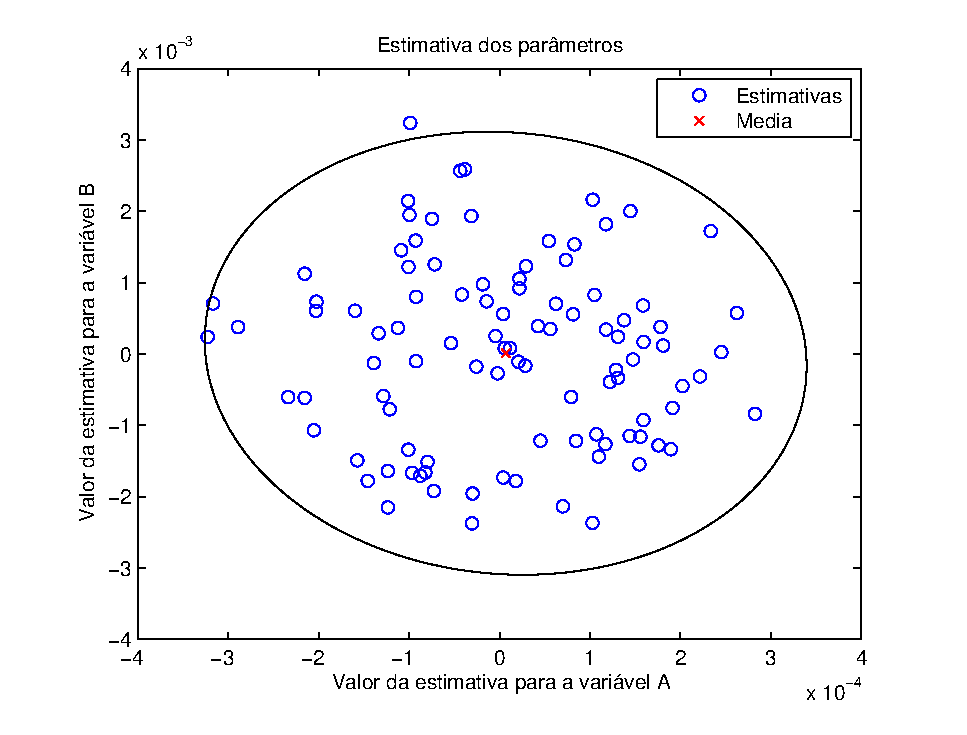
\includegraphics[width=0.8\columnwidth]{figures/si_covar_elipse.eps}
	\caption{Estimativas de um sistema e a elipse representando a regi�o de confian�a para um $\chi$ de 99\%. No centro da
	elipse destaca-se a m�dia de todas as estimativas.}
	\label{fig:si_covar_elipse}
\end{figure}



%===============================================================================
\section{Projeto de Experimento}
\label{sec:si_project_experiments}
%===============================================================================

Projeto de experimentos pode ser entendido como o procedimento para que se escolha o melhor 
sinal de entrada para a identifica��o dos par�metros desejados para o experimento. 
Desta forma muitas vari�veis podem ser levadas em considera��o, refletindo em propriedades que
podem ou n�o ser o foco do projeto de experimentos.

Uma forma de organizar o projeto de experimentos � desenvolv�-lo como um problema de otimiza��o 
convexa, onde entre muitas vantagens est� o fato de que � poss�vel a utiliza��o de m�todos matem�ticos
para o c�lculo e sua formula��o pode ser feita por LMIs ({\it{Linear Matrix Inequality}}). Em \cite{jansson}
este t�pico � explorado em mais profundidade, sendo aqui apenas apresentada a sua ideia b�sica.

A escolha de um sinal mais apropriado para o experimento traz diversas vantagens, que podem ser bastante
significativas para o tempo e esfor�o despendido sobre o projeto do controlador, ou da identifica��o do sistema.
Uma destas vantagens � o tempo de dados coletados; aplicando-se sinais com componentes de frequ�ncia que s�o
mais informativos, tem-se uma efici�ncia maior nos dados amostrados, bastando um montante menor de dados, para que
sejam obtidos os mesmos �ndices de qualidade.

%===============================================================================
\subsection{Sinais de entrada mais comumente utilizados}
\label{sec:si_project_signal_input}
%===============================================================================

V�rios sinais que podem ser gerados de maneira f�cil e que possuem um grande n�mero de componentes de frequ�ncia foram
elaborados.

%===============================================================================
\subsubsection{Sinal Bin�rio Pseudo-Rand�mico - PRBS}
\label{sec:si_project_signal_input_prbs}
%===============================================================================
% ref: ljung pages 418

Um {\it{sinal bin�rio pseudo-rand�mico}} � um sinal peri�dico com algumas propriedades
semelhantes � do ru�do branco. Este sinal � gerado pela equa��o:

\begin{equation}
u(t)=rem(A(q)u(t), 2)=rem(a_1 u(t-1)+...+a_n u(t-n), 2)
\label{eq:si_project_signal_prbs}
\end{equation}
onde $rem(x, 2)$ � o resto inteiro da divis�o de $x$ por 2. O sinal $u(t)$ deve ser peri�dico 
de pelo menos $2^n$ valores diferentes. Como uma sequ�ncia de zeros n�o � um sinal v�lido, por ser nulo, 
temos que o m�ximo per�odo � de tamanho $M=2^n -1$. Na verdade o per�odo vai depender da
escolha de $A(q)$. Pode-se entretanto mostrar que para cada $n$ existem escolhas de $A(q)$ que 
proporcionam o tamanho m�ximo. Tais escolhas s�o apresentadas na Tabela \ref{table:si_project_input_prbs} \cite{ljung}.

\begin{table*}[htbp]
\begin{center}
\caption{Polin�mios $A(q)$ que geram o m�ximo per�odo $M$ para sinais PRBS de ordem $n$. $a_k=1$ para os $k$
   	indicados, 0 para os demais. Diversas outras escolhas existem para os mesmos $n$.}
\label{table:si_project_input_prbs}
\begin{tabular}{ccc}
\hline
        Ordem $n$ & $M=2^n-1$ & $a_k$ n�o zeros para $k$   \\
\hline
        2       & 3        & 1, 2       \\
        3       & 7        & 2, 3       \\
        4       & 15       & 1, 4       \\
        5       & 31       & 2, 5       \\
        6       & 63       & 1, 6       \\
        7       & 127      & 3, 7       \\
        8       & 255      & 1, 2, 7, 8 \\
        9       & 511      & 4, 9       \\
        10      & 1023     & 7, 10      \\
        11      & 2047     & 9, 11      \\
\hline
\end{tabular}
\end{center}
\end{table*}

O espectro de um sinal PRBS � dado por:

\begin{equation}
\Phi_u(\omega)=\frac{2 \pi \bar{u}^2}{M}\sum_{k=1}^{M-1}\delta (\omega -2 \pi k/M), \;\; 0\le \omega < 2 \pi
\label{eq:si_project_signal_prbs_spectrum}
\end{equation}

Observa-se que este � um sinal persistentemente excitante de ordem $M-1$. Na Figura 
\ref{fig:si_project_prbs} � apresentado um exemplo de sinal PRBS para $n=7$.

\begin{figure}[htbp]
	\center
	\includegraphics[width=0.95\columnwidth]{figures/si_project_prbs.eps}
	\caption{Sinal PRBS para $n=7$}
	\label{fig:si_project_prbs}
\end{figure}

%===============================================================================
\subsubsection{Ruido Branco Filtrado}
\label{sec:si_project_signal_input_wn_filtered}
%===============================================================================

Um das escolhas mais simples de sinais, � gerar um ru�do Gausiano e ent�o filtr�-lo com 
algum filtro linear. Desta forma, teoricamente, � poss�vel atingir qualquer espectro de
sinal, bastando apenas a correta escolha do filtro. Como este sinal � gerado {\it{off-line}}, 
� poss�vel aplicar filtros n�o causais e eliminar efeitos transientes do sinal, o que
proporciona um comportamento espectral melhor \cite{campestrini, ljung}.

%===============================================================================
\subsection{Projeto de experimento}
\label{sec:si_project_optimization}
%===============================================================================

O problema de projeto de experimento pode ser considerado como uma forma geral apresentada em:

\begin{equation}
\begin{matrix}
\underset{\Phi_{\chi_0}}{\text{minimize}} &  & \text{Objetivo}\\ 
\text{Sujeito a:} &  & \text{Requisitos de qualidade}\\ 
 &  & \text{Requisitos de sinais}
\end{matrix}
\label{eq:si_project_optimization}
\end{equation}

De forma geral os requisitos de qualidades s�o fun��es da covari�ncia de $P$. Por esta raz�o � natural usar
o espectro da entrada $\Phi_u$ e eventualmente o espectro cruzado $\Phi_{ue}$ como vari�veis do projeto.
A inclus�o de limita��es nos sinais e sua inclus�o como vari�veis de projeto s�o �teis para evitar que se chegue
em resultados onde a energia de entrada precise ser infinita para se obter os crit�rios desejados, ou largura
de banda que n�o s�o facilmente ating�veis em projetos reais.

T�picos projetos de experimentos s�o intrat�veis em sua forma original, pelos seguintes motivos \cite{jansson}: 

\begin{enumerate}[I]
\item Algumas restri��es s�o tipicamente n�o convexas.
\item Existem restri��es que s�o de dimens�o infinita.
\item Existe ainda o problema de encontrar um sinal realiz�vel que tenha as propriedades desejadas para o espectro.
\item A vari�ncia assint�tica depende tipicamente dos par�metros do sistema $\theta_0$, $P=P(\theta_0)$ que s�o
desconhecidos.
\end{enumerate}

Os primeiros 3 itens listados acima s�o contorn�veis pela inser��o de uma parametriza��o finita do espectro de entrada
e algumas vezes at� do espectro cruzado, tornando o problema convexo, que pode ser tratado de forma bem mais f�cil.

O �ltimo item onde a solu��o do problema depende das caracter�sticas do sistema a ser identificado � intr�nseco de quase
todos os problemas de otimiza��o, sendo ent�o inevit�vel. Em problemas reais este fato pode ser contornado utilizando alguns
m�todos conhecidos \cite{jansson}.

A formula��o de um projeto de experimento pode ser particionado nas seguintes partes:

\renewcommand{\labelitemi}{$\bullet$}
\begin{itemize}

\item {\it{Parametriza��o do espectro}}

A escolha de usar uma parametriza��o finita do espectro ou uma parametriza��o parcial da correla��o � regido pelos seguintes
aspectos:

\begin{itemize}
\item Relativos a otimiza��o
\item Computacionais
\item Limita��o de sinais
\item Robustez
\end{itemize}

A parametriza��o parcial da correla��o � �tima e pode usar um n�mero m�nimo de par�metros, utilizando assim, menos processamento
computacional. Entretanto certas limita��es de sinais n�o podem ser garantidas nesta situa��o, e a parametriza��o
pode depender do sistema real. Parametriza��o finita do espectro geralmente n�o atinge um m�nimo global mas as fun��es bases
n�o precisam ser fun��es do sistema real. Este m�todo pode gerenciar problemas de limita��es de sinal de frequ�ncia por frequ�ncia.
%-------------------------
\item {\it{Restri��es de qualidade}}

Assumindo que erros de vari�ncia s�o de grande import�ncia � natural que qualquer medida de qualidade do modelo leve em conta 
a matriz de covari�ncia $P$. Esta matriz pode ser manipulada pelos espectros de entrada $\Phi_{u}$ e o espectro cruzado $\Phi_{ue}$
como apresentado em \eqref{eq:si_project_optimization_quality}.

\begin{equation}
P^{-1}(\theta_0)=\frac{1}{2 \pi \lambda_0}\int_{-\pi}^{\pi}\mathcal{F}(e^{j\omega}, \theta_0)\begin{bmatrix}
\Phi_u(\omega) & \Phi_{ue}(\omega)\\ 
\Phi_{ue}^{0}(\omega) & \lambda_0 
\end{bmatrix}\mathcal{F}(e^{j\omega}, \theta_0)\;d\omega
\label{eq:si_project_optimization_quality}
\end{equation}

O principal desafio neste ponto � tornar as restri��es convexas em $P^{-1}$.

%-------------------------
\item {\it{Restri��es de sinal}}

Podem ser inclu�dos, restri��es de energia para os sinais de entrada e sa�da do sistema bem como restri��es no sinal dependentes da
frequ�ncia deste.
%-------------------------
\item {\it{Restri��es de robustez}}

A solu��o de boa parte dos problemas de otimiza��o recaem na necessidade de se conhecer o sistema real. Isso nem sempre � poss�vel 
e uma das formas de contornar este problema � substituir o sistema real por uma aproxima��o deste. Devido aos erros de estimativa deste
sistema, tem-se a necessidade de se utilizar m�todos que garantam robustez deste sistema, para que quando submetido ao sistema real, 
o projeto ainda seja v�lido.
%-------------------------
\end{itemize}



%===============================================================================
\section{Considera��es Finais}
\label{sec:si_conclusions}
%===============================================================================

Neste cap�tulo foram introduzidos os principais conceitos para a identifica��o de sistemas LTI de tempo discreto. 
A identifica��o de sistemas cont�m tr�s elementos fundamentais: o sistema real $\mathcal{S}$ e o conjunto de
dados coletados deste sistema $Z^N$, a classe de modelos $\mathcal{M}$ escolhida para representar o sistema real e o crit�rio
que elenca qual � o modelo dentro da classe que melhor descreve o sistema real. 

De posse do conjunto de dados, da classe de modelos, e do crit�rio, apresentou-se o m�todo mais comumente utilizado para
identifica��o: M�todo dos m�nimos quadrados. Foram apresentadas suas caracter�sticas e suas propriedades. Devido �s
incertezas da estimativa dos par�metros quando o regressor est� correlacionado com o ru�do, foram introduzidos m�todos
alternativos a este para sanar este problema. Foram apresentados para isso os m�todos das vari�veis instrumentais e
tamb�m o m�todo PEM onde leva-se em conta a modelagem do ru�do na identifica��o.

Apresentou-se as propriedades estat�sticas das estimativas obtidas e quais s�o os erros esperados para situa��es onde a
classe de modelos $\mathcal{M}$ consegue representar o sistema real $\mathcal{S}$ e quando $\mathcal{S} \notin
\mathcal{M}$. Em adi��o a estas propriedades discutiu-se quais s�o as condi��es que propiciam erro de polariza��o e
quais influenciam no erro de vari�ncia das estimativas. Introduziu-se tamb�m o conceito de n�vel de confian�a baseado
nas caracter�sticas do experimento realizado.

Ao fim foram apresentados os principais aspectos de um projeto de identifica��o de sistemas. Partindo-se da escolha do
sinal de excita��o para o experimento onde pode-se determinar o que � de fundamental import�ncia para a identifica��o e
focar os esfor�os para reduzir ao m�ximo erros nestes aspectos. Apresentou-se neste quesito de projeto de experimento, a
ideia de tornar a escolha do sinal, um problema de otimiza��o, onde as restri��es s�o as margens de qualidade que
deseja-se para as propriedades assint�ticas da estimativa, limita��es de sinais e margens de robustez.

� percept�vel que a identifica��o de um sistema � uma tarefa que depende de um conjunto relativamente grande
de fatores. De um lado isso � extremamente interessante, pois tem-se liberdade de escolha e a possibilidade de focar
o projeto em pontos que s�o mais interessantes e importante, em detrimento de outros que n�o s�o relevantes para o
sistema em quest�o. Por outro lado o conjunto de vari�veis que, se n�o compreendidas corretamente, podem tornar este
processo oneroso e por vezes at� ineficiente.


%===============================================================================



%===============================================================================
\chapter{Identifica��o de sistemas n�o lineares de tempo discreto}
\label{chapter:nlin_si_ident}
%===============================================================================
% idea: Colocar aqui neste capitulo todas as defini��es genericas sobre 
% n�o linearidades. coisas que na� sao relacionadas com o que eu vou fazer, ou que n�o
% sao conseguencia dela.
%
% lineariza��o: Descrever que muitas aplica�oes de identifica��o de sis nonlineares �
% linearizar ele em torno de um ponto. que isso ja eh bom suficiente.
%
% Models: Descrever os tipos de modelos para descrever sistemas nao lineares. Aqui 
% da para escrever bastante coisa. existem muito tipo de modelos para isso.
%
% Algoritmos: aqui vai o algoritmo do aguirre para modelos racionais. Talvez fosse de
% pensar em colcar isso no capitulo com minhas contribui��es? acho que nao .. referencio isso
% no meu capitulo.
%
% Conclus�es: Resumo do que foi visto aqui 

Anteriormente foram introduzidos conceitos b�sicos de identifica��o de sistemas lineares invariantes no tempo.
Este capitulo tem como objetivo apresentar os principais conceitos para identifica��o de sistemas n�o lineares de tempo
discreto.

A maioria dos sistemas de controle encontrados na pratica s�o n�o lineares e mesmo podendo ser
caracterizados por um sistema linear quando operando em uma regi�o restrita, a maioria dos sistemas
n�o lineares s� pode ser amplamente caracterizado por um modelo n�o linear.
\cite{billings_nl_survey} 

Na se��o \ref{sec:nlin_si_basic} ser�o apresentados conceitos b�sicos
sobre n�o linearidades. Algumas caracter�sticas de sistemas n�o lineares quando s�o linearizados em
torno de um ponto de opera��o ser�o apresentados na se��o \ref{sec:nlin_si_basic_types}.

Na se��o \ref{sec:nl_models} ser�o apresentados alguns modelos usualmente utilizados para
caracteriza��o de sistemas n�o lineares. Dando enfase aos modelos {\it{NARMAX}} onde na se��o
\ref{sec:nl_si_algorithms_rationals} ser�o apresentados algoritmos utilizados para a identifica��o de
sistemas n�o lineares para este modelo.

Ao fim, ser�o apresentados breves conclus�es sobre identifica��o de sistemas n�o lineares (se��o
\ref{sec:nl_conclusions}).
%===============================================================================
%===============================================================================
\section{Conceitos b�sicos}
\label{sec:nlin_si_basic}
%===============================================================================

Muitos, se n�o todos, os sistemas reais s�o n�o lineares. Existe entretanto um grande n�mero destes sistemas que
podem, e assim o s�o, representados por sistemas lineares em determinadas faixas de opera��o. Os sistemas desta
forma conseguem representar satisfat�riamente o sistema observado. Todavia alguns sistemas para serem
linearizados exigem uma faixa de atua��o muito estreita, fazendo com que o sistema em sua opera��o normal j� saida desta faixa,
tornando o modelo linear n�o representativo para aquele sistema em quest�o.

Tem-se desta forma uma das justificativas de escolher um modelo n�o linear para caracterizar o sistema. Ganha-se de um
lado no quesito de faixa de atua��o mais ampla e perde-se por abdicar da simplicidade de sistemas lineares.

Um sistema n�o linear pode ser genericamente descrito por:

\begin{equation}
y(t)=f(u(t), e(t))
\label{eq:nlin_system}
\end{equation}

onde $f(\cdot)$ � uma fun��o n�o linear dependente do sinal de entrada $u(t)$, e do ru�do do sistema $e(t)$. $y(t)$
� definido como a sa�da deste sistema.

%===============================================================================
\subsection{Tipos de n�o linearidades}
\label{sec:nlin_si_basic_types}
%===============================================================================
% Khalil
% ljng 		142
% Aguirre

Existem duas limita��es b�sicas para sistemas linearizados. Primeiro que a lineariza��o
� uma aproxima��o ao redor do ponto de opera��o, logo ele pode prever apenas o comportamento
nesta localidade do sistema e n�o o comportamento global. Segundo, as din�micas
de sistemas n�o lineares s�o muito mais ricas que as de sistemas lineares. Existem portanto alguns
fen�menos {\it{essenciais}}, n�o lineares, que n�o conseguem ser descritos ou
preditos por modelos lineares, estes s�o: \cite{khalil}

\renewcommand{\labelitemi}{$\bullet$}
\begin{itemize}

\item Tempo de fuga finito

O estado de um sistema linear inst�vel tende ao infinito na medida que o tempo 
tende ao infinito. Um sistema n�o linear est�vel, entretanto, pode ir para o
infinito em um tempo finito.


\item M�ltiplos pontos de equil�brios isolados

Um sistema linear assint�ticamente est�vel tem apenas um ponto de equil�brio. Desta forma, este sistema pode
ter apenas um ponto do espa�o de estados que atraem o estado do sistema, independentemente
do estado inicial. Um sistema n�o linear pode ter mais de um ponto de equil�brio isolado. 
Desta forma o estado do sistema pode convergir para um destes equil�brios ou outro,
dependendo do estado inicial do sistema.

\item Ciclos limites

Para um sistema linear e invariante no tempo oscilar ele deve ter um par de autovalores
sobre o eixo imagin�rio, o que � uma condi��o n�o robusta praticamente imposs�vel de manter
na presen�a de perturba��es. Mesmo que isso seja poss�vel de manter, a amplitude da 
oscila��o depender� das condi��es iniciais do sistema. Na vida real, oscila��es est�veis
s�o atingidas apenas com sistemas n�o lineares. Alguns sistemas possuem oscila��es com
amplitude e frequ�ncia constantes, independente das condi��es iniciais. Chama-se isso de
ciclos limites.

\item Sub harm�nicas, harm�nicas ou oscila��es quase peri�dicas 

Um sistema linear est�vel sob uma entrada senoidal peri�dica produz uma sa�da senoidal na mesma frequ�ncia.
Sistemas n�o lineares alimentados por sinais peri�dicos podem oscilar com frequ�ncias que
podem ser sub m�ltiplos ou m�ltiplos da frequ�ncia de entrada.

\item Caos

Um sistema n�o linear pode ter um espa�o de estados mais complexo e seu comportamento n�o 
pode ser descrito por equilibrio, oscila��es peri�dicas ou quase peri�dicas. Este comportamento
normalmente � conhecido como caos. Alguns destes movimentos ca�ticos exibem comportamento
rand�mico, independentemente da natureza do sistema.

\item M�ltiplos modos de comportamento

N�o � incomum para dois ou mais modelos exibirem o comportamentos diferentes para um mesmo sistema n�o-linear.Um sistema
n�o for�ado pode ter mais de um ciclo limite. Um sistema for�ado com excita��o pode exibir hamonicas, subharmonicas, ou
comportamentos mais complicados, dependendo da frequ�ncia e amplitude da entrada. Ele pode exibir um pulo descontinuo no
modo de comportmento mesmo com mudan�as pequenas na amplitude e frequ�ncia de entrada do sinal.

\end{itemize}




%===============================================================================
\section{Modelos para sistemas n�o lineares}
\label{sec:nl_models}
%===============================================================================
% ideia aqui � colocar uma pequena introdu��o sobre modelos.. no mesmo estilo
% que foi para sistemas lineares.

Fam�lias ou conjuntos de modelos para sistemas podem ser divididos em dois grupos principais, baseados na natureza de
suas n�o linearidades: n�o linearidades est�ticas, onde a din�mica do sistema pode ser bem caracterizada por um modelo
linear enquanto que a parte n�o linear est� concentrada ou na entrada ou na sa�da do sistema de forma est�tica.
Estes sistemas s�o chamadosde Wiener para n�o linearidades na sa�da do processo ou Hammerstein, quando a
n�o linearidade est� na entrada do processo.

Para os demais casos, onde a n�o linearidade est� na din�mica do processo existem v�rias fam�lias de modelos
que podem ser utilizados como ser� visto no decorrer deste cap�tulo. De forma geral todos estes conjuntos
possuem em comum a ideia da escolha de uma base que seja representativa e que possa reduzir a quantidade de
termos a ser identificado e com isso ter uma boa aproxima��o do sistema real com a menor quantidade de
par�metros poss�vel na identifica��o.

Percebe-se ent�o que um mesmo sistema pode ser representado por diversos destes modelos, mas dependendo das
caracter�sticas deste sistema, uma das fam�lias ser� mais adequada, por sua base possuir mais
afinidade em representar certos tipos de n�o linearidades.

Um dos passos mais desafiadores na constru��o de modelos n�o lineares � a escolha da estrutura de
modelo. Quando este modelo � n�o linear, existe uma grande quantidade de op��es e com isso o perigo
de escolher um modelo desnecessariamente complexo � evidente. este perigo baseia-se no {\it{principio
da parcim�nia}} que basicamente determina que o modelo deve ser o mais simples poss�vel.
\cite{aguirre_maps}

%TODO: achar onde por isso e se nao tem nada melhor no paper para adicionar
%Um problema fundamental referente a modelos parametrizados refere-se ao fato do
%par�metro poder ou n�o ser determinado a partir dos valores medidos de entrada e sa�da. \cite{glad_ljung}

% ===============================================================================
\subsection{Modelos de Wiener e Hammerstein}
\label{sec:nl_models_wiener_hammerstein}
% Aguirre: 334
% ljung 143
%===============================================================================

Modelos de Wiener e Hammerstein s�o normalmente utilizados em situa��es onde a din�mica do sistema pode ser bem
descrita por um sistema linear, mas existem algumas n�o linearidades est�ticas atreladas � entrada
e/ou � sa�da. Este ser� o caso de atuadores n�o lineares com caracter�sticas como satura��o, zona morta, entre outros.

Um modelo com n�o linearidades na entrada � chamado de {\it{modelo de Hammerstein}} e 
para n�o linearidades na sa�da chama-se {\it{modelo de Wiener}}. \cite{ljung}

Na Figura (\ref{fig:nl_models_hammerstein_wiener}) observa-se o diagrama de bloco para os modelos
de Hammerstein e Wiener.


\begin{figure}[htbp]
\center
\scalebox{1} % Change this value to rescale the drawing.
{
\begin{pspicture}(0,-1.6)(9.439062,1.6)
\usefont{T1}{ptm}{m}{n}
\rput(0.52453125,1.31){$u(t)$}
\usefont{T1}{ptm}{m}{n}
\rput(3.9557812,1.31){$f(u(t))$}
\usefont{T1}{ptm}{m}{n}
\rput(7.554531,1.35){$y(t)$}
\usefont{T1}{ptm}{m}{n}
\rput(5.8759375,1.15){Modelo}
\usefont{T1}{ptm}{m}{n}
\rput(5.7834377,0.75){Linear}
\usefont{T1}{ptm}{m}{n}
\rput(2.1957812,1.03){$f(\cdot)$}
\psframe[linewidth=0.04,dimen=outer](3.0,1.6)(1.2,0.4)
\psframe[linewidth=0.04,dimen=outer](6.8,1.6)(5.0,0.4)
\psline[linewidth=0.04cm,arrowsize=0.05291667cm 2.0,arrowlength=1.4,arrowinset=0.4]{->}(3.0,1.0)(5.0,1.0)
\psline[linewidth=0.04cm,arrowsize=0.05291667cm 2.0,arrowlength=1.4,arrowinset=0.4]{->}(0.0,1.0)(1.2,1.0)
\psline[linewidth=0.04cm,arrowsize=0.05291667cm 2.0,arrowlength=1.4,arrowinset=0.4]{->}(6.8,1.0)(8.0,1.0)
\usefont{T1}{ptm}{m}{n}
\rput(0.52453125,-0.69){$u(t)$}
\usefont{T1}{ptm}{m}{n}
\rput(3.9357812,-0.69){$z(t)$}
\usefont{T1}{ptm}{m}{n}
\rput(2.0759375,-0.85){Modelo}
\usefont{T1}{ptm}{m}{n}
\rput(1.9834375,-1.25){Linear}
\usefont{T1}{ptm}{m}{n}
\rput(5.9957814,-0.99){$f(\cdot)$}
\psframe[linewidth=0.04,dimen=outer](3.0,-0.4)(1.2,-1.6)
\psframe[linewidth=0.04,dimen=outer](6.8,-0.4)(5.0,-1.6)
\psline[linewidth=0.04cm,arrowsize=0.05291667cm 2.0,arrowlength=1.4,arrowinset=0.4]{->}(3.0,-1.0)(5.0,-1.0)
\psline[linewidth=0.04cm,arrowsize=0.05291667cm 2.0,arrowlength=1.4,arrowinset=0.4]{->}(0.0,-1.0)(1.2,-1.0)
\psline[linewidth=0.04cm,arrowsize=0.05291667cm 2.0,arrowlength=1.4,arrowinset=0.4]{->}(6.8,-1.0)(8.0,-1.0)
\usefont{T1}{ptm}{m}{n}
\rput(8.204532,-0.65){$y(t)=f(z(t))$}
\end{pspicture} 
}
\caption{Acima: modelo de Hammerstein. Abaixo: Modelo de Wiener.}
\label{fig:nl_models_hammerstein_wiener}
\end{figure}

%===============================================================================
\subsection{Serie de volterra}
\label{sec:nl_models_volterra}
% Aguirre 334
%===============================================================================

Um sistema n�o linear pode ser descrito pela s�rie de Volterra \eqref{eq:nl_models_volterra}:

\begin{equation}
y(t)=\sum_{j=1}^{\infty}\int_{-\infty}^{\infty}\cdots \int_{-\infty}^{\infty}
h_j(\tau_1, ... ,\tau_j) \prod_{i=1}^{j}u(t-\tau_i)d\tau_i
\label{eq:nl_models_volterra}
\end{equation}

onde $h_j$ s�o generaliza��es n�o lineares da resposta ao impulso $h_1(t)$ . Para
um sistema linear com $j=1$ a equa��o de Volterra se reduz � integral de convolu��o.
\cite{aguirre}

As expans�es funcionais em s�ries de Volterra relacionam os sinais passados da entrada com o valor atual da sa�da do
sistema e isso inevitavelmente significa que que um conjunto relativamete elevado de par�metros � necess�rio para
descrever at� mesmo simples sistemas n�o lineares e consequentemente apenas poucas aplica��es pr�ticas foram apresentadas.
\cite{chen_billings1989}

%===============================================================================
\subsection{Redes Neurais}
\label{sec:nl_models_neurals}
% TODO: Search for bib
%===============================================================================
As redes neurais artificiais s�o compostas por camadas de neur�nios interconectados. A sa�da de um
neur�nio com $n$ entradas � apresentada na equa��o \eqref{eq:nl_models_neural}

\begin{equation}
x=\emph{f}\left ( \sum_{j=1}^{n}\omega_j x_j +b \right )
\label{eq:nl_models_neural}
\end{equation}

Sendo $b$ (bias) e $\omega_j$ constantes e $\emph{f}(\cdot)$ � chamada fun��o de ativa��o. A
fun��o de ativa��o mais comum �: \cite{aguirre}

\begin{equation}
\emph{f}(z)=\frac{1}{1+e^{-z}}
\nonumber
\end{equation}


%===============================================================================
\subsubsection{Redes Neurais multi-camadas}
\label{sec:nl_models_neurals_multilayer}
%===============================================================================

Uma t�pica rede multi-camadas pode ser descrita como na Figura
(\ref{fig:nl_models_neural_multilayer}).  Na pr�tica redes neurais multi-camadas t�m grande apelo no
reconhecimento de padr�es. Do ponto de vista te�rico os sistemas de redes multi-camadas podem ser
considerados como mapas n�o lineares onde os elementos das matrizes de peso s�o os par�metros.
\cite{narenda_parthasarathy}

\begin{figure}[htbp]
\center
\scalebox{0.85} % Change this value to rescale the drawing.
{
\begin{pspicture}(0,-3.369375)(14.589063,3.329375)
\pscircle[linewidth=0.04,dimen=outer](4.77,2.729375){0.4}
\usefont{T1}{ptm}{m}{n}
\rput(4.804531,2.699375){$\sum$}
\psframe[linewidth=0.04,dimen=outer](7.17,3.329375)(5.97,2.129375)
\usefont{T1}{ptm}{m}{n}
\rput(6.534531,2.759375){$\gamma$}
\pscircle[linewidth=0.04,dimen=outer](4.77,0.529375){0.4}
\usefont{T1}{ptm}{m}{n}
\rput(4.804531,0.499375){$\sum$}
\psframe[linewidth=0.04,dimen=outer](7.17,1.129375)(5.97,-0.070625)
\usefont{T1}{ptm}{m}{n}
\rput(6.534531,0.559375){$\gamma$}
\pscircle[linewidth=0.04,dimen=outer](4.77,-1.870625){0.4}
\usefont{T1}{ptm}{m}{n}
\rput(4.804531,-1.900625){$\sum$}
\psframe[linewidth=0.04,dimen=outer](7.17,-1.270625)(5.97,-2.470625)
\usefont{T1}{ptm}{m}{n}
\rput(6.534531,-1.840625){$\gamma$}
\pscircle[linewidth=0.04,dimen=outer](10.37,2.729375){0.4}
\usefont{T1}{ptm}{m}{n}
\rput(10.384531,2.679375){$\sum$}
\psframe[linewidth=0.04,dimen=outer](12.77,3.329375)(11.57,2.129375)
\usefont{T1}{ptm}{m}{n}
\rput(12.254531,2.739375){$\gamma$}
\pscircle[linewidth=0.04,dimen=outer](10.37,0.529375){0.4}
\usefont{T1}{ptm}{m}{n}
\rput(10.384531,0.479375){$\sum$}
\psframe[linewidth=0.04,dimen=outer](12.77,1.129375)(11.57,-0.070625)
\usefont{T1}{ptm}{m}{n}
\rput(12.254531,0.539375){$\gamma$}
\pscircle[linewidth=0.04,dimen=outer](10.37,-1.870625){0.4}
\usefont{T1}{ptm}{m}{n}
\rput(10.384531,-1.920625){$\sum$}
\psframe[linewidth=0.04,dimen=outer](12.77,-1.270625)(11.57,-2.470625)
\usefont{T1}{ptm}{m}{n}
\rput(12.254531,-1.860625){$\gamma$}
\psline[linewidth=0.04cm,arrowsize=0.05291667cm 2.0,arrowlength=1.4,arrowinset=0.4]{->}(5.17,2.729375)(5.97,2.729375)
\psline[linewidth=0.04cm,arrowsize=0.05291667cm 2.0,arrowlength=1.4,arrowinset=0.4]{->}(5.17,0.529375)(5.97,0.529375)
\psline[linewidth=0.04cm,arrowsize=0.05291667cm 2.0,arrowlength=1.4,arrowinset=0.4]{->}(5.37,-1.870625)(5.97,-1.870625)
\psline[linewidth=0.04cm,arrowsize=0.05291667cm 2.0,arrowlength=1.4,arrowinset=0.4]{->}(10.77,2.729375)(11.57,2.729375)
\psline[linewidth=0.04cm,arrowsize=0.05291667cm 2.0,arrowlength=1.4,arrowinset=0.4]{->}(10.77,0.529375)(11.57,0.529375)
\psline[linewidth=0.04cm,arrowsize=0.05291667cm 2.0,arrowlength=1.4,arrowinset=0.4]{->}(10.77,-1.870625)(11.57,-1.870625)
\psline[linewidth=0.04cm,arrowsize=0.05291667cm 2.0,arrowlength=1.4,arrowinset=0.4]{->}(12.77,2.729375)(13.97,2.729375)
\psline[linewidth=0.04cm,arrowsize=0.05291667cm 2.0,arrowlength=1.4,arrowinset=0.4]{->}(12.77,0.529375)(13.97,0.529375)
\psline[linewidth=0.04cm,arrowsize=0.05291667cm 2.0,arrowlength=1.4,arrowinset=0.4]{->}(12.77,-1.870625)(13.97,-1.870625)
\usefont{T1}{ptm}{m}{n}
\rput(13.674531,3.039375){$y_1$}
\usefont{T1}{ptm}{m}{n}
\rput(13.674531,0.839375){$y_2$}
\usefont{T1}{ptm}{m}{n}
\rput(13.674531,-1.560625){$y_n$}
\psdots[dotsize=0.12](6.77,-0.470625)
\psdots[dotsize=0.12](6.77,-0.670625)
\psdots[dotsize=0.12](6.77,-0.870625)
\psdots[dotsize=0.12](12.37,-0.470625)
\psdots[dotsize=0.12](12.37,-0.670625)
\psdots[dotsize=0.12](12.37,-0.870625)
\psline[linewidth=0.04cm,arrowsize=0.05291667cm 2.0,arrowlength=1.4,arrowinset=0.4]{->}(7.1873198,2.729375)(9.97,2.729375)
\psline[linewidth=0.04cm,arrowsize=0.05291667cm 2.0,arrowlength=1.4,arrowinset=0.4]{->}(7.1873198,2.729375)(9.97,0.529375)
\psline[linewidth=0.04cm,arrowsize=0.05291667cm 2.0,arrowlength=1.4,arrowinset=0.4]{->}(7.1873198,2.729375)(9.97,-1.870625)
\psline[linewidth=0.04cm,arrowsize=0.05291667cm 2.0,arrowlength=1.4,arrowinset=0.4]{->}(7.1873198,0.529375)(9.97,0.529375)
\psline[linewidth=0.04cm,arrowsize=0.05291667cm 2.0,arrowlength=1.4,arrowinset=0.4]{->}(7.1873198,-1.870625)(9.97,-1.870625)
\psline[linewidth=0.04cm,arrowsize=0.05291667cm 2.0,arrowlength=1.4,arrowinset=0.4]{->}(7.1873198,0.529375)(9.97,2.729375)
\psline[linewidth=0.04cm,arrowsize=0.05291667cm 2.0,arrowlength=1.4,arrowinset=0.4]{->}(7.1873198,0.529375)(9.97,-1.870625)
\psline[linewidth=0.04cm,arrowsize=0.05291667cm 2.0,arrowlength=1.4,arrowinset=0.4]{->}(7.1873198,-1.870625)(9.97,0.529375)
\psline[linewidth=0.04cm,arrowsize=0.05291667cm 2.0,arrowlength=1.4,arrowinset=0.4]{->}(7.1873198,-1.870625)(9.97,2.729375)
\psline[linewidth=0.04cm,arrowsize=0.05291667cm 2.0,arrowlength=1.4,arrowinset=0.4]{->}(1.7888126,2.7075653)(4.37,2.7075653)
\psline[linewidth=0.04cm,arrowsize=0.05291667cm 2.0,arrowlength=1.4,arrowinset=0.4]{->}(1.7888126,2.7075653)(4.37,0.51799595)
\psline[linewidth=0.04cm,arrowsize=0.05291667cm 2.0,arrowlength=1.4,arrowinset=0.4]{->}(1.7888126,2.7075653)(4.37,-1.870625)
\psline[linewidth=0.04cm,arrowsize=0.05291667cm 2.0,arrowlength=1.4,arrowinset=0.4]{->}(1.7871279,0.529375)(4.37,0.529375)
\psline[linewidth=0.04cm,arrowsize=0.05291667cm 2.0,arrowlength=1.4,arrowinset=0.4]{->}(1.7871279,-1.850625)(4.37,-1.850625)
\psline[linewidth=0.04cm,arrowsize=0.05291667cm 2.0,arrowlength=1.4,arrowinset=0.4]{->}(1.7871279,0.529375)(4.37,2.729375)
\psline[linewidth=0.04cm,arrowsize=0.05291667cm 2.0,arrowlength=1.4,arrowinset=0.4]{->}(1.7871279,0.529375)(4.37,-1.870625)
\psline[linewidth=0.04cm,arrowsize=0.05291667cm 2.0,arrowlength=1.4,arrowinset=0.4]{->}(1.7871279,-1.850625)(4.37,0.5389402)
\psline[linewidth=0.04cm,arrowsize=0.05291667cm 2.0,arrowlength=1.4,arrowinset=0.4]{->}(1.7871279,-1.850625)(4.37,2.729375)
\usefont{T1}{ptm}{m}{n}
\rput(1.4745313,3.039375){$u_1$}
\usefont{T1}{ptm}{m}{n}
\rput(1.4745313,0.839375){$u_2$}
\usefont{T1}{ptm}{m}{n}
\rput(1.4745313,-1.560625){$u_n$}
\usefont{T1}{ptm}{m}{n}
\rput(1.4845313,-3.160625){$\text{Entrada}$}
\usefont{T1}{ptm}{m}{n}
\rput(6.7345314,-3.160625){$\text{Camada Oculta}$}
\usefont{T1}{ptm}{m}{n}
\rput(12.444531,-3.160625){$\text{Camada Sa�da}$}
\end{pspicture} 
}

\caption{Rede neural multi-camadas.}
\label{fig:nl_models_neural_multilayer}
\end{figure}

A sa�da do sistema para uma rede multi-camadas pode ser descrita como:

\begin{equation}
y(t)=f_s\left \{ \sum_{i=1}^{m} \omega_i f_i \left ( \sum_{j=1}^{n}\omega_{ij} x_j + b_i \right ) +
b_s \right \}
\label{eq:nl_models_neural_multilayer}
\end{equation}

Sendo que $f_s$ � a fun��o de ativa��o do neur�nio da camada de sa�da. Esta fun��o n�o precisa ser
igual a $f_i$, $i=1, \ldots , m$ que por sua vez n�o precisam ser iguais entre si. As constantes $b_s$ s�o os termos
de polariza��o dos neur�nios da camada de sa�da, $\omega_i$ s�o os pesos da sa�da de cada neur�nio da
camada oculta e $\omega_{ij}$ s�o os pesos da entrada $j$, vista pelo $i-$�simo neur�nio da camada
oculta. \cite{aguirre}

%===============================================================================
\subsubsection{Redes Neurais recorrentes}
\label{sec:nl_models_neurals_multilayer}
%===============================================================================

Redes neurais recorrentes, trabalho introduzido por Hopfield em \cite{hopfield} prov� uma
alternativa para o reconhecimento de padr�es. O m�todo proposto consiste em ter uma rede neural de
apenas uma camada adicionada de uma realimenta��o com um atraso de tempo como apresentado na Figura
(\ref{fig:nl_models_neural_recurrent}). \cite{narenda_parthasarathy}

\begin{figure}[htbp]
\center
\scalebox{0.85} % Change this value to rescale the drawing.
{
\begin{pspicture}(0,-5.4)(11.04,5.4)
\usefont{T1}{ptm}{m}{n}
\rput(8.015624,4.91){$\gamma$}
\usefont{T1}{ptm}{m}{n}
\rput(8.015624,3.31){$\gamma$}
\usefont{T1}{ptm}{m}{n}
\rput(8.215624,0.71){$\gamma$}
\usefont{T1}{ptm}{m}{n}
\rput(5.073437,-0.89){$z^{-1}$}
\pscircle[linewidth=0.04,dimen=outer](6.42,4.8){0.4}
\pscircle[linewidth=0.04,dimen=outer](6.42,0.6){0.4}
\pscircle[linewidth=0.04,dimen=outer](6.42,3.2){0.4}
\usefont{T1}{ptm}{m}{n}
\rput(6.395625,0.61){$\sum$}
\usefont{T1}{ptm}{m}{n}
\rput(6.395625,3.21){$\sum$}
\usefont{T1}{ptm}{m}{n}
\rput(6.395625,4.81){$\sum$}
\psdots[dotsize=0.12](5.82,4.8)
\psdots[dotsize=0.12](5.82,3.2)
\psdots[dotsize=0.12](5.82,0.6)
\psdots[dotsize=0.12](2.82,4.8)
\psdots[dotsize=0.12](2.82,3.2)
\psdots[dotsize=0.12](2.82,0.6)
\psline[linewidth=0.04cm](2.82,4.8)(5.82,4.8)
\psline[linewidth=0.04cm](2.82,4.8)(5.82,3.1916058)
\psline[linewidth=0.04cm](2.82,4.8)(5.82,0.61817497)
\psline[linewidth=0.04cm](2.82,0.61817497)(5.82,4.8)
\psline[linewidth=0.04cm](2.82,3.1916058)(5.82,4.8)
\psline[linewidth=0.04cm](2.82,3.1916058)(5.82,3.1916058)
\psline[linewidth=0.04cm](2.82,3.1916058)(5.82,0.61817497)
\psline[linewidth=0.04cm](2.82,0.61817497)(5.82,3.1916058)
\psline[linewidth=0.04cm](2.82,0.61817497)(5.82,0.61817497)
\psline[linewidth=0.04cm](8.8,0.6)(9.42,0.6)
\psline[linewidth=0.04cm](9.4,-1.0)(5.8,-1.0)
\psline[linewidth=0.04cm](4.62,-1.0)(1.6,-1.0)
\psline[linewidth=0.04cm](1.62,0.6)(2.82,0.6)
\psline[linewidth=0.04cm](6.82,0.6)(7.62,0.6)
\psline[linewidth=0.04cm](5.82,0.6)(6.0,0.6)
\psline[linewidth=0.04cm](6.82,3.2)(7.62,3.2)
\psline[linewidth=0.04cm](5.82,3.2)(6.02,3.2)
\psline[linewidth=0.04cm](5.82,4.8)(6.02,4.8)
\psline[linewidth=0.04cm](6.82,4.8)(7.62,4.8)
\psline[linewidth=0.04cm](8.8,3.2)(10.22,3.2)
\psline[linewidth=0.04cm](5.8,-2.6)(10.2,-2.6)
\psline[linewidth=0.04cm](8.8,4.8)(11.02,4.8)
\psline[linewidth=0.04cm](11.0,-4.8)(5.8,-4.8)
\psline[linewidth=0.04cm](4.62,-2.6)(0.8,-2.6)
\psline[linewidth=0.04cm](0.8,3.2)(2.82,3.2)
\psline[linewidth=0.04cm](2.82,4.8)(0.0,4.8)
\psline[linewidth=0.04cm](0.0,-4.8)(4.62,-4.8)
\psdots[dotsize=0.12](8.22,2.2)
\psdots[dotsize=0.12](8.22,2.0)
\psdots[dotsize=0.12](8.22,1.8)
\psdots[dotsize=0.12](5.22,-3.4)
\psdots[dotsize=0.12](5.22,-3.6)
\psdots[dotsize=0.12](5.22,-3.8)
\usefont{T1}{ptm}{m}{n}
\rput(9.864062,5.11){$x_1(t+1)$}
\usefont{T1}{ptm}{m}{n}
\rput(9.864062,3.51){$x_2(t+1)$}
\usefont{T1}{ptm}{m}{n}
\rput(9.864062,0.91){$x_n(t+1)$}
\usefont{T1}{ptm}{m}{n}
\rput(2.0040624,5.11){$x_1(t)$}
\usefont{T1}{ptm}{m}{n}
\rput(2.0040624,3.51){$x_2(t)$}
\usefont{T1}{ptm}{m}{n}
\rput(2.0040624,0.91){$x_n(t)$}
\usefont{T1}{ptm}{m}{n}
\rput(4.3840623,5.11){$\omega_i$}
\usefont{T1}{ptm}{m}{n}
\rput(5.073437,-2.49){$z^{-1}$}
\usefont{T1}{ptm}{m}{n}
\rput(5.073437,-4.69){$z^{-1}$}
\psframe[linewidth=0.04,dimen=outer](8.8,5.4)(7.6,4.2)
\psframe[linewidth=0.04,dimen=outer](8.8,3.8)(7.6,2.6)
\psframe[linewidth=0.04,dimen=outer](8.8,1.2)(7.6,0.0)
\psframe[linewidth=0.04,dimen=outer](5.8,-0.4)(4.6,-1.6)
\psframe[linewidth=0.04,dimen=outer](5.8,-2.0)(4.6,-3.2)
\psframe[linewidth=0.04,dimen=outer](5.8,-4.2)(4.6,-5.4)
\psline[linewidth=0.04cm](11.0,4.8)(11.0,-4.8)
\psline[linewidth=0.04cm](10.2,3.2)(10.2,-2.6)
\psline[linewidth=0.04cm](9.4,0.6)(9.4,-1.0)
\psline[linewidth=0.04cm](1.6,0.6)(1.6,-1.0)
\psline[linewidth=0.04cm](0.8,-2.6)(0.8,3.2)
\psline[linewidth=0.04cm](0.0,4.8)(0.0,-4.8)
\end{pspicture} 
}
\caption{Rede neural recorrentes.}
\label{fig:nl_models_neural_recurrent}
\end{figure}

%===============================================================================
\subsection{Fun��es Radiais de Base}
\label{sec:nl_models_radiais}
% Aguirre 337
%===============================================================================

Fun��es radiais de base  ({\it{RBF - Radial basis functions}})  s�o uma tradicional t�cnica para
interpola��o em espa�os multidimensional \cite{chen_billings_narmax} e podem ser descritas como
mapeamentos do tipo:

\begin{equation}
f(y)=w_0+\sum_{i}w_i \phi (\left \| y-c_i \right \|)
\label{eq:nl_models_rbf}
\end{equation}

Sendo que $y \in \mathbb{R}^{d_e}$ ($d_e$ � conhecido como dimens�o de imers�o),
$\left \| \cdot \right \|$ � a norma euclidiana, $w_i \in \mathbb{R}$ s�o pesos, 
$c_i \in \mathbb{R}^{d_e}$ s�o centros e $\phi(\cdot):\mathbb{R}^+ \to \mathbb{R}$ 
� uma fun��o, normalmente escolhida a priori, como por exemplo: \cite{aguirre}

\begin{equation}
\phi(\left \| y-c_i \right \|)= exp\left ( -\frac{\left \| y-c_i \right \|^2}{\sigma_i^2} \right )
\nonumber
\end{equation}

Outras fun��es de base usadas s�o apresentadas na Tabela (\ref{table:nl_models_rbf})

\begin{table*}[htbp]
\begin{center}
\caption{Algumas fun��es Radiais de base comumente utilizadas.}
\label{table:nl_models_rbf}
\begin{tabular}{ll}
\hline
        Nome & Fun��o   \\
\hline
        Multi quadr�tica inversa  & $\phi(r)=(r^2+\sigma ^2)^{-1/2}$ \\ 
        Linear                    & $\phi(r)=r$                      \\ 
        C�bica                    & $\phi(r)=r^3$                    \\ 
        Multi-quadr�tica           & $\phi(r)=\sqrt{r^2+\sigma^2}$    \\ 
        {\it{Thin - plate spline}} & $\phi(r)=r^2\; \text{log}(r)$   \\ 
\hline
\end{tabular}
\end{center}
\end{table*}

onde $r=\left \| y-c_i \right \|$ e $\sigma$ definem a largura do chap�u no caso de
fun��es Gausianas e das multi-quadr�ticas, como pode ser visto na figura (\ref{fig:nl_models_rbf}).

\begin{figure}[htbp]
	\center
	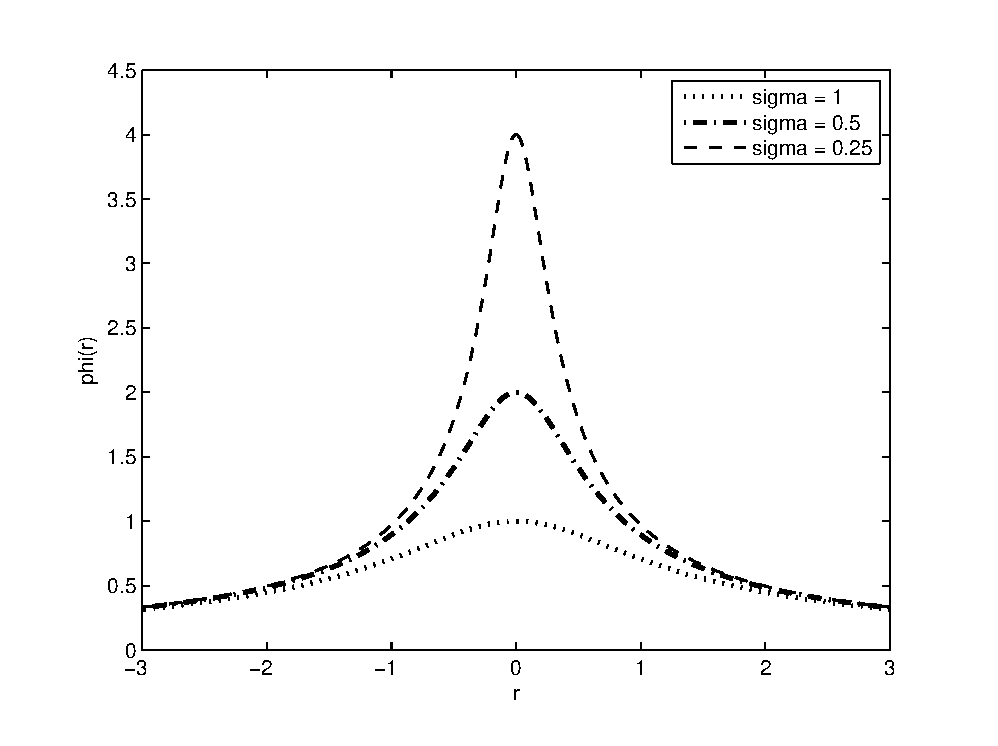
\includegraphics[width=0.8\columnwidth]{figures/nl_models_rbf.eps}
	\caption{Fun��o multiquadr�ticas inversa para alguns valores de $\sigma$.}
	\label{fig:nl_models_rbf}
\end{figure}

Este tipo de representa��o tem boas propriedades locais e pode ser interpretada como 
uma t�cnica de interpola��o global. Fun��es radiais de base s�o casos particulares
de redes neurais, porem neste caso lineares nos par�metros $w_i$.\cite{aguirre} 

No contexto de identifica��o de sistemas � comum adicionar termos auto-regressivos
lineares, bem como termos de entrada � equa��o \eqref{eq:nl_models_rbf} resultando em:

\begin{equation}
y(k)=w_0 + \sum_{i}w_i \phi(\left \| \mathbf{y}(k-1)-c_i \right \|)+\sum_{i=1}^{n_y}a_i y(k-i)+\sum_{i=1}^{n_u}b_i u(k-i)+e(k)
\nonumber
\end{equation}

Sendo $\mathbf{y}(k-1)=\begin{bmatrix}
y(k-1) & ... & y(k-n_y) & u(k-1) & ... & u(k-n_u)
\end{bmatrix}$.

%===============================================================================
\section{Modelos NARMAX}
\label{sec:nl_models_narmax}
% Aguirre 343
%===============================================================================

Os modelos {\it{NARX}} (do termo ingles {\it{nonlinear autoregressive model with
exogenous variables}}) s�o modelos discretos no tempo que caracterizam o valor da sa�da em fun��o
dos valor passados da entrada e da pr�pria sa�da. Algumas vezes, para evitar a polariza��o da estimativa dos
par�metros adiciona-se termos do modelo do ruido ao modelo do sistema. Quando isso � feito o modelo passa a ser chamado
de modelo {\it{NARMAX}} (do termo ingl�s {\it{nonlinear autoregressive moving average model with
exogenous variables}}), introduzido por \cite{leontaritis_billings1985}.

Este modelo prov� uma representa��o unificada para a descri��o de sistemas discretos n�o lineares
\cite{chen_billings_narmax}

Leontaritis e Billings rigorosamente provaram que um sistema n�o linear de tempo discreto (LTI) pode sempre ser
representado por um modelo do tipo \cite{chen_billings1989}:

\begin{equation}
y(t)=F(y(t-1), \cdots, y(t-n_y),u(t-1), \cdots, u(t-n_u) )
\label{eq:nlin_models_narmax_generic}
\end{equation}

Em uma regi�o ao redor do ponto de equil�brio sujeito a duas condi��es:

\begin{enumerate}
\item a resposta da fun��o $F(\cdot)$ do sistema deve ser finitamente realiz�vel.
\item Um modelo linearizado existe se o sistema � operado pr�ximo ao ponto de equil�brio escolhido.
\end{enumerate}

Observa-se que a condi��o (1) apenas exclui sistemas de par�metros distribu�dos e a condi��o (2) implica que se o
sistema for perturbado com uma amplitude pequena, em volta da regi�o do ponto de equil�brio, um modelo linearizado do
sistema existe. \cite{chen_billings1989}

O modelo {\it{NARMAX}} surgiu, ou foi motivado, pelo excessivo esfor�o para a estimativa dos
par�metros e pela dificuldade em interpretar os resultados obtidos com modelos baseados em series
(Wienner, Hammerstein e Volterra). A necessidade do uso de entradas espaciais s�o tamb�m uma
desvantagem destes modelos. \cite{leontaritis_billings1985}

\begin{eqnarray}\nonumber
y(t)&=&F [ y(t-1), ..., y(t-n_y), u(t-1), ... , u(t-n_u),\\
&&  e(t),e(t-1), ... , e(t-n_e) ]
\label{eq:nl_model_narmax}
\end{eqnarray}

Onde $e(t)$ � o ruido e $n_e$ � o maior atraso no modelo do ruido. O modelo apresentado
em \eqref{eq:nl_model_narmax} � bastante gen�rico, caracterizando uma dificuldade 
para sua utiliza��o. A caracteriza��o da equa��o $F(\cdot)$ geralmente � feita pelas 
representa��es polinomial e racional. 

Um modelo polinomial {\it{NARMAX}} sem atraso puro de tempo tem a forma apresentada em \eqref{eq:nl_model_narmax_pol}.

\begin{equation}
y(t)=\sum_{i}c_i \prod_{j=1}^{n_y}y(t-j) \prod_{r=1}^{n_u}u(t-r) \prod_{q=0}^{n_e}e(t-q)
\label{eq:nl_model_narmax_pol}
\end{equation}

Os modelos polinomiais {\it{bilineares}} s�o casos particulares do modelo polinomial 
\eqref{eq:nl_model_narmax_pol} quando todos os termos n�o lineares s�o do tipo 
$y(t-i)u(t-j), \; \forall i,j$. \cite{aguirre}

Modelos racionais s�o formados pela raz�o entre dois polin�mios:

\begin{equation}
y(t)=\frac{\sum_{i}c_i \prod_{j=1}^{n_y}y(t-j) \prod_{r=1}^{n_u}u(t-r) \prod_{q=0}^{n_e}e(t-q)}
{\sum_{i}d_i \prod_{j=1}^{d_y}y(t-j) \prod_{r=1}^{d_u}u(t-r) \prod_{q=0}^{d_e}e(t-q)} + e(t)
\label{eq:nl_model_narmax_rat}
\end{equation}

Em fun��o de terem uma estrutura mais flex�vel, os modelos racionais podem vir a ser
mais eficientes na modelagem de certos sistemas quando comparados com modelos polinomiais.
Entretanto, os modelos racionais s�o mais sens�veis ao ruido. \cite{aguirre}

%===============================================================================
%===============================================================================
\subsection{Modelo polinomial}
\label{sec:nl_models_narmax_pol}
% Aguirre 343
%===============================================================================

Com rela��o ao modelo gen�rico polinomial {\it{NARMAX}} apresentado em \eqref{eq:nl_model_narmax_pol}
duas considera��es ser�o levadas em conta:

\begin{enumerate}
\item O sistema tem um atraso puro de tempo $\tau _d$.
\item Nenhum termo cujo par�metro tenha que ser estimado pode depender de $e(t)$.
\end{enumerate}

A segunda considera��o implica em tornar $F$ independente de $e(t)$. O que equivale a dizer
que $q=1$ em \eqref{eq:nl_model_narmax_pol} resultando em  \eqref{eq:nl_model_narmax_pol_espec}.

\begin{eqnarray}\nonumber
y(t) &=& F[ y(t-1), ..., y(t-n_y), u(t-\tau_d), ..., u(t-\tau_d-n_u+1),\\
&& e(t-1), ..., e(t-n_e)] +e(t)
\label{eq:nl_model_narmax_pol_espec}
\end{eqnarray}

$e(t)$ indica que todos os efeitos n�o podem ser bem representados. $F^l\left [ \cdot  \right ]$ �
uma fun��o polinomial de $y(t)$, $u(t)$ e $e(t)$ com grau de n�o linearidade $l\in \mathbb{N}$. 
Portanto a parte n�o determin�stica da equa��o \eqref{eq:nl_model_narmax_pol_espec} pode ser expandida como
um somat�rio de termos com grau de n�o linearidade variando de $1 \le m \le l$. 
Assim sendo, cada termo de grau $m$ poder� conter um valor de grau $p$ do tipo $y(t-i)$
e um fator de grau $(m-p)$ do tipo $u(t-i)$ sendo multiplicado por um par�metro representado 
por $c_{p,m-p}(n_1, ..., n_m)$. Resultando em: \cite{aguirre}

\begin{equation}
y(t)=\sum_{m=0}^{l}\sum_{p=0}^{m}\sum_{n1, n_m}^{n_y, n_u}c_{p,m-p}(n_1,...,n_m)\prod_{i=1}^{p}y(t-n_i)\prod_{i=p+1}^{m}u(t-n_i)
\nonumber
\end{equation}

%===============================================================================
\subsection{Modelo Racional}
\label{sec:nl_models_narmax_rat}
% Aguirre 345
%===============================================================================

Um modelo racional {\it{NARMAX}} tem a seguinte forma geral apresentada em 
\eqref{eq:nl_model_narmax_rat} e de forma simplificada pode ser apresentado como em
\eqref{eq:nl_model_narmax_rat_simp}.

\begin{equation}
y(k)=\frac{a(\Upsilon)}{b(\Upsilon)}+e(t)
\label{eq:nl_model_narmax_rat_simp}
\end{equation}

Onde:

\begin{equation}
\Upsilon=\left \{ y(t-1), ..., y(t-n_y), u(t-1), ..., u(t-n_u), e(t-1), ..., e(t-n_e)\right \}
\nonumber
\end{equation}

No modelo apresentado em \eqref{eq:nl_model_narmax_rat_simp}, as fun��es $a(\Upsilon)$ e $b(\Upsilon)$
s�o polin�mios, mas poderiam ser quaisquer fun��es. Assumindo que o modelo � formado pela raz�o de
dois polin�mios, � conveniente definir o numerador e denominador de \eqref{eq:nl_model_narmax_rat_simp}
como em:

\begin{equation}
a(t-1)=\sum_{j=1}^{N_n}p_{nj}\theta_{nj}=\psi _n^T(k-1)\theta_n
\label{eq:nl_model_narmax_rat_num}
\end{equation}


\begin{equation}
b(t-1)=\sum_{j=1}^{N_d}p_{dj}\theta_{dj}=\psi _d^T(k-1)\theta_d
\label{eq:nl_model_narmax_rat_den}
\end{equation}

Sendo que $\theta_{nj}$ e $\theta_{dj}$ s�o os par�metros dos regressores, possuindo informa��es at�
o instante $t-1$. Desta forma o valor de par�metros a ser estimados � $N_n + N_d$

A equa��o \eqref{eq:nl_model_narmax_rat_simp} possui n�o linearidade nos par�metros, tornando a
identifica��o mais complexa por n�o ser poss�vel utilizar o m�todo dos m�nimos quadrados para a
estimativa dos par�metros. Uma alternativa para este problema � multiplicar a equa��o
\eqref{eq:nl_model_narmax_rat_simp} pela equa��o \eqref{eq:nl_model_narmax_rat_den} em ambos os seus
lados. \cite{billings_zhu91}

\begin{equation}
Y(t)=a(t)-y(t)\sum_{j=2}^{den}p_{dj}(t)\theta_{dj}+b(t)e(t)
\nonumber
\end{equation}


\begin{equation}
Y(t)=\sum_{j=1}^{num}p_{nj}(t)\theta_{nj}-\sum_{j=2}^{den}y(t)p_{dj}(t)\theta_{dj}+\zeta (t)
\label{eq:nl_model_narmax_rat_linear_param}
\end{equation}

Onde:

\begin{equation}
Y(t)=y(t)p_{d1}\mid_{\theta_{d1}=1} =p_{d1}(t)\frac{a(t)}{b(t)}+p_{d1}(t)e(t)
\nonumber
\end{equation}

E

\begin{equation}
\zeta(t)=b(t)e(t)=\left ( \sum_{j=1}^{den}p_{dj}(t)\theta_{dj} \right )e(t)
\nonumber
\end{equation}

Pelo fato de $e(t)$ ser independente de $b(t)$ e ter m�dia nula, tem-se:

\begin{equation}
E\left [ \zeta(t) \right ]=E\left [ b(t) \right ]E\left [ e(t) \right ]=0
\label{eq:nl_model_narmax_rat_noise_var}
\end{equation}

A equa��o \eqref{eq:nl_model_narmax_rat_noise_var} mostra que todos os termos $y(t)p_{dj}(t)$
incluem o termo de ruido $e(t)$ atrav�s de $y(t)$ que este por sua vez � altamente relacionado com
$\zeta(t)$, o que resultar� em polariza��o dos par�metros, mesmo que $e(t)$ seja um ruido branco com
m�dia zero. Este � de certa forma o pre�o que se paga ao linearizar os par�metros para que seja
poss�vel utilizar o m�todo dos m�nimos quadrados. \cite{aguirre}

Uma das maiores desvantagens da modelo racional quando comparado com o modelo polinomial � que o modelo polinomial �
linear nos par�metros. Muitos resultados para identifica��o de sistemas lineares podem ser entendidos para modelos
polinomiais n�o lineares e v�rias rotinas de determina��o de estrutura foram desenvolvidas. \cite{chen_billings1989}

%===============================================================================
\section{Algoritmo para identifica��o de modelos racionais}
\label{sec:nl_si_algorithms_rationals}
%===============================================================================

Esta se��o descreve um algoritmo para determinar os par�metros de modelos racionais
do tipo apresentado em \eqref{eq:nl_model_narmax_rat_simp}. Este algoritmo foi proposto por
\cite{correa} e � uma modifica��o do algoritmo originalmente proposto por
\cite{billings_zhu}. Assume-se que o modelo pode ser aproximado por: \cite{aguirre}

\begin{eqnarray}\nonumber
y(t)&=&\frac
{a(y(t-1), ..., y(t-n_y), u(t-1), ..., u(t-n_u))}
{b(y(t-1), ..., y(t-n_y), u(t-1), ..., u(t-n_u))}\\
&&  +c(e(t-1), ... , e(t-n_e)) +e(t)
\label{eq:nl_alg_rational}
\end{eqnarray}

Onde o ru�do � modelado por um polin�mio que pode ou n�o ser linear. A considera��o b�sica 
por tr�s de \eqref{eq:nl_alg_rational} � que o erro de regress�o pode ser representado por
um modelo {\it{MA}}({\it{Move average}}), possivelmente n�o linear. Assim sendo sugere-se o 
seguinte procedimento: \cite{aguirre}

\begin{enumerate}

%==========================================================================
% Step 1
\item Fa�a $i=0$. Monte a matriz de regress�o e estime os coeficiente usando
o m�todo dos m�nimos quadrados.

\begin{equation}
\begin{bmatrix}
\hat{\theta}_n^i\\ 
\hat{\theta}_{d1}^i
\end{bmatrix}=\left [ \Psi ^T \Psi \right ]^{-1}\Psi^T y^*
\label{nl_alg_rational_step_1}
\end{equation}

onde o �ndice $i$ indica a itera��o. Al�m disso a matriz de regressores $\Psi$ � 
formada tomando-se os vetores de regressores $\psi_n(t-1)$ e $\psi_{d1}(t-1)$ ao longo
da janela de dados do tamanho $N$, ou seja:

\begin{equation}
\Psi=\begin{bmatrix}
\psi_n^T(t-1) & \psi_{d1}^T(t-1)\\ 
\vdots & \vdots \\ 
\psi_n^T(t+N-2) & \psi_{d1}^T(t+N-2)
\end{bmatrix}
\nonumber
\end{equation}

Analogamente o vetor $y^* \in \mathbb{R} ^{N \times 1}$ � formado tomando os dados,
ou seja:

\begin{equation}
y^{*T}=\left [ y^*(t), y^*(t+1), ..., y^*(t+N-1) \right ]
\nonumber
\end{equation}

%==========================================================================
% Step 2
\item Fa�a $i=i+1$. Determine os res�duos e sua vari�ncia, respectivamente como:

\begin{equation}
\xi ^i(t)=y(t)-\frac{\psi_n^T(t-1)\hat{\theta}_n}{\psi_{d}^T(t-1)\hat{\theta}_d}
\label{nl_alg_rational_step2_res}
\end{equation}

\begin{equation}
\left ( \sigma _{\xi}^2 \right )^i=\frac{1}{N-m_d}\sum_{i=m_d+1}^{N}\left ( \xi ^i(t) \right )^2
\label{eq:nl_alg_rational_step2_var}
\end{equation}

onde $N$ � o tamanho dos dados e $m_d=max(n_y, n_u, n_e)$.

%==========================================================================
% Step 3
\item Usando-se os res�duos determinados no passo anterior, atualize $\Psi ^T \Psi$ e $\Psi^T y^*$
usando \eqref{eq:nl_alg_rational_step3_psi}


\begin{equation}
\Psi=\begin{bmatrix}
\psi_{n}^T(t-1) & y(t)\psi_{d1}^T(t-1)  & \psi_{\xi }^T(t-1) \\ 
\vdots & \vdots & \vdots\\ 
\psi_{n}^T(t+N-2) & y(t)\psi_{d1}^T(t+N-2)  & \psi_{\xi }^T(t+N-2)
\end{bmatrix}
\label{eq:nl_alg_rational_step3_psi}
\end{equation}

Onde $\psi_{\xi }$ � o vetor de regressores do modelo do ru�do. Pelo fato do ru�do n�o ser medido,
os res�duos do passo (2) s�o utilizados.

%==========================================================================
% Step 4
\item Determine

\begin{equation}
\Phi =\begin{bmatrix}
0      & \dots & 0      & 0 & \dots & 0 & \dots & 0 & \dots & 0\\ 
\vdots &       & \vdots & \vdots &  & \vdots &  & \vdots &  & \vdots\\ 
0      & \dots & 0      & \sum_{t=1}^{N}p_{d2}^2 & \dots & \sum_{t=1}^{N}p_{d2}p_{d_{N_d}}  & \dots & 0 & \dots & 0\\ 
\vdots &       & \vdots & \vdots &  & \vdots &  & \vdots &  & \vdots\\ 
0      & \dots & 0      & \sum_{t=1}^{N}p_{dN_d}p_{d2} & \dots & \sum_{t=1}^{N}p_{d_{N_d}}^2 & \dots & 0 & \dots & 0 
\end{bmatrix}
\label{eq:nl_alg_rational_step5_Psi}
\end{equation}

\begin{equation}
\phi =\begin{bmatrix}
0\\ 
\vdots\\ 
0\\ 
-\sum_{k=1}^{N} p_{d2}p_{d1}\\ 
\vdots\\ 
-\sum_{k=1}^{N} p_{dN_d}p_{d1}\\ 
0\\ 
\vdots\\
0
\end{bmatrix}
\label{eq:nl_alg_rational_step5_phi}
\end{equation}


E estime novamente os par�metros utilizando:

\begin{equation}
\begin{bmatrix}
\hat{\theta}_n^i\\ 
\hat{\theta}_{d1}^i
\end{bmatrix}=\left [ \Psi^T \Psi - (\sigma _{\xi}^2)^i \Phi  \right ]^{-1}
\left [ \Psi^T y^* - (\sigma _{\xi}^2)^i \phi \right ]
\label{eq:nl_alg_rational_step5}
\end{equation}

%==========================================================================
% Step 5
\item Volte ao passo 2 at� atingir converg�ncia (de par�metro ou de vari�ncia de res�duo).
\end{enumerate} % Aguirre algorithm for rational model identification pg 394


A converg�ncia do algoritmo depende da converg�ncia da estimativa da sequ�ncia do ru�do.
\cite{billings_zhu91} 

%===============================================================================
\subsection{Exemplos ilustrativos}
\label{sec:nl_si_algorithms_rationals_examples}
%===============================================================================

Nesta se��o ser�o apresentados alguns casos de uso do algoritmo descrito anteriormente. 
Inicia-se com um exemplo simples, onde o sistema � racional e a classe de modelos escolhida consegue representar
completamente este sistema ($\mathcal{S} \in \mathcal{M}$). Em seguida ser� apresentado um exemplo onde o sistema ainda
� racional, mas a classe de modelos escolhida n�o consegue representar completamente o sistema em quest�o, ou seja,
$\mathcal{S} \notin \mathcal{M}$. Por fim ser� apresentado um exemplo real de um conversor de corrente cont�nua para
corrente cont�nua do tipo Buck.

Ser�o apresentados os resultados obtidos a fim de verificar a qualidade dos resultados obtidos e a confiabilidade do
algoritmo em quest�o.

%===============================================================================
\subsubsection{Sistemas originalmente racionais}
\label{sec:nl_si_algorithms_rationals_ex1}
%===============================================================================

Considere o sistema real:

\begin{equation}
y(t)=\frac{0.2 y(t-1)+0.1 y(t-1)u(t-1)+ u(t-1)}{1+y^{2}(t-1)+y^{2}(t-2)}+e(t)
\label{eq:nl_rat_exemple2}
\end{equation}

O modelo escolhido para representar o sistema real �:

\begin{equation}
y(t)=\frac{\theta_1 y(t-1)+\theta_2 y(t-1)u(t-1)+ \theta_3u(t-1)}{1+\theta_4 y^{2}(t-1)+ \theta_5y^{2}(t-2)}
\label{eq:nl_rat_exemple2_model}
\end{equation}


Utilizando para simula��o um sinal PRBS de 635 pontos e adicionando-se um ru�do $e(t)$ de vari�ncia $\sigma^2=0.005$ os
resultados da m�dia de 100 estimativas de Monte Carlo foram:

\begin{equation}
\theta_{\text{m�dia}} =\begin{bmatrix}
0.1991  &  0.0995  &  0.9963  &  0.9899  &  0.9912
\end{bmatrix}
\nonumber
\end{equation}

A vari�ncia encontrada foi de:

\begin{equation}
\theta_{\text{vari�ncia}} =1.0\times 10^{-4} \begin{bmatrix}
0.0089  &  0.0073  &  0.1082  &  0.7179  &  0.7910
\end{bmatrix}
\nonumber
\end{equation}

E a matriz de covari�ncia �:

\begin{equation}
\theta_{\text{Covari�ncia}} =1.0\times 10^{-4} \begin{bmatrix}
    0.0089 & -0.0005 & 0.0112 & 0.0213 & 0.0339 \\
   -0.0005 &  0.0073 & 0.0057 & 0.0220 & 0.0091 \\
    0.0112 &  0.0057 & 0.1082 & 0.2529 & 0.2589 \\
    0.0213 &  0.0220 & 0.2529 & 0.7179 & 0.4987 \\
    0.0339 &  0.0091 & 0.2589 & 0.4987 & 0.7910
\end{bmatrix}
\nonumber
\end{equation}

Utilizando a m�dia das estimativas para simular a sa�da do modelo obtido com o sistema real, obteve-se um
custo:

\begin{equation}
V(\theta)=1.1269\times 10^{-4}
\nonumber
\end{equation}

A fim de melhor ilustrar a estimativa obtida, na Figura \ref{fig:nl_rat_example2} s�o apresentadas as
estimativas dos par�metros $\theta_1$ e $\theta_2$ e a elipse de confian�a para $\chi^2=95\%$.

\begin{figure}[htbp]
	\center
	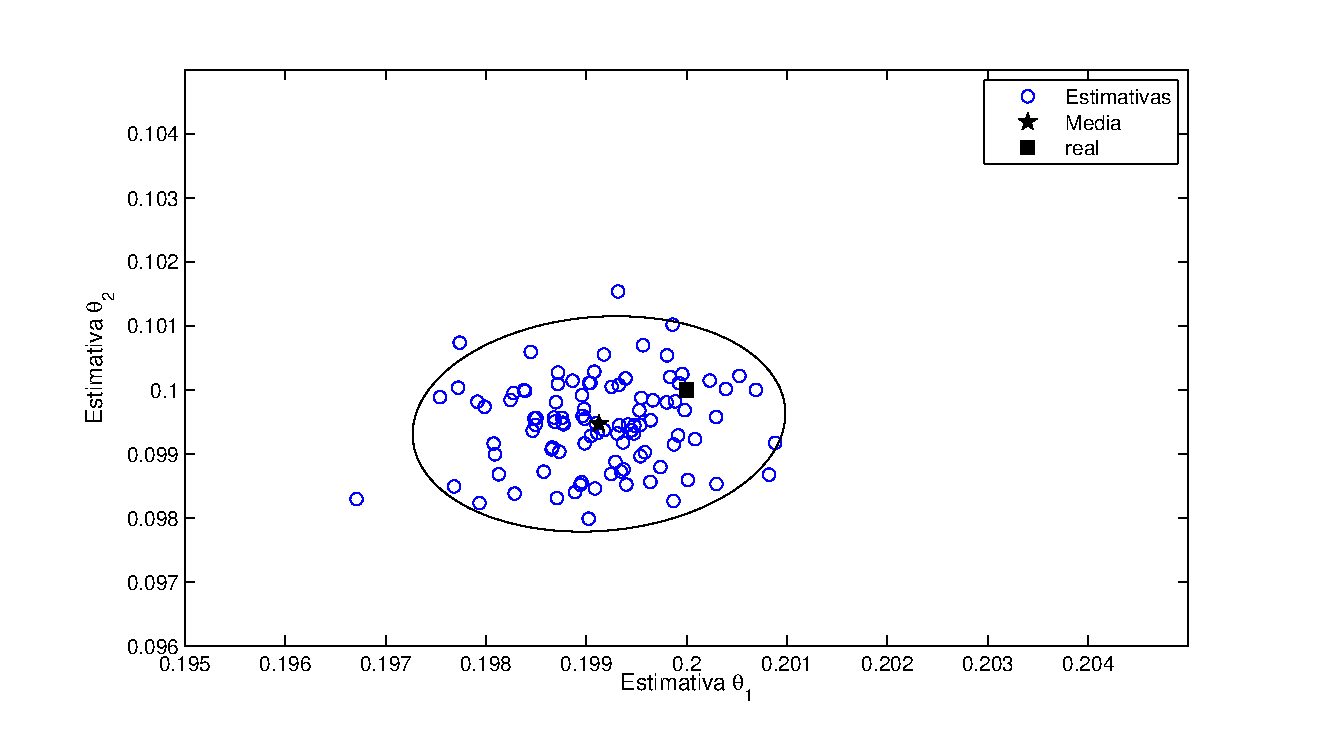
\includegraphics[width=0.9\columnwidth]{figures/rat_example2_a1_a2.eps}
	\caption{Estimativas obtidas nos 100 experimentos de Monte Carlo realizados para as vari�veis $\theta_1$ e
	$\theta_2$.}
	\label{fig:nl_rat_example2}
\end{figure}

%===============================================================================
\subsubsection{Sistemas originalmente racionais, quando $\mathcal{S} \notin \mathcal{M}$}
\label{sec:nl_si_algorithms_rationals_ex2}
%===============================================================================

O sistema descrito abaixo ser� utilizado para a simula��o: 

\begin{equation}
y(t)=\frac{\theta_1y(t-1)+\theta_2y(t-1)u(t-1)+\theta_3u(t-1)}{1+\theta_4y^{2}(t-1)+\theta_5y^{2}(t-2)}
\label{eq:nl_rat_exemple3}
\end{equation}

Para o sistema real utilizou-se os valores de refer�ncia:

\begin{equation}
\theta = 
\begin{bmatrix}
0.2 & 0.1 & 1 & 1 & 1
\end{bmatrix}
\nonumber
\end{equation}


Escolheu-se um modelo que n�o consegue representar totalmente o comportamento do sistema \eqref{eq:nl_rat_exemple3}:

\begin{equation}
y(t)=\frac{\theta_1y(t-1)+\theta_2u(t-1)}{1+\theta_3y^{2}(t-1)+\theta_4y^{2}(t-2)}
\label{eq:nl_rat_exemple3_model}
\end{equation}

Utilizando par a simula��o um sinal PRBS de 635 pontos e um ru�do de vari�ncia $\sigma^2=0.005$ os resultados
da m�dia de 100 estimativas de Monte Carlo foram:

\begin{equation}
\theta_{\text{m�dia}} =\begin{bmatrix}
0.2279  &  1.1341  &  1.2716  &  1.3769
\end{bmatrix}
\nonumber
\end{equation}

A vari�ncia encontrada foi de:

\begin{equation}
\theta+{\text{vari�ncia}} =1.0\times 10^{-3} \begin{bmatrix}
0.0020  &  0.0535  &  0.3402  &	  0.3217
\end{bmatrix}
\nonumber
\end{equation}

A fim de comparar a qualidade dos resultados obtidos, na Figura (\ref{fig:nl_rat_example3}) � apresentado a resposta do
sistema real \eqref{eq:nl_rat_exemple3} e o sistema obtido pela estimativa utilizando o a classe de modelos
\eqref{eq:nl_rat_exemple3_model} para uma entrada do tipo degrau unit�rio.

\begin{figure}[htbp]
	\center
	\includegraphics[width=0.9\columnwidth]{figures/rat_example3.eps}
	\caption{Compara��o do sistema real e do sistema estimado do modelo \eqref{eq:nl_rat_exemple3_model}. Comparativo dos
	sistemas para uma entrada do tipo degrau unit�rio.}
	\label{fig:nl_rat_example3}
\end{figure}

O custo obtido para o modelo estimado foi de:

\begin{equation}
V(\theta)=1.1239
\nonumber
\end{equation}

%===============================================================================
\subsubsection{Conversor CC-CC Buck}
\label{sec:nl_si_algorithms_rationals_buck}
% Aguirre 397
% Tese do corr�a - pg 27
%===============================================================================
O conversor de corrente continua do tipo Buck possui um mapa que pode ser obtido a partir da equa��o do
circuito que tem a forma como em \eqref{eq:nl_alg_buck_circ}. O circuito do
conversor � apresentado na Figura (\ref{fig:nl_models_buck_circuit}). \cite{tse_buck}

\begin{equation}
y(t)=\alpha y(t-1)+\frac{h(d_n)^2 \beta E\left [ E-y(t-1) \right ]}{y(t-1)}
\label{eq:nl_alg_buck_circ}
\end{equation}

Sendo $\alpha = 0.8872$, $\beta = 1.2$ e $E=33$ constantes que dependem apenas dos componentes do
circuito eletr�nico. $d_n$ � um sinal de tens�o que implementa a a��o de controle e a satura��o
$h(d_n)$ � dada por :

\begin{equation}
h(d_n)=\left\{\begin{matrix}
0 & \text{se } d_n < 0\\ 
1 & \text{se } d_n > 1\\ 
d_n & \text{caso contrario.}
\end{matrix}\right.
\nonumber
\end{equation}

\begin{figure}[htbp]
	\center
	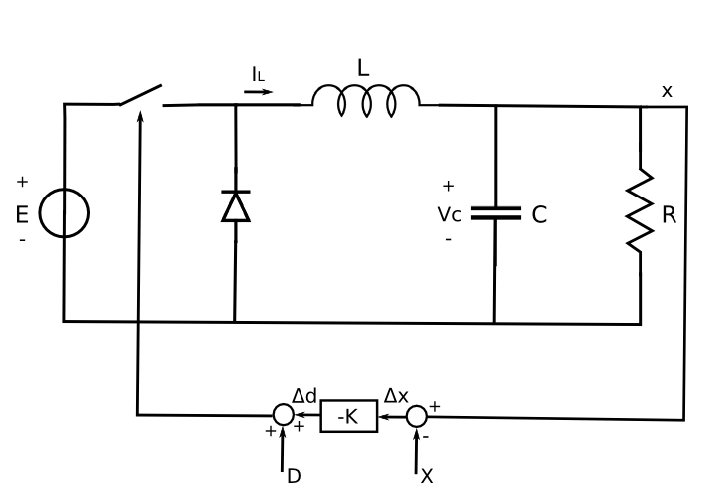
\includegraphics[width=0.55\columnwidth]{figures/nl_models_buck_circuit.eps}
	\caption{Circuito do conversor CC-CC Buck}
	\label{fig:nl_models_buck_circuit}
\end{figure}

Modelos polinomiais n�o resultam em bons modelos para a din�mica de \eqref{eq:nl_alg_buck_circ}. Um
modelo com estrutura {\it{ad rock}}, que aproxima relativamente bem a caracter�stica est�tica do
conversor �: \cite{aguirre_maps}

\begin{equation}
y(t)=O exp\left [ 22-y(t-1) \right ]+ \frac{a\; y(t-1)^2 -b\; y(t-1)+c}{y(t-1)}
\nonumber
\end{equation}

Onde $O=46.429$, $a=2.6204$, $b=99.875$ e $c=1.4171\times 10^3$. Por outro lado a 

Para aplicar o algoritmo, escolhe-se inicialmente um modelo para o sistema em an�lise. O modelo
racional \eqref{eq:nl_alg_buck_rational} aproxima bem a din�mica em quest�o.

\begin{equation}
y(t)=\frac{8.658+0.1223\times10^{-2}y(t-1)^3-0.441\times10^{-1}y(t-1)^2}
{1-0.8381\times10^{-1}y(t-1)+0.1766\times10^{-2}y(t-1)^2}
\label{eq:nl_alg_buck_rational}
\end{equation}

Tendo o modelo escolhido � poss�vel aplicar o algoritmo apresentado na se��o
(\ref{sec:nl_si_algorithms_rationals}). 

Os par�metros da equa��o \eqref{eq:nl_alg_buck_rational} s�o os valores de refer�ncia para a utiliza��o do
m�todos descrito em \cite{aguirre}. Utilizando o algoritmo previamente apresentado, o resultado da estimativa
foi:

\begin{equation}
\theta =\begin{bmatrix}
8.8807 & 8.6698\times 10^{-4} &-0.0359 &-0.0736 & 0.0013 
\end{bmatrix}
\nonumber
\end{equation}

Como pode ser observado, pelos resultados de $\theta$ obtidos e os valores esperados, existe polariza��o na
estimativa obtida. Isso em parte se d� pela falta de capacidade da classe de modelos escolhida em representar
o processo real e pela escolha do modelo de ru�do que para este caso foi apenas utilizado o erro da
estimativa, com rela��o a sa�da do sistema real obtido.

Foram utilizadas amostras de 100 pontos para esta estimativa e realizados 100 experimentos de Monte Carlo.
Os resultados obtidos foram de uma m�dia de:

\begin{equation}
\text{m�dia de }\;\theta =\begin{bmatrix}
8.8976  &    8.6762\times 10^{-4}    & -0.0360 &  -0.0736  &  0.0013
\end{bmatrix}
\nonumber
\end{equation}

e uma vari�ncia de

\begin{equation}
\theta_{\text{vari�ncia}} =\begin{bmatrix}
0.4842\times 10^{-3}  \\ 1.8004\times 10^{-12} \\ 3.5416\times 10^{-9} \\ 1.9850\times 10^{-9} \\ 2.4100\times
10^{-12}
\end{bmatrix}^T
\nonumber
\end{equation}

com uma covari�ncia de 

\begin{equation}
\theta_{\text{Covari�ncia}} = 1.0\times 10^{-3}\begin{bmatrix}
 0.4842 &  0.0000 & -0.0011 &  0.0007 &-0.0000 \\
 0.0000 &  0.0000 & -0.0000 & -0.0000 & 0.0000 \\
-0.0011 & -0.0000 &  0.0000 & -0.0000 & 0.0000 \\
 0.0007 & -0.0000 & -0.0000 &  0.0000 &-0.0000 \\
-0.0000 &  0.0000 &  0.0000 & -0.0000 & 0.0000 
\end{bmatrix}
\nonumber
\end{equation}


%===============================================================================
\section{Considera��es Finais}
\label{sec:nl_conclusions}
%===============================================================================

Neste cap�tulo apresentou-se conceitos b�sicos de identifica��o de sistemas n�o lineares. Inicialmente foram
apresentados os tipos de linearidades existentes. Muitas vezes os sistemas comportam-se de forma linear entorno da
regi�o de opera��o do sistema, desta forma identificar um sistema com um modelo linear � o que normalmente se utiliza.
Para os casos onde h� necessidade de modelar a din�mica n�o linear, ou que se deseja modelar caracter�sticas
espec�ficas do sistema, uma classe de modelos n�o linear � mais apropriado.

Apresentou-se alguns dos conjuntos de modelos mais utilizados para identifica��o de sistemas n�o lineares de tempo
discreto e algumas de suas caracter�sticas. Destacou-se que a escolha de um modelo em detrimento de outro � um aspecto
muito importante para a identifica��o de sistemas n�o lineares. A escolha de uma base e a ordem do modelo s�o muito
importantes para que n�o sejam acrescidos ao modelo din�micas que n�o existem no sistema real.

Deu-se especial aten��o a classe de modelos NARMAX em suas duas formas mais conhecidas: polinomial e racional. Estes
conjuntos de modelos conseguem representar uma grande variedade de sistemas n�o lineares utilizando uma estrutura
simples de compreender e que por ser linear nos par�metros, faz com que os algoritmos para a identifica��o
de seus par�metros sejam mais simples.

Apresentou-se um algoritmo para identifica��o de modelos racionais, que pode ser utilizado para modelos
polinomiais sem dificuldades. Este algoritmo iterativo obteve bons resultados para os experimentos efetuados e estes
resultados foram apresentados para diversos tipos de classes de modelos escolhidas.

Observou-se o desempenho deste algoritmo para situa��es onde a classe de modelo do sistema consegue representar
totalmente o sistema real sob an�lise ($\mathcal{S} \in \mathcal{M}$), situa��o onde isso n�o � verdade ($\mathcal{S}
\notin \mathcal{M}$).

O algoritmo implementado n�o contemplou a modelagem do ru�do do sistema, sendo este um aspecto para ser desenvolvido em
trabalhos futuros, visto que este fato � bastante importante para situa��es onde $\mathcal{S} \notin \mathcal{M}$,
podendo o algoritmo nestas situa��es convergir para pontos onde os par�metros identificados n�o sejam os reais. esta
situa��o foi apresentada no exemplo do conversor de corrente continua do tipo Buck (Se��o
\ref{sec:nl_si_algorithms_rationals_buck}).



%===============================================================================


%===============================================================================
\chapter{Controle baseado em dados}
\label{chapter:dbcd}
%===============================================================================

Este cap�tulo tem como objetivo introduzir o conceito de projeto de controladores baseados em dados, introduzir alguns
dos principais metodos existentes e dar enf�se maior ao metodo {\it{Virtual reference feedback tuning}} - VRFT
que utiliza refer�ncia virtual como uma de suas bases.

Inicialmente na se��o \ref{sec:dbcd_definition} ser� introduzido o conceito de projeto de controlaodres baseados
em dados. Alguns dos principais m�todos e suas subdivis�es em m�todos diretos: onde n�o existe a necessidade de
identifica��o da planta, para ent�o identificar o controlador; m�todos iterativos: onde a cada conjunto de dados
coletados da planta um novo controlador � encontrado e aplicado sobre a planta at� que se convirja para o valor m�nimo
da fun��o custo.

Deseja-se adicionar um enfoque ao m�todo direto que utiliza refer�ncia virtual: VRFT (se��o \ref{sec:dbcd_vrft}).
Quer-se com isso introduzir e exeplificar a utiliza��o de refer�ncia virtual para a obten��o dos sinais necess�rios para
a identifica��o do controlador ideal para este sistema.

Ao fim, na se��o \ref{sec:dbcd_conclusions}, ser�o apresentadas as considera��es finais a respeito do que foi visto
neste capitulo.

%===============================================================================
%===============================================================================
\section{Defini��es}
\label{sec:dbcd_definition}
%===============================================================================
O projeto de controladores baseados em dados consiste em obter, ou estimar, os par�metros de uma fam�lia ou conjunto de 
modelos baseados nos dados obtidos da planta sob an�lise. Os dados utilizados para esta tarefa s�o usualmente os sinais
de entrada e sa�da do sistema.

Como j� foi discutido na se��o (\ref{sec:si_project_experiments}) estes dados podem ser obtidos de
diversas formas. Algumas vezes estas informa��es podem vir da opera��o normal da planta em malha
fechada com a presen�a de algum controlador. Situa��o esta que tem um grande apelo em plantas
industriais, onde a parada do processo, para levantamento de informa��es, � indesej�vel e muitas
vezes at� invi�vel. Se existe a possibilidade de parar a planta e aplicar sinais predeterminados,
o projeto de experimentos pode trazer muitas vantagens (se��o \ref{sec:si_project_experiments}).

O projeto de controladores baseados em dados consiste em estimar os parametros da estrutura do controlador usando os
dados de entrada e sa�da coletados do sistema. A estimativa � feita de forma direta, ou seja, sem a necessidade de um
passo intermedi�rio para identifica��o da planta do processo. \cite{eckard_campestrini}

% http://www.sciencedirect.com/science/article/pii/S0005109808002288
% Several data-based control design methods explicitly optimizing performance criteria have appeared in the
% literature, with different approaches and for different performance criteria. These criteria express either one or a combination  of
% the fundamental control objectives: reference tracking, noise rejection, and economic use of control energy. In Kammer,
% Bitmead, and Bartlett (2000) an iterative procedure based on spectral analysis, named Frequency Domain Tuning (FDT), 
% has been proposed for the minimization of an H2 performance criterion for a system with zero reference; hence, no
% tracking objective is pursued. The Virtual Reference Feedback Tuning (VRFT) method ( [Campi et al., 2002] and [Campi
% and Savaresi, 2006]) is based on a clever manipulation of variables which transforms an H2 performance criterion into
% one which is quadratic in the design parameters. The resulting quadratic cost function can be minimized directly, so
% that no iterations are required. However, only the reference tracking objective is treated (unless a two degree of
% freedom controller is used, as in Lecchini, Campi, and Savaresi (2002)) and the global minimum of the resulting
% quadratic function coincides with that of the original criterion only under ideal conditions. Not suffering from this
% second limitation, but again an iterative procedure, is Correlation-based Tuning (CbT) ( [Karimi et al., 2003] and
% [Karimi et al., 2004]), which uses instrumental variable ideas to eliminate the deleterious effect of noise on the
% achievement of its reference tracking objective. Data-based optimization of a general H2 performance criterion appears
% in Hjalmarsson, Gunnarsson, and Gevers (1994). There, a method for obtaining an unbiased estimate of the gradient of
% the cost function directly from closed-loop data is proposed; this method has been named Iterative Feedback Tuning
% (IFT). IFT is discussed in depth in Hjalmarsson, Gevers, Gunnarsson, and Lequin (1998), Hjalmarsson (2002) and
% extended in Proch�zka, Gevers, Anderson, and Ferrera (2005) to even more general performance criteria, which contain
% robustness enhancement objectives.
 
Existem na literatura diversos m�todos de projetos de controladores baseados em dados que otimizam algum crit�rio de
performance, com diferentes focos para diferentes crit�rios. Estes crit�rios expressam um ou uma combina��o de objetivos
fundamentais de controle: seguimento de refer�ncia, rejei��o a ru�do e uso economico da energia de controle.
Em \cite{Kammer2000} um procedimento iterativo baseado na an�lise espectral chamado de {\it{Frequency Domain Tuning}}
(FDT) foi proposto para a minimiza��o do crit�rio $H_2$ de performance para um sistema com refer�ncia zero, portanto
sem nenhum objetivo de seguimento de refer�ncia � almejado. O m�todo {\it{Virtual Reference Feedback Tuning}} (VRFT)
\cite{campi_leccini_savaresi2002, campi_savaresi2006} � baseado na manipula��o de vari�veis que transformam um
crit�rio $H_2$ em algo quadr�tico nos parametros. A fun��o custo quadr�tica resultante pode ser minimizado
diretamente, sem que nenhuma itera��o seja necess�ria. Entretanto apenas o objetivo de seguimento de refer�ncia �
tratato (a n�o ser que um controlador com dois n�veis de liberdade seja usado \cite{lecchini_campi_savaresi_2dof}) e o minimo
global resultante desta fun��o quadr�ica coincide com o do crit�rio original somente sob condi��es ideais.
{\it{Correlation-based Tuning}} (CbT) \cite{ Karimi_cbt2003, Karimi_cbt2004} n�o sofre desta segunda limita��o, mas �
um m�todo iterativo que usa a ideia de vari�veis instrumentais para remover o efeito indesejado do ru�do enquanto
busca seu objetivo de seguimento de refer�ncia. \cite{Bazanella_h2criteria2008} 

Otimiza��o baseada em dados para um crit�rio de performance gen�rico $H_2$ foi proposto em \cite{Hjalmarsson1994}, onde
um m�todo para obter estimativas n�o polarizadas diretamente do gradiente da fun��o custo apartir de dados do sistema em
malha fechada foi elaborado. Este m�todo � chamado de {\it{Iterative Feedback Tuning}} (IFT). IFT � discutido a fundo em
\cite{Hjalmarsson_ift1998, Hjalmarsson2002} e extendido em \cite{Prochazka2005} para crit�rio de performances mais
gerais, que cont�m melhorias em objetivos de robustes. \cite{Bazanella_h2criteria2008} 

Seja a esperan�a de um valor $E\left [ \cdot \right ]$ definido por: \cite{ljung}

\begin{equation}
\bar{E}\left [ f(t) \right ]\equiv \lim_{N \to \infty } \frac{1}{N}\sum_{t=1}^{N}E\left [ f(t)
\right]
\label{eq:vrft_db_hope}
\end{equation}

O ru�do � um processo quasi-estacion�rio, que pode ser descrito como $\nu(t)=H_0(z)e(t)$, onde
$e(t)$ � ru�do branco com vari�ncia $\sigma_e^2(t)$. Ambas fun��es de transfer�ncia, $G_0(z)$ e $H_0(z)$,
s�o racionais e causais. Assume-se que $H(\infty)=1$, ou seja, a resposta impulsiva do filtro
$H_0(z)$ satisfaz $h(0)=1$. \cite{campestrini}

Na Figura (\ref{fig:vrft_db_control_loop}) � apresentado um usual sistema com realimenta��o de sa�da onde s�o
destacados os blocos do controlador, da planta e da fun�a� que modifica o ru�do branco $e(t)$.

\begin{figure}[htbp]
\center
% Generated with LaTeXDraw 2.0.8
% Tue Jun 05 22:30:25 BRT 2012
% \usepackage[usenames,dvipsnames]{pstricks}
% \usepackage{epsfig}
% \usepackage{pst-grad} % For gradients
% \usepackage{pst-plot} % For axes
\scalebox{1} % Change this value to rescale the drawing.
{
\begin{pspicture}(0,-2.0492187)(9.84,2.0692186)
\pscircle[linewidth=0.04,dimen=outer](1.401875,-1.0292188){0.2}
\psframe[linewidth=0.04,dimen=outer](4.401875,-0.62921876)(2.601875,-1.4292188)
\psframe[linewidth=0.04,dimen=outer](7.201875,-0.62921876)(5.601875,-1.4292188)
\pscircle[linewidth=0.04,dimen=outer](8.401875,-1.0292188){0.2}
\psline[linewidth=0.04cm,arrowsize=0.05291667cm 2.0,arrowlength=1.4,arrowinset=0.4]{->}(0.001875,-1.0292188)(1.201875,-1.0292188)
\psline[linewidth=0.04cm,arrowsize=0.05291667cm 2.0,arrowlength=1.4,arrowinset=0.4]{->}(1.601875,-1.0292188)(2.601875,-1.0292188)
\psline[linewidth=0.04cm,arrowsize=0.05291667cm 2.0,arrowlength=1.4,arrowinset=0.4]{->}(4.401875,-1.0292188)(5.601875,-1.0292188)
\psline[linewidth=0.04cm,arrowsize=0.05291667cm 2.0,arrowlength=1.4,arrowinset=0.4]{->}(7.201875,-1.0292188)(8.201875,-1.0292188)
\psline[linewidth=0.04cm,arrowsize=0.05291667cm 2.0,arrowlength=1.4,arrowinset=0.4]{->}(8.4,0.16921872)(8.401875,-0.82921875)
\psline[linewidth=0.04cm,arrowsize=0.05291667cm 2.0,arrowlength=1.4,arrowinset=0.4]{->}(8.601875,-1.0292188)(9.801875,-1.0292188)
\psline[linewidth=0.04cm,arrowsize=0.05291667cm 2.0,arrowlength=1.4,arrowinset=0.4]{<-}(1.401875,-1.2292187)(1.401875,-2.0292187)
\psline[linewidth=0.04cm](1.401875,-2.0292187)(9.201875,-2.0292187)
\psline[linewidth=0.04cm](9.201875,-2.0292187)(9.201875,-1.0292188)
\usefont{T1}{ptm}{m}{n}
\rput(1.0771874,-0.7192188){+}
\usefont{T1}{ptm}{m}{n}
\rput(8.0771885,-0.7192188){+}
\usefont{T1}{ptm}{m}{n}
\rput(8.0771885,-1.3192188){+}
\usefont{T1}{ptm}{m}{n}
\rput(1.6265626,-1.3192188){-}
\usefont{T1}{ptm}{m}{n}
\rput(0.441875,-0.7292188){\small $r(t)$}
\usefont{T1}{ptm}{m}{n}
\rput(3.561875,-1.0292188){\small $C(z, \rho)$}
\usefont{T1}{ptm}{m}{n}
\rput(6.331875,-1.0492188){\small $G_0(z)$}
\usefont{T1}{ptm}{m}{n}
\rput(5.081875,-0.7292188){\small $u(t)$}
\usefont{T1}{ptm}{m}{n}
\rput(1.941875,-0.7292188){\small $\varepsilon (t)$}
\usefont{T1}{ptm}{m}{n}
\rput(7.851875,-0.20921877){\small $\nu(t)$}
\usefont{T1}{ptm}{m}{n}
\rput(9.271875,-0.7292188){\small $y(t)$}
\psframe[linewidth=0.04,dimen=outer](9.201875,0.9707812)(7.601875,0.17078124)
\usefont{T1}{ptm}{m}{n}
\rput(8.331875,0.55078125){\small $H_0(z)$}
\psline[linewidth=0.04cm](8.4,0.96921873)(8.4,1.5692188)
\usefont{T1}{ptm}{m}{n}
\rput(8.271875,1.8707812){\small $e(t)$}
\end{pspicture} 
}
\caption{Sistema de controle em malha fechada, com presen�a do sinal de ru�do.}
\label{fig:vrft_db_control_loop}
\end{figure}

A equa��o \eqref{eq:vrft_db_closed_loop} descreve a rela��o entre entrada e sa�da do sistema
apresentado na Figura (\ref{fig:vrft_db_control_loop}).

\begin{equation}
T(z, \rho)=\frac{C(z,\rho)G_0(z)}{1+C(z,\rho)G_0(z)}
\label{eq:vrft_db_closed_loop}
\end{equation}

projeto de controladires baseados em dados podem ser divididos em dois grupos principais: m�todos iterativos onde
experimentos s�o realizados sobre o sistema atualizando-se o controlador a cada itera��o, repete-se o processo  at� que
se atinja um valor minimo para a fun��o custo. O segundo grupo � o de m�todos n�o iterativos, onde apenas com um
experimento, ou um conjunto de dados, os par�metros do controlador s�o estimados.

%===============================================================================
\subsection{Iterative feedback tuning}
\label{sec:vrft_control_ift}
%===============================================================================

O m�todo IFT utiliza um algoritmo iterativo para minimizar uma fun��o custo $H_2$. O m�todo
considera que o sistema � controlado por um controlador com dois graus de liberdade:

\begin{equation}
u(t)=C_r(z)r(t)-C_y(z)y(t)
\label{eq:vrft_db_ift_controller}
\end{equation}

Na Figura (\ref{fig:vrft_db_ift}) � apresentado a organiza��o dos blocos dos controladores
de \eqref{eq:vrft_db_ift_controller}, $C_r(z)$ e $C_y(z)$. O controlador pode ser
entendido como o conjunto destes dois:\cite{Hjalmarsson_ift1998}

\begin{equation}
C(z) \equiv  \left \{ C_r(z),\, C_y(z)  \right \} 
\nonumber
\end{equation}

\begin{figure}[htbp]
\center
\scalebox{1} % Change this value to rescale the drawing.
{
\begin{pspicture}(0,-1.68)(9.48,1.72)
\usefont{T1}{ptm}{m}{n}
\rput(7.691875,1.5215625){\small $\nu(t)$}
\pscircle[linewidth=0.04,dimen=outer](4.0,0.32){0.2}
\pscircle[linewidth=0.04,dimen=outer](8.0,0.32){0.2}
\psframe[linewidth=0.04,dimen=outer](6.8,0.72)(5.2,-0.08)
\psframe[linewidth=0.04,dimen=outer](2.8,0.72)(1.2,-0.08)
\psframe[linewidth=0.04,dimen=outer](6.8,-0.88)(5.2,-1.68)
\psline[linewidth=0.04cm,arrowsize=0.05291667cm 2.0,arrowlength=1.4,arrowinset=0.4]{->}(0.0,0.32)(1.2,0.32)
\psline[linewidth=0.04cm,arrowsize=0.05291667cm 2.0,arrowlength=1.4,arrowinset=0.4]{->}(2.8,0.32)(3.8,0.32)
\psline[linewidth=0.04cm,arrowsize=0.05291667cm 2.0,arrowlength=1.4,arrowinset=0.4]{->}(4.2,0.32)(5.2,0.32)
\psline[linewidth=0.04cm,arrowsize=0.05291667cm 2.0,arrowlength=1.4,arrowinset=0.4]{->}(6.8,0.32)(7.8,0.32)
\psline[linewidth=0.04cm,arrowsize=0.05291667cm 2.0,arrowlength=1.4,arrowinset=0.4]{->}(8.2,0.32)(9.2,0.32)
\psline[linewidth=0.04cm,arrowsize=0.05291667cm 2.0,arrowlength=1.4,arrowinset=0.4]{<-}(6.8,-1.28)(8.0,-1.28)
\psline[linewidth=0.04cm](8.0,-1.28)(8.0,0.12)
\psline[linewidth=0.04cm,arrowsize=0.05291667cm 2.0,arrowlength=1.4,arrowinset=0.4]{<-}(4.0,0.12)(4.0,-1.28)
\psline[linewidth=0.04cm](4.0,-1.28)(5.2,-1.28)
\usefont{T1}{ptm}{m}{n}
\rput(8.911875,0.5215625){\small $y(t)$}
\usefont{T1}{ptm}{m}{n}
\rput(0.481875,0.5215625){\small $r(t)$}
\usefont{T1}{ptm}{m}{n}
\rput(1.901875,0.3215625){\small $C_r(z)$}
\usefont{T1}{ptm}{m}{n}
\rput(5.951875,0.3215625){\small $G_0(z)$}
\usefont{T1}{ptm}{m}{n}
\rput(5.931875,-1.2784375){\small $C_y(z)$}
\usefont{T1}{ptm}{m}{n}
\rput(4.721875,0.7215625){\small $u(t)$}
\psline[linewidth=0.04cm,arrowsize=0.05291667cm 2.0,arrowlength=1.4,arrowinset=0.4]{->}(8.0,1.32)(8.0,0.52)
\usefont{T1}{ptm}{m}{n}
\rput(4.2592187,0.1315625){-}
\end{pspicture} 
}
\caption{Diagrama de bloco do sistema utilizado na identifica��o IFT.}
\label{fig:vrft_db_ift}
\end{figure}

A fun��o custo utilizada como crit�rio no m�todo � apresentada em \eqref{eq:vrft_db_ift_j_cost}. 

\begin{equation}
J(\rho)=\frac{1}{2N}E\left [ \sum_{t=1}^{N}(L_y \tilde{y}_t(\rho))^2 +\lambda  \sum_{t=1}^{N}(L_u
u_t(\rho))^2 \right ]
\label{eq:vrft_db_ift_j_cost}
\end{equation}

O primeiro termo em \eqref{eq:vrft_db_ift_j_cost} � o erro entre a resposta obtida e a resposta
desejada, balanceada por um filtro $L_y$ a segunda parte � o custo de controle balanceado pelo
filtro $L_u$. Com $T_0(\rho)$ e $S_0(\rho)$ sendo a fun��o de transfer�ncia em malha fechada e a
fun��o sensibilidade, respectivamente:


\begin{equation}
T_0(\rho)=\frac{C_r(\rho)G_0}{1+C_y(\rho)G_0}
\nonumber
\end{equation}

\begin{equation}
S_0(\rho)=\frac{1}{1+C_y(\rho)G_0}
\nonumber
\end{equation}

E sendo $r$ e $\nu$ independentes, \eqref{eq:vrft_db_ift_j_cost} pode ser rescrito como
\eqref{eq:vrft_db_ift_j_cost_parts}

\begin{equation}
J(\rho)=\frac{1}{2N}\sum_{t=1}^{N}\left \{ L_y(T_d r-T_0(\rho)r) \right \}^2+\frac{1}{2} E\left [ \left \{ L_y S_0(\rho) \nu \right \}^2 \right ]
+ \lambda \frac{1}{2N}E\left [ \sum_{t=1}^{N}(L_u u_t(\rho))^2 \right ]
\label{eq:vrft_db_ift_j_cost_parts}
\end{equation}

Onde o primeiro termo � o erro de seguimento de refer�ncia, o segundo � a contribui��o do dist�rbio
e o terceiro � o esfor�o de controle.

Para minimizar \eqref{eq:vrft_db_ift_j_cost_parts}, busca-se encontrar um ponto
estacion�rio da equa��o, para isso calcula-se o gradiente desta equa��o e aplica-se o
algoritmo para a converg�ncia apresentado em \eqref{eq:vrft_db_ift_algoritm}.
\cite{hajalmson_ift_non_linear}

\begin{equation}
\rho_{i+1}=\rho_i - \gamma_i R_i^{-1}\frac{\partial J}{\partial \rho}(\rho_i)
\label{eq:vrft_db_ift_algoritm}
\end{equation}

$R_i$ � uma matriz positiva definida, tipicamente uma estimativa da Hessiana de $J$, como por
exemplo a aproxima��o de Gauss-Newton.

Para cada itera��o $i$ em \eqref{eq:vrft_db_ift_algoritm}, o m�todo IFT necessita de dois
experimentos, cada um de tamanho $N$. 


% ===============================================================================
\section{Virtual reference feedback tuning}
\label{sec:dbcd_vrft}
% ===============================================================================

% Em aplica��es pr�ticas, a descri��o matem�tica da planta n�o � dispon�vel e o sistema deve ser identificado
% baseado nas medidas obtidas deste sistema. Este assunto tem atra�do a aten��o de diversos engenheiros de
% controle desde 1940 com o pioneiro trabalho de Ziegler e Nichols (1942) com ajuste de controladores PID
% industriais. Depois do trabalho de Ziegler e Nichols diversos trabalhos surgiram, muitos em formas de
% aperfei�oamento e extens�es das t�cnicas j� apresentadas, e algumas com desenvolvimentos em novas dire��es
% (\cite{mcmillan1983tuning}, \cite{Haalman1965}). A caracter�stica principal destes m�todos � que eles podem
% ser facilmente utilizados: simples experimentos sobre a planta s�o executados e simples regras 
% s�o aplicadas sobre os dados obtidos. \cite{campi_leccini_savaresi2002}


VRFT do ingl�s {\it{Virtual reference feedback tuning}} � um m�todo direto para identifica��o de
controladores, ou seja, n�o � necess�rio o conhecimento ou identifica��o da planta para que este m�todo seja
utilizado. O m�todo se baseia na utiliza��o de apenas um conjunto de dados, n�o necessitando de experimentos
espec�ficos. O procedimento procura pelo ponto �timo do crit�rio escolhido para a identifica��o do controlador.
\cite{campi_savaresi2000}

Diferentemente de m�todos iterativos, o VRFT n�o recai sobre m�nimos locais, sempre procurando o m�nimo
global do crit�rio escolhido, sob condi��es ideais:

\begin{itemize}
  \item O sistema n�o � afetado por ru�do, ou seja, $\sigma_e^2(t)=0$.
  \item O controlador ideal $C_d(z) \in C(z, \theta)$.
  \item O controlador � parametrizado linearmente. 
\end{itemize}

O controlador a ser identificado pode ser parametrizado como abaixo:

\begin{equation}
C(z,\theta)=\beta^T(z)\theta
\label{eq:vrft_method_controller}
\end{equation}
onde $\beta(z) = \left [ \beta_1(z)\;\; \beta_2(z)\;\; \cdots \;\; \beta_n(z)\right ]^T$ � um vetor
linear de fun��es de transfer�ncias de tempo discreto e $\theta$ � o vetor de par�metros a ser estimado.

O problema de identifica��o do controlador consiste em encontrar um $\hat{\theta}$ que minimize o
crit�rio performance \eqref{eq:dbcd_def_track_error}, replicado abaixo:

\begin{equation}
J_y(\theta)\overset{\underset{\mathrm{\Delta}}{\,}}{=}  \bar{E} \left [ y(t)-y_d(t) \right ]^2 = \bar{E}\left [
(T(z,\theta)-T_d(z))r(t) \right ]^2
\nonumber
\end{equation}
que � dependente do modelo de refer�ncia escolhido. 

Apenas alguns m�todos genuinamente diretos s�o encontrados na literatura, dois destes s�o VRFT e IFT. Mesmo
estes dois m�todos pertencendo uma a mesma classe, algumas difer�n�as significativas existem e podem ser ressaltadas:
\cite{campi_savaresi2000}

\begin{itemize}
	\item {\it{IFT}} � baseado em um m�todos de gradiente decrescente e al�m disso � uma t�cnica
	iterativa. Usualmente este m�todo converge para o m�nimo local mais pr�ximo das condi��es iniciais.
	Ele requer experimentos espec�ficos sobre a planta, com entradas espec�ficas.
	\item {\it{VRFT}} � um procedimento n�o iterativo que procura pelo m�nimo global do crit�rio de
	performance \eqref{eq:dbcd_def_track_error}. Este m�todo n�o requer experimentos espec�ficos sobre
	a planta, podendo inclusive utilizar os dados do funcionamento normal do sistema.
\end{itemize}

%===============================================================================
\subsection{O m�todo}
\label{sec:dbcd_vrft_framework}
%===============================================================================

Nesta se��o ser� apresentado uma breve descri��o de como funciona o algoritmo para obten��o do controlador
utilizando o m�todo VRFT. Para maiores detalhes e discuss�es aprofundadas � indicada a leitura de
\cite{campi_savaresi2000, campi_leccini_savaresi2002, campestrini_nonminumum_phase, bazanella_datadriven}.

Suponha que o controlador $C(z, \theta)$ resulta um sistema em malha fechada cuja fun��o de
transfer�ncia � dada por $T_d(z)$. Desta forma, se $T_d(z)$ for excitado com qualquer sinal $r(t)$,
sua sa�da ser� $T_d(z)r(t)$. Uma premissa para que o sistema em malha fechada tenha a mesma
fun��o de transfer�ncia que o modelo de refer�ncia � que a sa�da dos dois sejaM a mesma para um dado
sinal $\bar{r}(t)$.

Baseado no sinal medido $y(t)$, considera-se um sinal $\bar{r}(t)$ tal que $T_d(z)\bar{r}(t)=y(t)$.
Esta refer�ncia � conhecida como {\it{virtual}} pois ela n�o existe e n�o foi utilizada para gerar o
sinal $y(t)$. A figura (\ref{fig:vrft_method_cl}) apresenta o sistema em malha fechada e os sinais
presentes.

\begin{figure}[htbp]
\center
%\scalebox{1} % Change this value to rescale the drawing.
%{
\begin{pspicture}(0,-1.4292188)(9.02,1.4692187)
\pscircle[linewidth=0.04,linestyle=dashed,dash=0.16cm 0.16cm,dimen=outer](1.4,0.97078127){0.2}
\psframe[linewidth=0.04,linestyle=dashed,dash=0.16cm 0.16cm,dimen=outer](4.8,1.3707813)(3.0,0.57078123)
\psframe[linewidth=0.04,dimen=outer](7.6,1.3707813)(6.0,0.57078123)
\psline[linewidth=0.04cm,arrowsize=0.05291667cm 2.0,arrowlength=1.4,arrowinset=0.4]{->}(0.0,0.97078127)(1.2,0.97078127)
\psline[linewidth=0.04cm,linestyle=dashed,dash=0.16cm 0.16cm,arrowsize=0.05291667cm 2.0,arrowlength=1.4,arrowinset=0.4]{->}(1.6,0.97078127)(3.0,0.97078127)
\psline[linewidth=0.04cm,arrowsize=0.05291667cm 2.0,arrowlength=1.4,arrowinset=0.4]{->}(4.8,0.97078127)(6.0,0.97078127)
\psline[linewidth=0.04cm](7.6,0.97078127)(9.0,0.97078127)
\psline[linewidth=0.04cm,linestyle=dashed,dash=0.16cm 0.16cm,arrowsize=0.05291667cm 2.0,arrowlength=1.4,arrowinset=0.4]{<-}(1.4,0.7707813)(1.4,-0.02921875)
\psline[linewidth=0.04cm,linestyle=dashed,dash=0.16cm 0.16cm](1.4,-0.02921875)(8.4,-0.02921875)
\psline[linewidth=0.04cm,linestyle=dashed,dash=0.16cm 0.16cm](8.4,-0.02921875)(8.4,0.97078127)
\usefont{T1}{ptm}{m}{n}
\rput(1.1126562,1.2807813){+}
\usefont{T1}{ptm}{m}{n}
\rput(1.6473438,0.68078125){-}
\usefont{T1}{ptm}{m}{n}
\rput(0.47,1.2707813){\small $\bar{r}(t)$}
\usefont{T1}{ptm}{m}{n}
\rput(3.99,0.97078127){\small $C(z, \theta)$}
\usefont{T1}{ptm}{m}{n}
\rput(6.76,0.9507812){\small $G_0(z)$}
\usefont{T1}{ptm}{m}{n}
\rput(5.51,1.2707813){\small $u(t)$}
\usefont{T1}{ptm}{m}{n}
\rput(2.25,1.2707813){\small $\varepsilon (t)$}
\usefont{T1}{ptm}{m}{n}
\rput(8.3,1.2707813){\small $y(t)$}
\psframe[linewidth=0.04,dimen=outer](6.0,-0.62921876)(3.8,-1.4292188)
\usefont{T1}{ptm}{m}{n}
\rput(4.91,-1.0492188){\small $T_d^{-1}(z)$}
\psline[linewidth=0.04cm](9.0,0.97078127)(9.0,-1.0292188)
\psline[linewidth=0.04cm](9.0,-1.0292188)(6.0,-1.0292188)
\psline[linewidth=0.04cm](3.8,-1.0292188)(0.0,-1.0292188)
\psline[linewidth=0.04cm](0.0,-1.0292188)(0.0,0.97078127)
\end{pspicture} 
%}
\caption{Diagrama de blocos para o m�todo VRFT. S�o destacados os sinais reais $u(t)$ e $y(t)$ al�m dos sinais virtuais
$\varepsilon (t)$ e $\bar{r}(t)$. Em pontilhado est� o controlador que quando aplicado sobre a malha, faz com que o
sistema se comporte como desejado: $T_d(z)$.}
\label{fig:vrft_method_cl}
\end{figure}

O sinal $\varepsilon(t)$ � o erro entre os sinais $y(t)$ e $\bar{r}(t)$. Sabe-se que quando a planta �
excitada com o sinal $u(t)$, o sinal $y(t)$ � obtido. Analogamente para um controlador, quando este �
excitado com o sinal $\varepsilon(t)$, o sinal $u(t)$ � obtido. A tarefa do m�todo VRFT � encontrar este
controlador, com os sinais $u(t)$ e $\varepsilon(t)$ que s�o conhecidos, a tarefa reduz-se a um problema de
identifica��o. Comumente, usa-se um pr�-filtro nos dados coletados. A ideia principal do uso deste
filtro ser� explicada posteriormente na se��o (\ref{sec:dbcd_vrft_framework_filter}). 

O algoritmo pode ser descrito pelos passos a seguir \cite{campi_savaresi2000}:

\begin{enumerate}
	\item Filtram-se os sinais de entrada e sa�da com algum filtro $L(z)$:

\begin{equation}
y_L (t)=L(z)y(t), \;\;\; u_L (t)=L(z)u(t) 
\label{eq:vrft_method_algorithm_filter_io}
\end{equation}

\begin{equation}
\varepsilon_L (t)=L(z)\varepsilon (t)=\bar{r}_L (t)-y_L (t) 
\nonumber
\end{equation}


\item Encontra-se um sinal de refer�ncia $\bar{r}_L (t)$ no qual a sa�da do modelo de refer�ncia
$T_d(z)$ seja exatamente $y_L (t)$ quando alimentado pelo sinal:

\begin{equation}
y_L (t)=T_d(z) \bar{r}_L (t)
\label{eq:vrft_method_algorithm_ref}
\end{equation}

\item Seleciona-se o vetor de par�metros do controlador $\hat{\theta}$ que minimize o crit�rio:

\begin{equation}
J_{VR}^N(\theta)=\frac{1}{N}\sum_{t=1}^{N}(u_L(t)-\varphi_L^T(t)\theta)^2
\label{eq:vrft_method_algorithm_criter}
\end{equation}

\begin{equation}
\varphi_L(t)=\beta(z)\varepsilon_L(t)
\nonumber
\end{equation}

Desde que \eqref{eq:vrft_method_algorithm_criter} seja quadr�tica em $\theta$ o vetor de par�metros
$\hat{\theta}$ que minimiza esta fun��o custo pode ser calculado por:

\begin{equation}
\hat{\theta}= \left [ \sum_{t=1}^{N}\varphi_L(t) \varphi_L(t)^T\right ]^{-1}
\sum_{t=1}^{N}\varphi_L(t) u_L(t)
\label{eq:vrft_method_algorithm_result}
\end{equation}

\end{enumerate}

Com o int�ito de exemplificar, na Figura (\ref{fig:vrft_cost_functions}) � apresentado uma curva da fun��o custo
$J_y(\theta)$ de um sistema hipot�tico, e a fun��o custo proposta pelo m�todo VRFT $J_{VR}(\theta)$, a qual � quadr�tica em $\theta$.
Ao tentar encontrar o ponto de m�nimo da curva $J_y(\theta)$ pode-se recair em algum m�nimo local, o que n�o acontece 
para a curva  $J_{VR}(\theta)$.

\begin{figure}[htbp]
\center
% Generated with LaTeXDraw 2.0.8
% Mon Jul 02 22:05:15 BRT 2012
% \usepackage[usenames,dvipsnames]{pstricks}
% \usepackage{epsfig}
% \usepackage{pst-grad} % For gradients
% \usepackage{pst-plot} % For axes
\scalebox{0.75} % Change this value to rescale the drawing.
{
\begin{pspicture}(0,-4.62)(11.799063,4.62)
\psbezier[linewidth=0.04](0.9,3.3)(2.1,3.2)(2.0225368,2.3742967)(2.1565964,1.5166456)(2.290656,0.6589943)(2.616248,-1.3127834)(3.008854,-0.5402044)(3.4014597,0.23237456)(3.6584003,0.8693678)(3.811938,0.20167358)(3.9654756,-0.4660206)(4.5199084,-3.4794219)(5.1017394,-3.533306)(5.68357,-3.5871902)(8.0,1.8)(9.5,3.2)
\psbezier[linewidth=0.04,linestyle=dashed,dash=0.16cm 0.16cm](0.4,2.2)(2.2,-2.6)(3.960841,-3.4989967)(5.12,-3.54)(6.279159,-3.5810034)(9.3,-1.9)(10.6,1.9)
\psline[linewidth=0.04cm,arrowsize=0.05291667cm 4.0,arrowlength=1.4,arrowinset=0.4]{<-}(1.1,4.6)(1.2,-4.6)
\psline[linewidth=0.04cm,arrowsize=0.05291667cm 4.0,arrowlength=1.4,arrowinset=0.4]{->}(0.0,-3.9)(11.3,-3.9)
\psline[linewidth=0.04cm,linestyle=dotted,dotsep=0.16cm](5.1,-4.0)(5.0,3.1)
\usefont{T1}{ppl}{m}{n}
\rput(5.114531,-4.19){$\theta^*$}
\usefont{T1}{ppl}{m}{n}
\rput(11.014531,-4.19){$\theta$}
\usefont{T1}{ppl}{m}{n}
\rput(0.5545313,4.01){$J(\theta)$}
\usefont{T1}{ppl}{m}{n}
\rput(2.5545313,2.71){$J_y$}
\usefont{T1}{ppl}{m}{n}
\rput(3.2145312,-1.79){$J_{VR}$}
\end{pspicture} 
}
\caption{Gr�fico da fun��o custo de algum sistema hipot�tico e a respectiva fun��o custo proposta plo m�todo VRFT que �
mais simples de encontrar o ponto de m�nimo pois � quadr�tica em $\theta$, n�o recaindo em m�nimos locais. O valor
$\theta^*$ � o ponto de m�nimo de ambas as fun��es custo, logo, minimizando a fun��o custo $J_{VR}(\theta)$ � o
equivalente a minimizar $J_y(\theta)$ sob condi��es ideais.}
\label{fig:vrft_cost_functions}
\end{figure}

%===============================================================================
\subsection{Utiliza��o do Filtro $L(z)$}
\label{sec:dbcd_vrft_framework_filter}
%===============================================================================

Considerando a fun��o custo $J_{y}(\theta)$ apresentada em \eqref{eq:dbcd_def_track_error} e o
crit�rio do m�todo de refer�ncia virtual $J_{VR}(\theta)$ apresentado em \eqref{eq:vrft_method_algorithm_criter} serem
diferentes fora de situa��es ideais. A escolha correta do filtro $L(z)$ propicia que estas duas equa��es tenham m�nimos
muito pr�ximos \cite{campi_leccini_savaresi2002}.

A utiliza��o do filtro � de grande import�ncia em situa��es onde a escolha do modelo $C(z,\theta)$ n�o consegue
representar a totalidade do controlador �timo ($C_d(z)$) que quando aplicado em conjunto com a planta proporciona a
exata resposta desejada pela escolha de $T_d(z)$, ou seja:

\begin{equation}
C_d(z) \notin C(z, \theta)
\nonumber
\end{equation}

Aplicando o teorema de Perseval  para a fun��o custo de seguimento de refer�ncia:

\begin{equation}
J_y(\theta)=\bar{E}\left [ (T(z,\theta)-T_d(z))r(t) \right ]^2
\nonumber
\end{equation}
e usando as rela��es de malha fechada:

\begin{equation}
T_d(z)=\frac{C_d(z)G_0(z)}{1+C_d(z)G_0(z)}\;\;\;\; T(z, \theta)=\frac{C(z, \theta)G_0(z)}{1+C(z, \theta)G_0(z)}
\nonumber
\end{equation}

Resultam na seguinte express�o no dominio da frequ�ncia para a fun��o custo:

\begin{equation}
J_y(\theta)=\frac{1}{2\pi}\int_{-\pi}^{\pi}\left | \frac{G_0(e^{j\omega})C(e^{j\omega},
\theta)}{1+G_0(e^{j\omega})C(e^{j\omega},\theta)}-\frac{G_0(e^{j\omega})C_d(e^{j\omega})}{1+G_0(e^{j\omega})C_d(e^{j\omega})} \right |^2 \Phi_r(e^{j\omega})d\omega
\nonumber
\end{equation}

Desenvolvendo esta express�o, pode-se descreve-la mais compactamente como:

\begin{eqnarray}\nonumber
J_y(\theta)&=&\frac{1}{2\pi}\int_{-\pi}^{\pi}\left | G_0(e^{j\omega}) \right |^2 \left | S(e^{j\omega},\theta) \right |^2\left | S_d(e^{j\omega}) \right |^2 \\
&&  \times \left | C(e^{j\omega},\theta)-C_d(e^{j\omega}) \right |^2 \Phi_r(e^{j\omega})d\omega
\label{eq:dbcd_vrft_jy_cost}
\end{eqnarray}

Adiciona-se o filtro $L(z)$ � fun��o custo do VRFT, $J_{VR}(\theta)$:

\begin{equation}
J_{VR}(\theta)=\bar{E}\left [ L(z)(u(t)-C(z,\theta)\bar{\varepsilon}(t)) \right ]^2
\nonumber
\end{equation}
e usando as rela��es:

\begin{equation}
1-T_d(e^{j\omega})=S_d(e^{j\omega})
\nonumber
\end{equation}
e

\begin{equation}
\frac{T_d(e^{j\omega})}{G_0(e^{j\omega})}=C_d(e^{j\omega})S_d(e^{j\omega})
\nonumber
\end{equation}
pode-se ent�o reescrever a fun��o custo do VRFT como :


\begin{eqnarray}\nonumber
J_{VR}(\theta)&=&\frac{1}{2\pi}\int_{-\pi}^{\pi}\left | L(e^{j\omega}) \right |^2 \frac{\left | G_0(e^{j\omega}) \right
|^2 \left | S_d(e^{j\omega}) \right |^2}{\left | T_d(e^{j\omega}) \right |^2}\\ 
 && \times \left | C_d(e^{j\omega})- C(e^{j\omega},\theta) \right |^2 \Phi_u(e^{j\omega})d\omega  
\label{eq:dbcd_vrft_jvr_cost}
\end{eqnarray}

Comparando agora \eqref{eq:dbcd_vrft_jy_cost} e \eqref{eq:dbcd_vrft_jvr_cost}, observa-se que quando $C_d(z) \in
C(z,\theta)$ as duas fun��es custo s�o iguais, possuindo tamb�m o mesmo m�nimo. Quando $C_d(z) \notin C(z,\theta)$
nenhum dos crit�rios desaparece e o ponto de m�nimo depende de v�rios fatores dentro da integral. Se os fatores dentro dos dois
integrandos s�o diferentes, n�o existe motivos para esperar que os dois custos dejam o mesmo.
\cite{bazanella_datadriven}

Existe entretanto o parametro livre que foi incluido � fun��o custo do VRFT que pode ser escolhido a fim de aproximar
estes dois integrandos: o filtro $L(z)$. Para fazer com que $J_{VR}(\theta)=J_y(\theta)$, � suficiente escolher
$L(e^{j\omega})$ como:

\begin{equation}
\left | L(e^{j\omega}) \right |^2=\left | T_d(e^{j\omega}) \right |^2\left | S(e^{j\omega},\theta) \right
|^2\frac{\Phi_r(e^{j\omega})}{\Phi_u(e^{j\omega})}, \;\;\;\; \forall\omega \in \left [ -\pi; \pi \right ]
\label{eq:dbcd_vrft_filter_l}
\end{equation}
onde $\Phi_r(e^{j\omega})$ representa o espectro do sinal real da refer�ncia $r(t)$ e $\Phi_u(e^{j\omega})$ representa o
espectro do sinal aplicado sobre o sistema, medido durante o experimento do VRFT.

O c�lculo do filtro apresentado em \eqref{eq:dbcd_vrft_filter_l} requer do conhecimento da fun��o $S(z,\theta)$, que
algumas vezes pode n�o ser conhecida. Ent�o a implementa��o deste filtro ir� recair em alguma aproxima��o desta fun��o
de transfer�ncia. Quanto melhor for a aproxima��o, mais pr�ximos ser�o os m�nimos das fun��es custo $J_y(\theta)$ e
$J_{VR}(\theta)$. \cite{bazanella_datadriven}

Entretanto esta n�o � a �nica escolha sens�vel para a aproxima��o de $S(z,\theta)$, VRFT usa invariavelmente o seguinte:

\begin{equation}
\left | S(e^{j\omega},\theta) \right |^2\approx \left | S_d(e^{j\omega}) \right |^2=\left | 1-T_d(e^{j\omega}) \right
|^2
\label{eq:dbcd_vrft_sensible_s}
\end{equation}
o que aparenta ser uma aproxima��o razoavel, uma vez que � esperado que as duas fun��es sensibilidades em
\eqref{eq:dbcd_vrft_sensible_s} sejam pr�ximas ao redor do ponto de m�nimo. Usando esta aproxima��o, a fun��o de
transfer�ncia do filtro pode ser obtida por:

\begin{equation}
\left | L(e^{j\omega}) \right |^2=\left | T_d(e^{j\omega}) \right |^2\left | 1-T_d(e^{j\omega},\theta) \right
|^2\frac{\Phi_r(e^{j\omega})}{\Phi_u(e^{j\omega})}, \;\;\;\; \forall\omega \in \left [ -\pi; \pi \right ]
\label{eq:dbcd_vrft_filter_l_vrft}
\end{equation}

Para o caso onde $C_d \in C(z, \theta)$ a escolha de $L(z)$ n�o afeta o resultado, usualmente
escolhe-se ent�o $L(z)=1$.\cite{campi_leccini_savaresi2002}

Com o fltro $L(z)$ calculado como em \eqref{eq:dbcd_vrft_filter_l_vrft}, o valor assint�tico de $\theta$ pode ser
escrito como:

\begin{equation}
\theta_*=\bar{E}\left [ \varphi_L(t)\varphi_L(t)^T  \right ]^{-1}\bar{E}\left [ \varphi_L(t)u_L(t)  \right ]
\label{eq:dbcd_vrft_filter_estim}
\end{equation}
onde $\varphi_L(t)=L(z)\varphi(t)$ e $u_L(t)=L(z)u(t)$. O c�lculo real para obter os par�metros da estimativa � dado
por:

\begin{equation}
\theta=\left [ \sum_{t=1}^{N}\varphi_L(t)\varphi_L^T(t) \right ]^{-1} \sum_{t=1}^{N}\varphi_L(t)u_L(t)
\label{eq:dbcd_vrft_filter_estim_N}
\end{equation}
e na aus�ncia de ru�do, $\theta$ � igual ao valor de $\theta_*$ apresentado em \eqref{eq:dbcd_vrft_filter_estim}.

Na figura \ref{fig:vrft_cost_functions_L} um exemplo hipot�tico, onde o valor de $\theta$ que minimiza $J_{VR}(\theta)$ se
aproxima do valor de m�nimo de $J_y(\theta)$ com a utiliza��o do filtro $L(z)$. Tamb�m observa-se que a curva de
$J_{VR}(\theta)$ quando o filtro � aplicado apresenta uma redu��o na sua concavidade, fazendo com que o valor de m�nimo
na curva encontrado pelo algoritmo seja menos preciso, aumentando o a vari�ncia das estimativas, enquanto reduz o erro
de polariza��o.

\begin{figure}[htbp]
\center
% Generated with LaTeXDraw 2.0.8
% Tue Jul 03 00:08:46 BRT 2012
% \usepackage[usenames,dvipsnames]{pstricks}
% \usepackage{epsfig}
% \usepackage{pst-grad} % For gradients
% \usepackage{pst-plot} % For axes
\scalebox{0.75} % Change this value to rescale the drawing.
{
\begin{pspicture}(0,-3.97)(11.489062,3.97)
\psbezier[linewidth=0.04,linestyle=dashed,dash=0.16cm 0.16cm](0.59,-0.85)(1.39,-1.95)(3.950841,-2.6489966)(5.11,-2.69)(6.269159,-2.7310033)(8.69,-2.05)(9.69,-0.95)
\psline[linewidth=0.04cm,arrowsize=0.05291667cm 4.0,arrowlength=1.4,arrowinset=0.4]{<-}(1.39,3.95)(1.39,-3.95)
\psline[linewidth=0.04cm,arrowsize=0.05291667cm 4.0,arrowlength=1.4,arrowinset=0.4]{->}(0.59,-3.25)(11.09,-3.25)
\usefont{T1}{ppl}{m}{n}
\rput(10.704532,-3.54){$\theta$}
\usefont{T1}{ppl}{m}{n}
\rput(0.88453126,3.36){$J(\theta)$}
\usefont{T1}{ppl}{m}{n}
\rput(1.9445312,-0.04){$J_y$}
\usefont{T1}{ppl}{m}{n}
\rput(4.804531,1.16){$J_{VR}$}
\psbezier[linewidth=0.04](0.79,1.15)(0.79,0.35)(2.8950949,-2.049184)(3.89,-2.15)(4.884905,-2.2508159)(4.788093,-1.547449)(5.59,-0.95)(6.3919067,-0.35255104)(6.676079,-1.3078374)(7.19,-0.45)(7.7039213,0.40783736)(7.61,0.85)(8.01,1.71)(8.41,2.57)(9.09,2.89)(9.59,3.05)
\psbezier[linewidth=0.04,linestyle=dotted,dotsep=0.16cm](3.69,1.55)(4.49,0.45)(5.950841,-1.8489966)(7.11,-1.89)(8.269159,-1.9310033)(10.09,0.75)(10.99,1.85)
\usefont{T1}{ppl}{m}{n}
\rput(7.8545313,-2.54){$J_{VR}^L$}
\psdots[dotsize=0.24,dotstyle=asterisk](5.29,-2.71)
\psdots[dotsize=0.24,dotstyle=asterisk](7.15,-1.91)
\psdots[dotsize=0.24,dotstyle=asterisk](4.05,-2.17)
\end{pspicture} 
}
\caption{Exemplo hipot�tico de fun��es custo na sitau��o onde o controlador ideal n�o consegue ser representado pelo
modelo. Situa��o esta que o uso do filtro $L(z)$ agrega valor reduzindo o erro de polariza��o da estimativa -
Observa-se a aproxima��o do valor de m�nimo das fun��es custo pelo uso do filtro ($J(\theta)_{VR}^L$).}
\label{fig:vrft_cost_functions_L}
\end{figure}


%===============================================================================
\subsection{Dados corrompidos por ru�do}
\label{sec:dbcd_vrft_framework_noise}
%===============================================================================

Nesta se��o ser� apresentado brevemente o comportamento do m�todo quando o sinal $y(t)$ �
corrompido por um ru�do aditivo como:

\begin{equation}
\tilde{y}(t)=G_0(z)u(t) + \nu(t)
\label{eq:vrft_framework_noise_y}
\end{equation}

Assume-se que o sinal $u(t)$ e $\nu(t)$ sejam descorrelacionados e tamb�m que os dados s�o coletados
com a planta trabalhando em la�o aberto \cite{campi_leccini_savaresi2002}. A ideia estendida
de dados coletados com a planta em la�o fechado, podem ser encontradados em \cite{lecchini}.

Ao aplicar o algoritmo descrito na se��o (\ref{sec:dbcd_vrft_framework}) com dados sujeitos a ru�dos, o
resultado obtido possui erro de polariza��o. Isso pode ser compreendido analisando a express�o do crit�rio
$J_{VR}(\theta)$ quando utiliza-se o sinal $\tilde{y}(t)$:

\begin{eqnarray}\nonumber
J_{VR}(\theta)&=&\frac{1}{2\pi} \int_{-\pi}^{\pi} \left | G_0(e^{j\omega}) \right |^2 \left |
 C(e^{j\omega},\theta)-C_d(e^{j\omega}) \right |^2 \left | 1-T_d(e^{j\omega}) \right |^2 \frac{\left | L(e^{j\omega})
 \right |^2}{\left | T_d(e^{j\omega}) \right |^2}  \Phi_u(e^{j\omega}) \\
 && + \frac{\left | C(e^{j\omega},\theta) \right  |^2}{\left | G_0(e^{j\omega}) \right |^2 \left | C_d(e^{j\omega})
 \right |^2}\left | L(e^{j\omega}) \right |^2\Phi _d \; d\omega
\label{eq:vrft_framework_noise_vr}
\end{eqnarray}
onde $\Phi_d$ � a densidade do espectro do ru�do.

Para que haja rejei��o a este rudo no m�todo, em \cite{campi_leccini_savaresi2002} foi sugerido a
adi��o da vari�vel instrumental $\zeta(t)$. Em \eqref{eq:vrft_framework_noise_iv} apresenta-se o
regressor deste instrumento:

\begin{equation}
\tilde{\varphi }_L(t)=\beta(z)L(z)\left ( T_d(z)^{-1}-1 \right )\tilde{y}(t)
\label{eq:vrft_framework_noise_iv}
\end{equation}

Os par�metros do controlador podem ent�o ser calculados como em:

\begin{equation}
\theta_{N}^{IV}=\left [ \sum_{t=1}^{N}\zeta(t) \tilde{\varphi}_L(t)^T \right ]^{-1}\left [ 
\sum_{t=1}^{N}\zeta(t)u_L(t) \right ]
\label{eq:vrft_framework_noise_theta_iv}
\end{equation}

S�o propostas duas alternativas para a escolha da vari�vel instrumental. A primeira garante
assintoticamente que $\theta_N^{IV}= \theta_0$, entretanto um experimento adicional �
requisitado. O segundo n�o garante, rigorosamente, $\theta_N^{IV}= \theta_0$ mas o erro
esperado � pequeno, al�m disso um segundo experimento n�o � necess�rio. \cite{campi_leccini_savaresi2002}

\begin{itemize}
	\item {\it{Experimento Repetido:}} Executa-se um segundo experimento com a mesma entrada $u(t)$,
	adquirindo-se a sa�da $\tilde{y}(t)'$. Como o ru�do entre um experimento e outro � independente,
	$\tilde{y}(t)$ e $\tilde{y}(t)'$ ser�o diferentes. Obt�m-se ent�o a vari�vel instrumental:
	
	\begin{equation}
	\zeta(y)=\beta(z)L(z)\left ( T_d(z)^{-1}-1 \right )\tilde{y}(t)'
	\nonumber
	\end{equation}
	
	\item {\it{Identifica��o da planta:}} Identifica-se a planta $G_0(z)$ com uma famil�a de modelos como $G(z,\theta_G)$ a
	partir do conjunto de dados $\left \{ u(t), \; \tilde{y}(t) \right \}_{t=1,..., N}$ e ent�o gera-se o sinal simulado
	$\hat{y}=G(z,\theta_G)u(t)$, obtendo a vari�vel instrumental como:

	\begin{equation}
	\zeta(y)=\beta(z)L(z)\left ( T_d(z)^{-1}-1 \right )\hat{y}(t)
	\nonumber
	\end{equation}
	
	Devido as incertezas na estimativa de $G(z,\theta_G)$, este segundo m�todo n�o garante que a
	estimativa tenda assintoticamente a $\theta_0$.
\end{itemize}

%===============================================================================
\subsection{Exemplos ilustrativos}
\label{sec:dbcd_vrft_examples}
%===============================================================================

Nesta se��o ser�o apresentados alguns exemplos ilustrativos da utiliza��o do m�todo do VFRT. Ser�o utilizados sistemas
lineares modelados pelas classes de modelos ARX e BJ quando o controlador $C(z, \theta)$ faz parte da classe de
controladores que representa completamente o controlador ideal e tamb�m um caso onde o controlador ideal $C_d(z)$ n�o
consegue ser presentado pela classe de controlador escolhida.

Nas identifica��es apresentadas a seguir ser� sempre utilizado um sinal PRBS de ordem 7.

%===============================================================================
\subsubsection{Controlador PI - sistema Box-Jenkins}
\label{sec:dbcd_vrft_examples_pi_bj}
%===============================================================================

Considere o sistema real definido como:

\begin{equation}
G_{ 0 }(z)=\frac { 0.5 }{ z-0.85 } ,\quad \quad \quad H_{ 0 }(z)=\frac { z }{
z-0.4 } 
\nonumber
\end{equation}

Este sistema pode ser compreendido como um sistema {\it{Box-Jenkins}} (BJ)
(Tabela (\ref{table:si_modeling_models})). Deseja-se que o sistema em malha
fechada comporte-se o mais pr�ximo poss�vel de:

\begin{equation}
T_d(z)=\frac { 0.4 }{ z-0.6 }
\label{eq:vrft_methos_ex_bj_M}
\end{equation}

Tem-se assim que o controlador ideal pode ser definido por:

\begin{equation}
C_d(z)=\frac{T_d(z)}{G_0(z)(1-T_d(z))} = \frac { 0.8(z - 0.85) }{ z-1 }
\label{eq:vrft_methos_ex_bj_cd}
\end{equation}

Observa-se que este controlador pode ser representado como um controlador {\it{PI}} como em: 

\begin{equation}
C(z, \theta)=\frac { \theta_1 z +\theta_2}{ z-1 }
\label{eq:vrft_methos_ex_bj_c}
\end{equation}

Escolheu-se \eqref{eq:vrft_methos_ex_bj_c} como sendo a classe de modelos a ser utilizada para a identifica��o do
controlador.

Utilizando o m�todo do VRFT para identifica��o do controlador quando este est� submetido a um ru�do $\sigma_e^2=0.005$
obt�m-se a estimativas dos par�metro s $\theta_1$ e $\theta_2$ apresentados na Figura (\ref{fig:vrft_bj_M10_var005})
com um resultado de 100 simula��es com $N=2540$ cada.

\begin{figure}[htbp]
	\center
	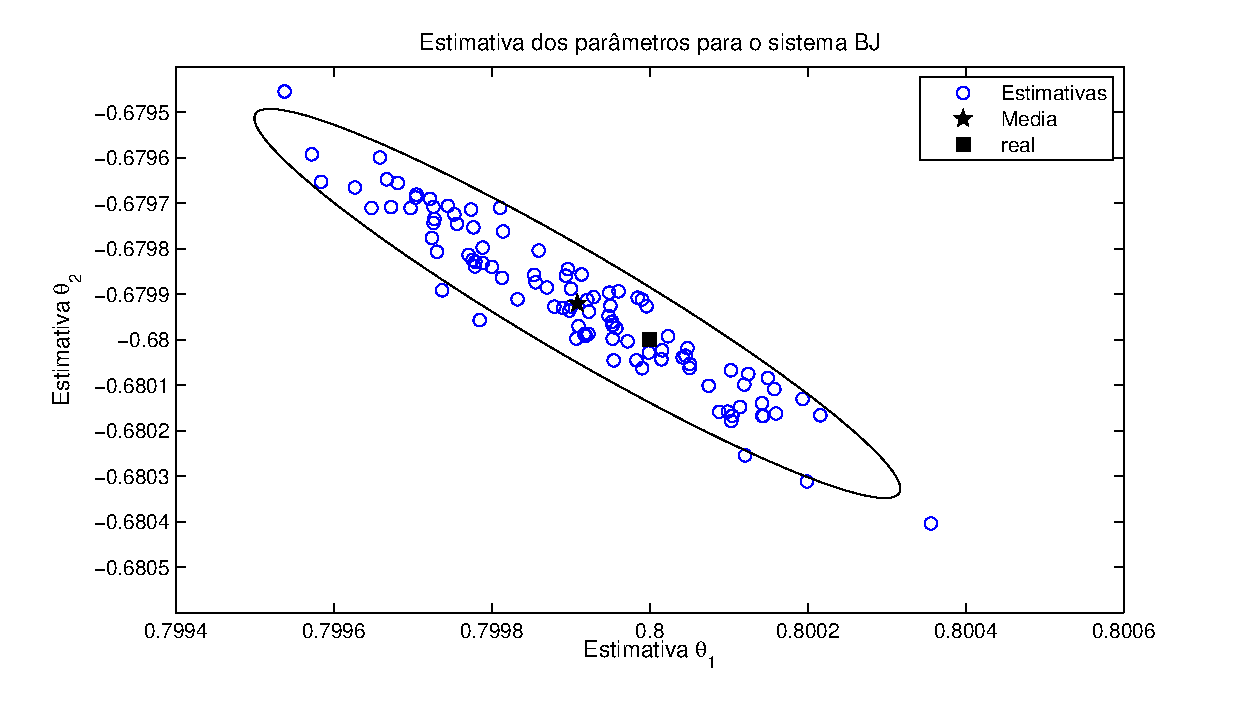
\includegraphics[width=0.95\columnwidth]{figures/vrft_bj_M10_var005.eps}
	\caption{Resultado das 100 estimativas de Monte Carlo dos par�metros $\theta_1$ e $\theta_2$ para o controlador
	apresentado em \eqref{eq:vrft_methos_ex_bj_c}. Adicionado a simula��o um ru�do aditivo de vari�ncia $\sigma_e^2=0.005$}
	\label{fig:vrft_bj_M10_var005}
\end{figure}

Os par�metros reais esperados para o controlador (equa��o \eqref{eq:vrft_methos_ex_bj_cd}) e a m�dia de todas
as estimativas $\hat{\theta}_N$ (valor representado por uma estrela na Figura (\ref{fig:vrft_bj_M10_var005})) n�o s�o os
mesmos. Em uma situa��o onde o erro de polariza��o das estimativas n�o existe, o aumento de N (n�mero de
amostras) implica que esta diferen�a diminui, tendendo a zero. Em um cen�rio onde h� erro de polariza��o, se 
aumentarmos a vari�ncia do ru�do do sistema, ser� observado um aumento desta diferen�a.

\begin{equation}
\lim_{N \rightarrow \infty }\hat{\theta}_N = \theta_0
\nonumber
\end{equation}

Na figura (\ref{fig:vrft_bj_M10_var02})  � apresentado o resultado para a estimativa de $\theta$ quando a vari�ncia do 
ru�do � quadruplicada ($\sigma_e^2=0.02$). Observa-se ent�o que o erro de polariza��o existe na estimativa. Como
descrito em \cite{campi_leccini_savaresi2002} quando o m�todo do VRFT � utilizado com ru�do nas amostras, a estimativa
� inevitavelmente polarizada. Na se��o (\ref{sec:dbcd_vrft_framework_noise}) foi sugerido o uso de vari�veis
instrumentais par para que este erro de polariza��o seja minimizado. Utilizou-se ent�o este m�todo e para um ru�do com
a mesma vari�ncia ($\sigma_e ^2=0.02$), o resultado �btido � o apresentado na Figura (\ref{fig:vrft_bj_M10_var02_iv}).

\begin{figure}[htbp] 
	\center 
	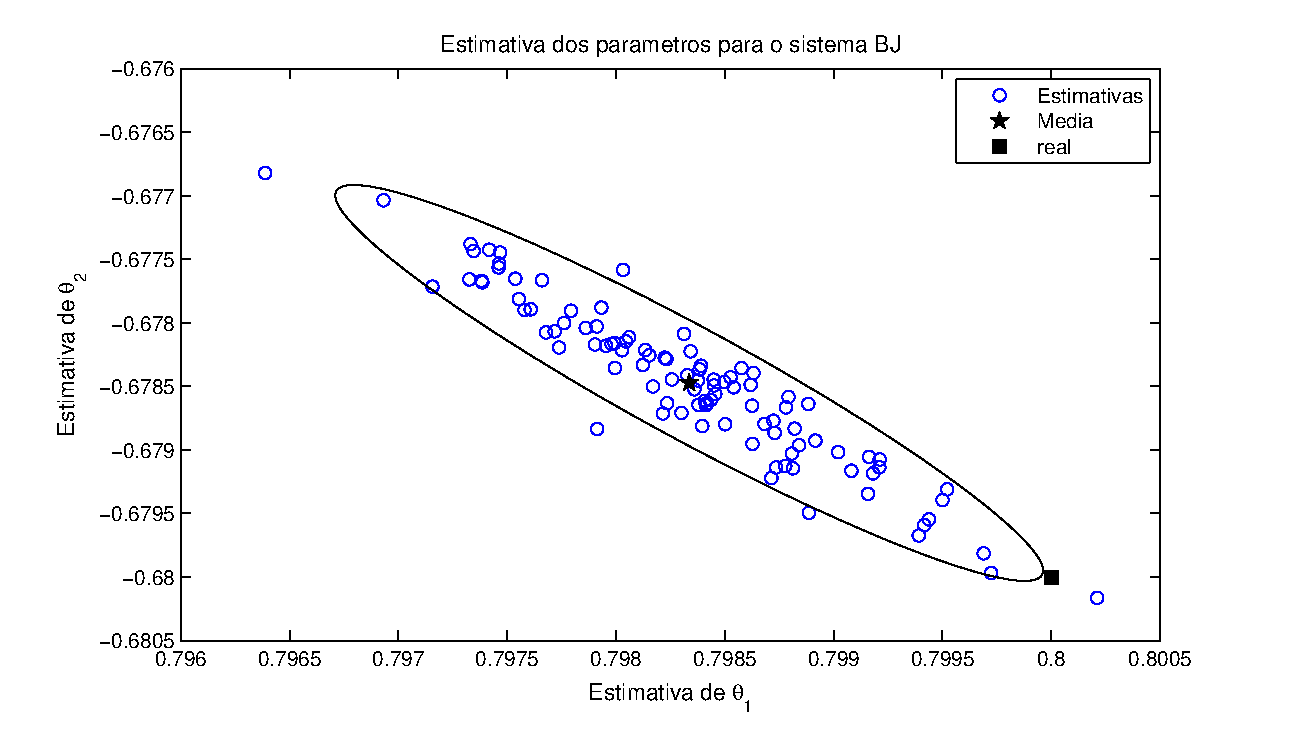
\includegraphics[width=0.95\columnwidth]{figures/vrft_bj_M10_var02.eps}
	\caption{100 estimativas Monte Carlo dos par�metros $\theta_1$ e $\theta_2$ para o controlador apresentado em
	\eqref{eq:vrft_methos_ex_bj_c} com um ru�do de vari�ncia de $\sigma_e^2=0.02$.}
	\label{fig:vrft_bj_M10_var02}
\end{figure}

\begin{figure}[htbp]
	\center
	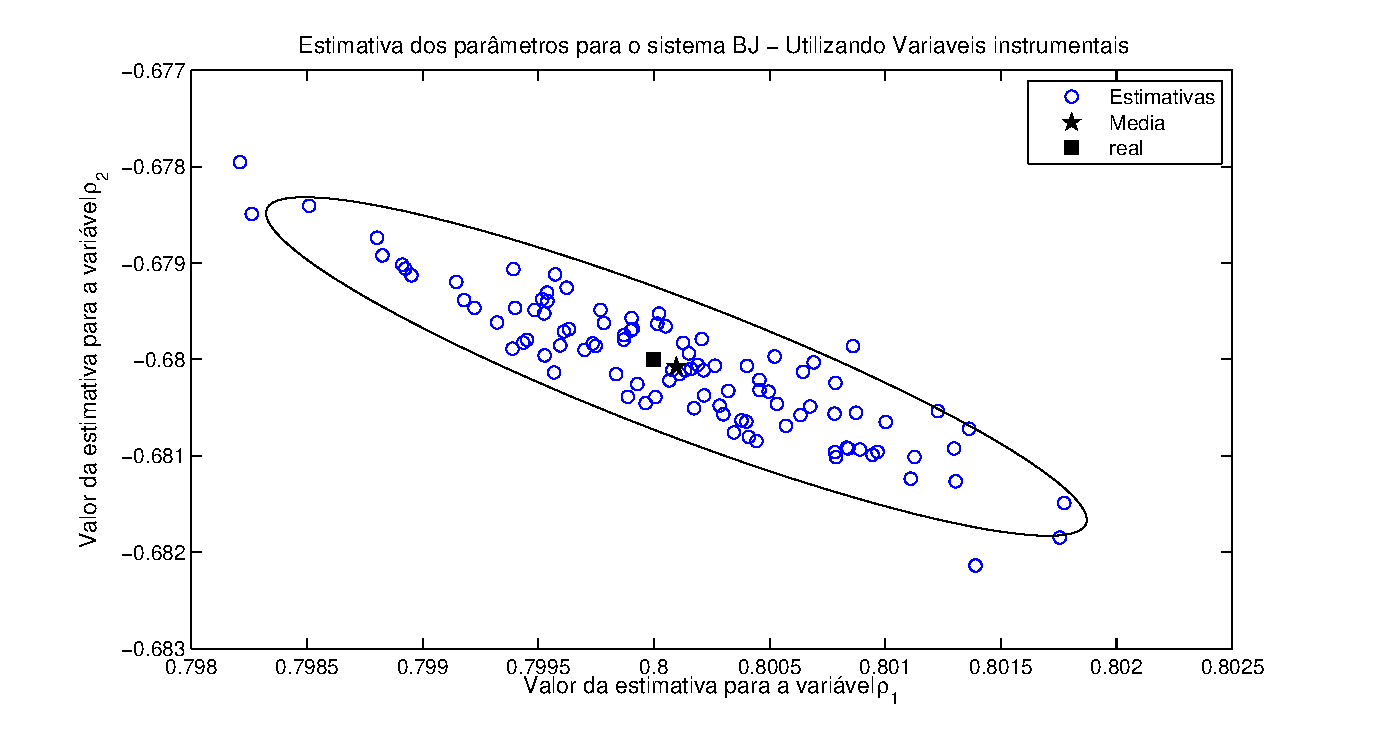
\includegraphics[width=0.95\columnwidth]{figures/vrft_bj_M10_var02_iv.eps}
	\caption{Resultado das 100 estimativas de Monte Carlo dos par�metros $\theta_1$ e $\theta_2$ para o
	controlador apresentado em \eqref{eq:vrft_methos_ex_bj_c} com vari�ncia do
	ru�do de 0.02. Utilizando vari�veis instrumentais para estimar os par�metros.}
	\label{fig:vrft_bj_M10_var02_iv}
\end{figure}

Observa-se que o erro de polariza��o foi minimizado e que o resultado obtido possui um custo $J_{VR}^N(\theta)
= 5.1242$ e a vari�ncia dos par�metros estimados foi de $0.5064\times10^{-6}$ para $\theta_1$ e de
$0.5495\times10^{-6}$ para $\theta_2$.

A fim de comparar o m�todo VRFT utilizando e n�o utilizando vari�veis instrumentais s�o apresentados abaixo as
Tabelas (\ref{table:vrft_method_bj}) e (\ref{table:vrft_method_bj_iv}) onde os custo $J_{y}$ e $J_{VR}^N$ s�o
apresentados para diferentes valores de vari�ncia do ru�do para o mesmo sistema BJ.

\begin{table*}[htbp]
\begin{center}
\caption{Valor dos custos $J_{VR}^N$ e $J_{y}$ al�m da vari�ncia das estimativas para diferentes valores de $\sigma_e^2$
quando o m�todo VRFT n�o utiliza vari�veis instrumentais para a estimativa dos par�metros $\theta$}
\label{table:vrft_method_bj}
\begin{tabular}{ccccc}
\hline
        Vari�ncia $\sigma_e^2$ & $J_{VR}^N(\theta)$ & $J_y(\theta)$ & M�dia $\theta_1$ & M�dia $\theta_2$  \\
\hline
	 0.1 	 & 	 4.87826e-02 	 & 	 2.15324e-02 	 & 	 0.76178 	 & 	 0.64466 \\ 
	 0.08 	 & 	 3.26789e-02 	 & 	 1.35688e-02 	 & 	 0.7759 	 & 	 0.65765 \\ 
	 0.06 	 & 	 1.80426e-02 	 & 	 7.86422e-03 	 & 	 0.78597 	 & 	 0.66715 \\ 
	 0.05 	 & 	 1.19341e-02 	 & 	 5.52796e-03 	 & 	 0.79017 	 & 	 0.67088 \\ 
	 0.04 	 & 	 7.54289e-03 	 & 	 3.65088e-03 	 & 	 0.79351 	 & 	 0.67396 \\ 
	 0.01 	 & 	 4.89481e-04 	 & 	 2.11052e-04 	 & 	 0.79962 	 & 	 0.67965 \\ 
	 0.008 	 & 	 3.25810e-04 	 & 	 1.83444e-04 	 & 	 0.79968 	 & 	 0.67969 \\ 
	 0.005 	 & 	 1.20816e-04 	 & 	 5.42193e-05 	 & 	 0.7999 	 & 	 0.67991 \\ 
	 0.003 	 & 	 4.73517e-05 	 & 	 2.28052e-05 	 & 	 0.79996 	 & 	 0.67996 \\ 
	 0.001 	 & 	 5.02347e-06 	 & 	 2.77267e-06 	 & 	 0.8 	     & 	 0.68 \\ 
\hline
\end{tabular}
\end{center}
\end{table*} 
   

\begin{table*}[htbp]
\begin{center}
\caption{Valor dos custos $J_{VR}^N$ e $J_{y}$ al�m da  vari�ncia das estimativas para diferentes valores de
$\sigma_e^2$ quando o m�todo VRFT utiliza vari�veis instrumentais para a estimativa dos par�metros $\theta$}
\label{table:vrft_method_bj_iv}
\begin{tabular}{ccccc}
\hline
        Vari�ncia $\sigma_e^2$ & $J_{VR}^N(\theta)$ & $J_{y}(\theta)$  & M�dia $\theta_1$ & M�dia $\theta_2$  \\
\hline
	 0.1 	 & 	 5.19132e-02 	 & 	 4.14964e-04 	 & 	 0.79936 	 & 	 0.67971 \\ 
	 0.08 	 & 	 3.31577e-02 	 & 	 2.96000e-04 	 & 	 0.80037 	 & 	 0.68007 \\ 
	 0.06 	 & 	 1.70932e-02 	 & 	 2.17256e-04 	 & 	 0.79989 	 & 	 0.67969 \\ 
	 0.05 	 & 	 1.27803e-02 	 & 	 3.14017e-05 	 & 	 0.80006 	 & 	 0.68005 \\ 
	 0.04 	 & 	 7.72145e-03 	 & 	 9.43578e-05 	 & 	 0.79996 	 & 	 0.68006 \\ 
	 0.01 	 & 	 5.00316e-04 	 & 	 3.20694e-05 	 & 	 0.80005 	 & 	 0.68003 \\ 
	 0.008 	 & 	 3.44326e-04 	 & 	 2.93508e-05 	 & 	 0.80001 	 & 	 0.68004 \\ 
	 0.005 	 & 	 1.19855e-04 	 & 	 6.96916e-06 	 & 	 0.79999 	 & 	 0.68 \\ 
	 0.003 	 & 	 4.22380e-05 	 & 	 6.33696e-06 	 & 	 0.80001 	 & 	 0.68001 \\ 
	 0.001 	 & 	 5.08709e-06 	 & 	 1.18016e-06 	 & 	 0.8 	 	 & 	 0.68 \\ 
\hline
\end{tabular}
\end{center}
\end{table*}

Utilizando vari�veis instrumentais observa-se que o custo $J_{y}(\theta)$ � significativamente mais baixo
quando comparado com o m�todo onde n�o s�o utilizadas vari�veis instrumentais, corroborando com o que foi apresentado na
se��o (\ref{sec:dbcd_vrft_framework_noise}).

%===============================================================================
\subsubsection{Controlador PID - sistema ARX}
\label{sec:dbcd_vrft_examples_pid_arx}
%===============================================================================

Considere o sistema real definido pefinido pelo modelo ARX:

\begin{equation}
G_{ 0 }(z)=\frac { z }{ (z-0.9)(z-0.8) } ,\quad \quad \quad H_{ 0 }(z)=\frac { z^2 }{ (z-0.9)(z-0.8) } 
\nonumber
\end{equation}

Deseja-se que o sistema em malha fechada comporte-se como:

\begin{equation}
T_d(z)=\frac { 0.4 }{ z-0.6 }
\label{eq:vrft_methos_ex_arx_M}
\end{equation}

Tem-se assim que o controlador ideal � definido por:

\begin{equation}
C_d(z)=\frac{T_d(z)}{G_0(z)(1-T_d(z))}=\frac { 0.4(z - 0.9)(z-0.8) }{ z(z-1) }
\label{eq:vrft_methos_ex_arx_cd}
\end{equation}

Observa-se que este controlador pode ser representado como um controlador
{\it{PID}} como em: 

\begin{equation}
C(z,\theta )=\frac { \theta _{ 1 }z^2+\theta _{ 2 }z+\theta _{ 3 } }{ z(z-1) } 
\label{eq:vrft_methos_ex_arx_c}
\end{equation}

Na Figura (\ref{fig:vrft_arx_M10_var005}) � apresentado o resultado da estimativa dos par�metros do
controlador quando n�o s�o utilizados vari�veis instrumentais. Juntamente com os valores das estimativas, � apresentado
o elips�ide de $\xi^2=95\%$ de confian�a. Obteve-se desta forma um custo $J_{VR}^N(\theta) = 2.5008\times10^{-5}$ e
$J_{y}(\theta) = 1.7746\times10^{-5}$ al�m de uma vari�ncia para as estimativas de $1.0\times10^{-7} \; [0.0364\;
0.1261\; 0.0377]$ para $\theta_1$, $\theta_2$ e $\theta_3$ respectivamente.

\begin{figure}[htbp] 
	\center 
	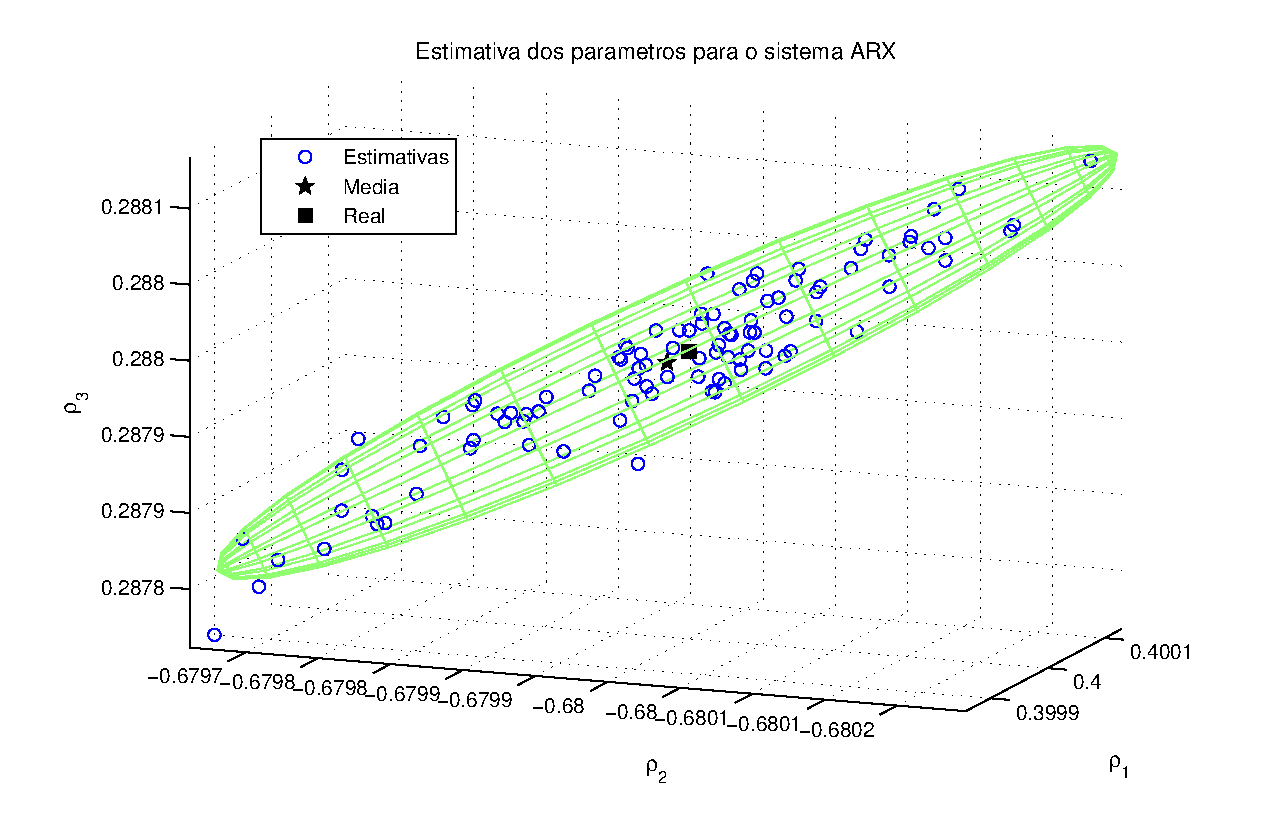
\includegraphics[width=0.95\columnwidth]{figures/vrft_arx_M10_var005_.eps}
	\caption{100 estimativas Monte Carlo dos par�metros $\theta_1$, $\theta_2$ e $\theta_3$ para o controlador
	apresentado em \eqref{eq:vrft_methos_ex_arx_c} com vari�ncia do ru�do $\sigma_e ^2=0.005$}
	\label{fig:vrft_arx_M10_var005}
\end{figure}

Como j� foi observado a utiliza��o de vari�veis instrumentais melhora significativamente o erro de polariza��o existente
nas estimativas do m�todo VRFT quaando h� presen�a de ru�do. Desta forma as informa��es apresentadas a seguir ser�o
feitas utilizando vari�veis instrumentais. Na figura (\ref{fig:vrft_arx_M10_var05_iv}) � apresentado a estimativa dos
par�metros do controlador para um ru�do de vari�ncia $\sigma_e ^2=0.05$. Observa-se que n�o h� erro de polariza��o nas
estimativas. O custo para esta, e outas, estimativas � apresentado na Tabela (\ref{table:vrft_method_arx_iv}).

\begin{figure}[htbp] 
	\center 
	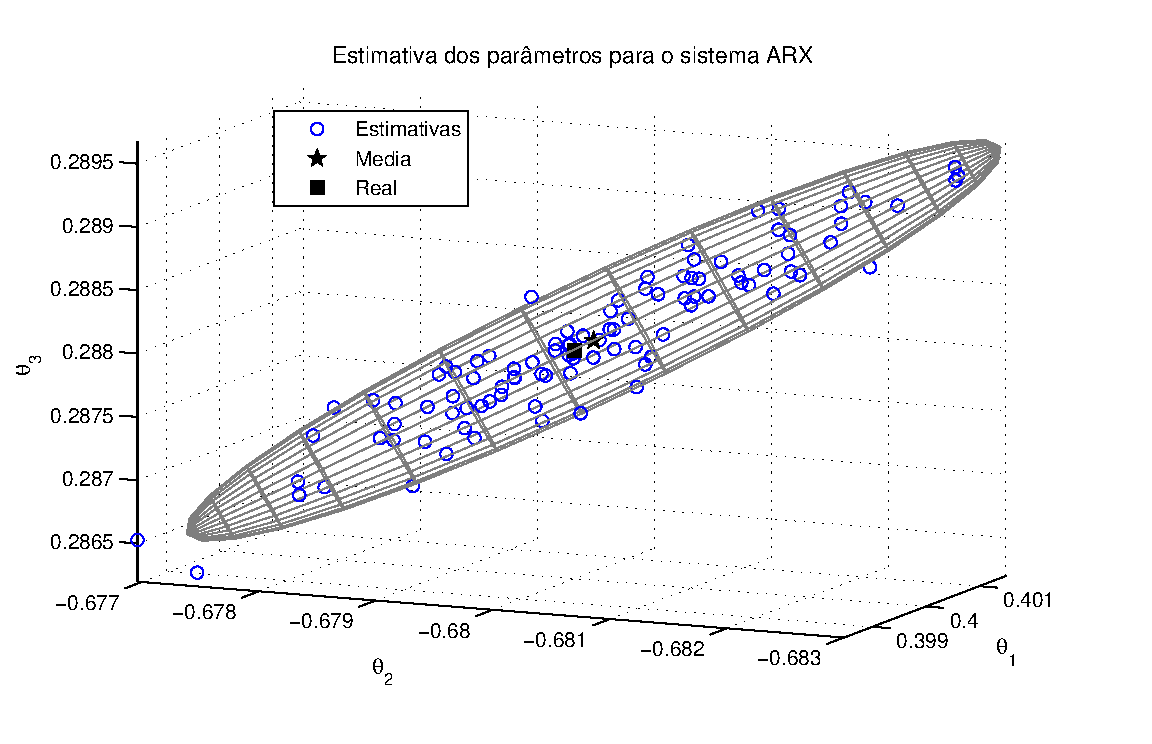
\includegraphics[width=0.95\columnwidth]{figures/vrft_arx_M10_var05_iv.eps}
	\caption{100 estimativas Monte Carlo dos par�metros $\theta_1$, $\theta_2$ e $\theta_3$ para o controlador
	apresentado em \eqref{eq:vrft_methos_ex_arx_c} com vari�ncia do ru�do $\sigma_e ^2=0.05$ utilizando
	vari�veis instrumentais}
	\label{fig:vrft_arx_M10_var05_iv}
\end{figure}


\begin{table*}[htbp]
\begin{center}
\caption{Valor dos custos $J_{VR}^N$ e $J_{y}$ al�m da  vari�ncia das
estimativas para diferentes valores de $\sigma_e^2$ quando o m�todo
VRFT utiliza vari�veis instrumentais para a estimativa dos par�metros $\theta$ do controlador
\eqref{eq:vrft_methos_ex_arx_c}}
\label{table:vrft_method_arx_iv}
\begin{tabular}{cccc}
\hline
        Vari�ncia $\sigma_e^2$ & $J_{VR}^N(\theta)$ &
        $J_{y}(\theta)$ & Vari�ncia estimativas $\theta$   \\
\hline
   0.1     & $10.0743\times10^{-3}$ &  2.2871$\times10^{-3}$ & $1\times10^{-5}\;[0.1253 \; 0.4683 \; 0.1600]$ \\
   0.06    & $ 3.6093\times10^{-3}$ &  1.1279$\times10^{-3}$ & $1\times10^{-5}\;[0.0516 \; 0.1793 \; 0.0575]$ \\
   0.05    & $ 2.5419\times10^{-3}$ &  1.2453$\times10^{-3}$ & $1\times10^{-5}\;[0.0344 \; 0.1237 \; 0.0416]$ \\
   0.04    & $ 1.6013\times10^{-3}$ &  0.5106$\times10^{-3}$ & $1\times10^{-6}\;[0.2195 \; 0.7908 \; 0.2379]$ \\
   0.01    & $10.0077\times10^{-5}$ & 13.7142$\times10^{-5}$ & $1\times10^{-7}\;[0.1552 \; 0.5469 \; 0.1822]$ \\
   0.005   & $ 2.5081\times10^{-5}$ & 10.3482$\times10^{-5}$ & $1\times10^{-7}\;[0.0406 \; 0.1260 \; 0.0375]$ \\
	0.001  & $ 0.1009\times10^{-5}$ &  2.0487$\times10^{-5}$ & $1\times10^{-9}\;[0.1277 \; 0.4035 \;0.1239]$	 \\
\hline
\end{tabular}
\end{center}
\end{table*}

%===============================================================================
\subsubsection{Controlador n�o pertence a classe}
\label{sec:dbcd_vrft_examples_not_in_class}
%===============================================================================

At� este ponto foram apresentados exemplos de uso do m�todo VRFT quando o controlador que leva o sistema para
o comportamento desejado $T_d(z)$ faz parte da classe escolhida para a identifica��o. Nesta se��o ser� apresentado um
exemplo onde a classe de modelos do controlador escolhida n�o consegue represetar o controlador ideal $C_d(z)$.

Considerando o sistema real descrito por:

\begin{equation}
G_{ 0 }(z)=\frac { 0.2(z-0.7) }{ (z-0.9)(z-0.5) } ,\quad \quad \quad H_{ 0 }(z)=\frac { z }{ z-0.3 } 
\nonumber
\end{equation}

Deseja-se que em malha fechada ele se comporte como em: 

\begin{equation}
T_d(z)=\frac { 0.16z }{ (z-0.6)^2 }
\label{eq:vrft_methos_ex_pid_not_M}
\end{equation}

Neste caso o controlador ideal � definido por

\begin{equation}
C_{ d }(z)=\frac { 0.8z(z-0.9)(z-0.5) }{ (z-1)(z-0.36)(z-0.7) } 
\label{eq:vrft_methos_ex_pid_not_cd}
\end{equation}

Para esta identifica��o optou-se por um controlador do tipo PID como em:
 
\begin{equation}
C(z,\theta )=\frac { \theta _{ 1 }z^2+\theta _{ 2 }z+\theta _{ 3 } }{ z(z-1) } 
\label{eq:vrft_methos_ex_pid_not_c}
\end{equation}

Observa-se que \eqref{eq:vrft_methos_ex_pid_not_c} n�o consegue representar todas as din�micas apresentadas em
\eqref{eq:vrft_methos_ex_pid_not_cd}. Utilizando o procedimento descrito na Se��o
(\ref{sec:dbcd_vrft_framework_noise}) e o procedimento de experimento repetido, foram feitos 100 experimentos de
Monte Carlo e o resultado obtido para a m�dia das estimativas foi:

\begin{equation}
\theta_L =\left[ 0.8101 \quad -0.1691  \quad -0.3358 \right]
\nonumber
\end{equation}

onde o �ndice $L$ indica que este resultado foi obtido utilizando-se o filtro $L$.

Repetindo a simula��o, mas agora sem que o procedimento da utiliza��o do filtro $L$ descrito na se��o
(\ref{sec:dbcd_vrft_framework_noise}), obteve-se o resultado seguinte:

\begin{equation}
\theta =\left[ 0.5846 \quad -0.2108  \quad -0.1525 \right]
\nonumber
\end{equation}

Aplicando-se estes resultados ao controlador apresentado em \eqref{eq:vrft_methos_ex_pid_not_c} e de posse do
comportamento desejado para o sistema em malha fechada ($T_d(z)$) � poss�vel fazer um comparativo da resposta
ao salto unit�rio para o sistema utilizando os dois controladores obtidos. O resultado � apresentado na Figura
(\ref{fig:vrft_notinclass_step}).

\begin{figure}[htbp] 
	\center 
	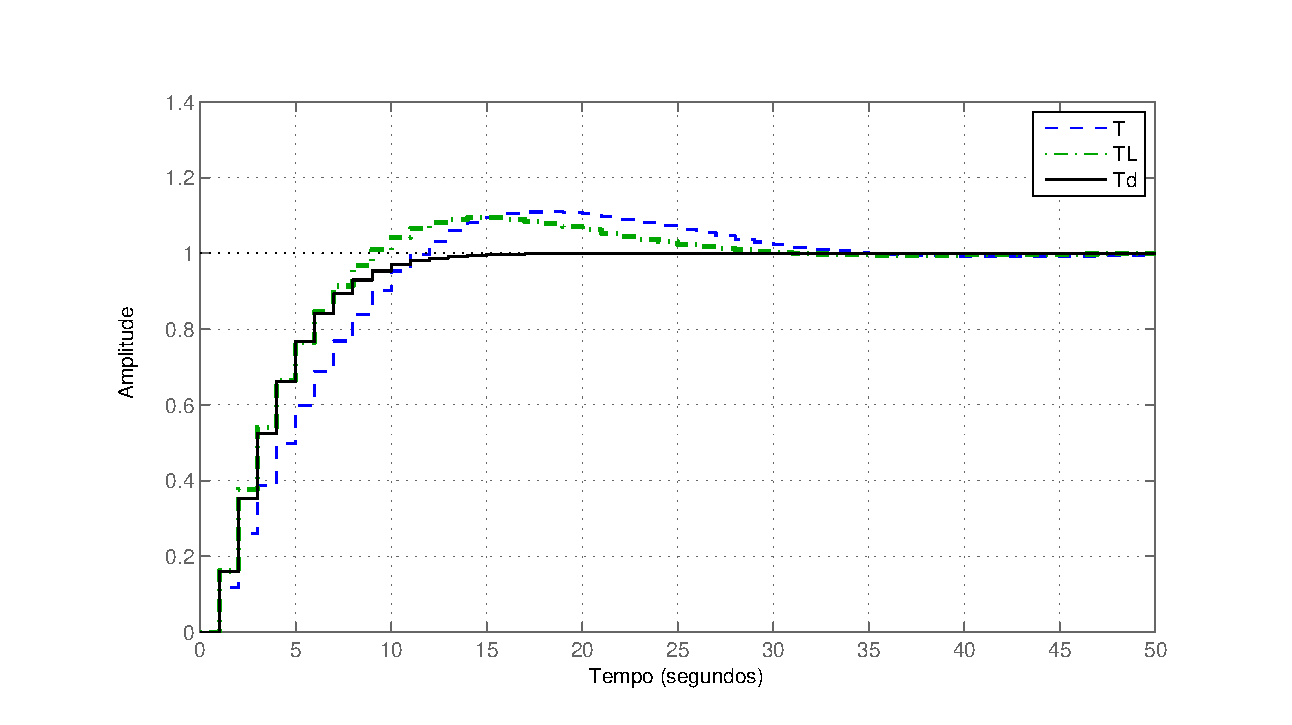
\includegraphics[width=0.85\columnwidth]{figures/vrft_notinclass_step.eps}
	\caption{Comparativo da resposta do sistema a um degrau unit�rio quando o controlador inserido � obtido pelo
	m�todo VRFT utilizando o filtro L e quando n�o se utiliza este artificio. O sistema foi simulado com um
	ru�do de vari�ncia $\sigma_e ^2=0.1$}
	\label{fig:vrft_notinclass_step}
\end{figure}

Observa-se que para o sistema que utiliza o controlador estimado utilizando-se o filtro $L$, a resposta ao
degrau unit�rio tem significativamente menos erro que o sistema utilizando o outro controlador. Ficando este
primeiro muito mais pr�ximo da fun��o $T_d(z)$ desejada.

Os custos destes dois sistemas � apresentado na Tabela (\ref{table:vrft_method_notinclass}).

\begin{table*}[htbp]
\begin{center}
\caption{Valor dos custos $J_{VR}^N$ e $J_{y}$ para o sistema controlado por $C(z)$ e $C_L(z)$}
\label{table:vrft_method_notinclass}
\begin{tabular}{ccc}
\hline
        Controlador & $J_{VR}^N(\theta)$ & $J_{y}(\theta)$ \\
\hline
	$C(z)$   & 0.2877 &  0.1270 \\
	$C_L(z)$ & 0.4481 &  0.0542 \\
\hline
\end{tabular}
\end{center}
\end{table*}

A fim de comparar as duas estimativas, na figura (\ref{fig:vrft_notinclass_bode}) � apresentado o diagrama de
Bode dos controladores obtidos (utilizando a m�dia das estimativas obtidas).

\begin{figure}[htbp] 
	\center 
	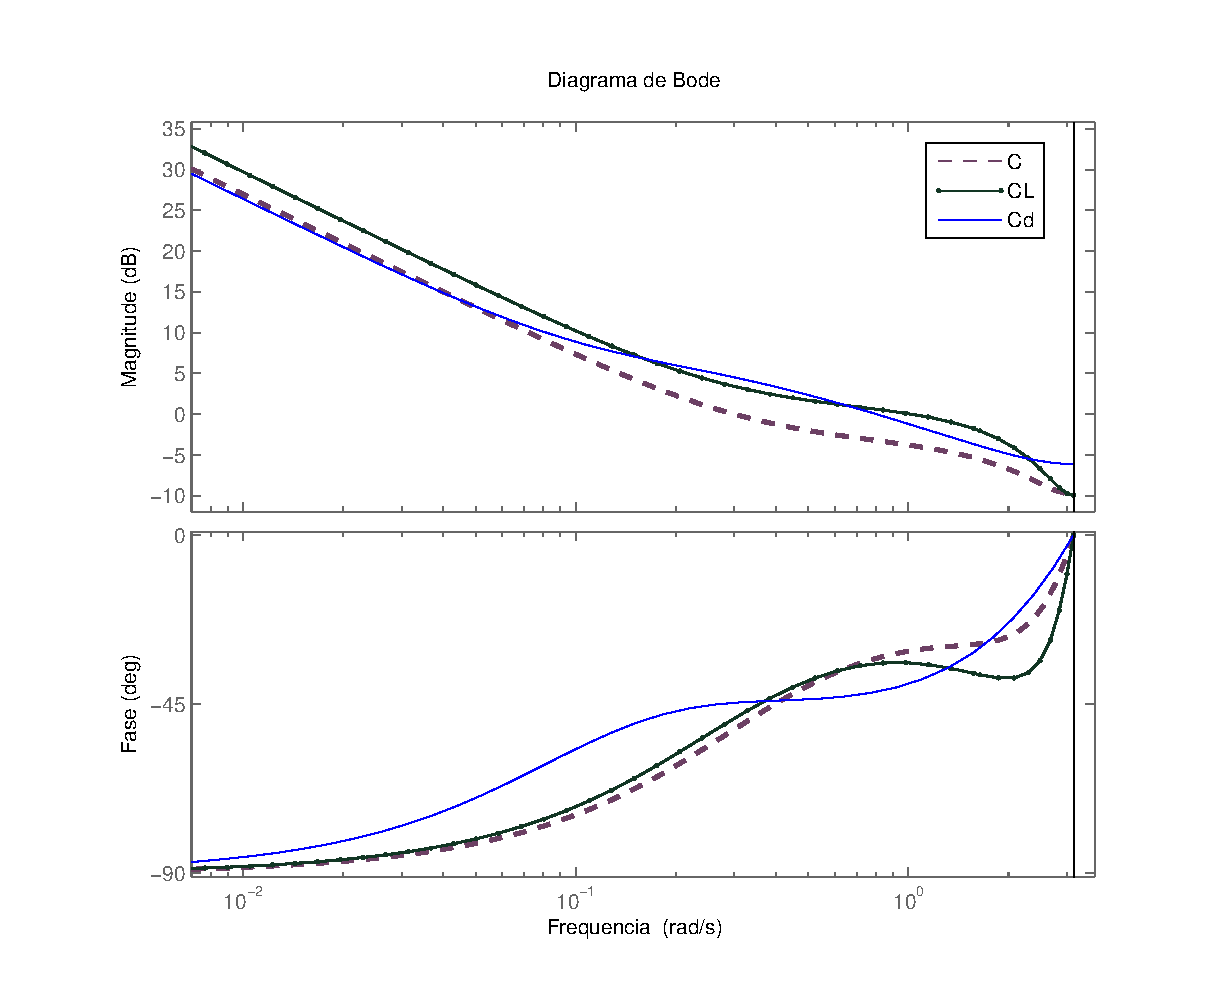
\includegraphics[width=0.85\columnwidth]{figures/vrft_notinclass_bode.eps}
	\caption{Diagrama de Bode para as fun��es de transfer�ncia dos controladores estimados utilizando VRFT com e
	sem o artificio do filtro L e vari�veis instrumentais}
	\label{fig:vrft_notinclass_bode}
\end{figure}


%===============================================================================
\section{Considera��es Finais}
\label{sec:dbcd_conclusions}
%===============================================================================


%===============================================================================


%===============================================================================
\chapter{Identifica��o de sistemas n�o lineares utilizando refer�ncia virtual}
\label{chapter:dbnarmax}
%===============================================================================
Na se��o \ref{sec:dbnarmax_nonlinear} introduz-se a id�ia de utiliza��o de m�todos de projeto de controladores baseados
em dados, juntamente com a utilzia��o de refer�ncia virtual para a obten��o dos sinais necess�rios. Esta se��o utiliza o
algoritmo apresentado na se��o \ref{sec:nl_si_algorithms_rationals} para identifica��o de sistemas n�o lineares que
podem ser descritos por classes de modelos NARMAX polinomiais ou racionais. Alguns exemplos ser�o apresentados para que
se possa avaliar a qualidade das estimativas obtidas.

%===============================================================================
% ===============================================================================
\section{Identifica��o de controladores n�o lineares utilizando refer�ncia virtual}
\label{sec:dbnarmax_nonlinear}
%===============================================================================

\cite{Guardabassi}

Em \cite{campi_savaresi2006} foi apresentado uma generaliza��o do m�todo VRFT para sistemas n�o lineares, existe
entretanto a necessidade de um filtro dependente dos dados coletados do sistema e derivar esta informa��o com base nos
dados de entrada. O filtro em quest�o tem o formato:

\begin{equation}
F=(I-MD) \left ( \frac{\partial G\left [ u \right ]}{\partial u}|_{\tilde{u}} \right ) 
\label{eq:vrft_nl_filter}
\end{equation} 

Como obter o valor de $ \frac{\partial G\left [ u \right ]}{\partial u}$ � bastatne custoso e requer bom conhecimento
dos dados de entrada da planta, optou-se por utilizar uma abordagem diferente da sugerida em
\cite{campi_savaresi2006}.

Mant�m-se a id�ia do m�todo VRFT para a obten��o dos sinais de entrada do controlador. De posse destes sinais e dos
sinais utilizados para excitar a planta, � poss�vel utilizar outros algoritmos de identifica��o de sistemas n�o lineares
para determinar o ajuste dos parametros da estrutura do controlador n�o linear escolhido {\it{a priori}}.

% ===============================================================================
\subsection{Identifica��o de controladores representados por classes NARMAX}
\label{sec:dbnarmax_nonlinear_narmax}
%===============================================================================

De posse dos dados de entrada e sa�da do controlador, obtidos por meio da utiliza��o de refer�ncia virtual, optou-se por
utilizar o algoritmo proposto na se��o \ref{sec:nl_si_algorithms_rationals} para ajustar os parametros do controlador
n�o linear caracterizado por uma classe de modelos NARMAX. Este algoritmo mostrou-se bastante eficiente para
identifica��o de sistemas NARMAX, racionais e polinomiais. Al�m do mais, estas fam�lias de modelos s�o capazes de
representar uma grande variedade de sistemas n�o lineares.

Neste trabalho focou-se na identifica��o de controladores caracterizados por modelos NARMAX, mas a id�ia do uso de
refer�ncia virtual em conjunto com algoritmos idependentes para identifica��o de sistemas n�o lineares, pode ser
facilmente expandida, se assim for conveninte.















%===============================================================================
\section{Considera��es Finais}
\label{sec:dbnarmax_conclusions}
%===============================================================================

Neste cap�tulo apresentou-se a uni�o das ideias de utiliza��o de refer�ncia virtual para a obten��o dos sinais
necess�rios para a determina��o do controlador �timo e a ideia de utiliza��o de algoritmos de identifica��o de sistemas
n�o lineares para determina��o do controlador �timo quando este faz parte de uma classe de modelos n�o linear.

Descreveu-se inicialmente a ideia generalizada onde a classe de modelos n�o linear do controlador precisa estar atrelada
apenas ao algoritmo utilizado para sua identifica��o. Devido aos bons resultados obtidos com a identifica��o de sistemas
NARMAX apresentados no Ccap�tulo \ref{chapter:nlin_si_ident}, optou-se por utilizar este algoritmo (Se��o
\ref{sec:nl_si_algorithms_rationals}) para determinar os par�metros do controlador utilizando-se para isso entretanto
dos sinais obtidos por meio do m�todo de refer�ncia virtual.

Na Se��o \ref{sec:dbnarmax_nonlinear_examples} apresentou-se alguns exemplos para demonstrar a viabilidade da utiliza��o
da metodologia. Foram apresentados exemplos onde a classe de modelos consegue representar a totalidade das din�micas de
$C_d(z)$ para que o sistema se comporte em malha fechada linearmente como escolhido por $T_d(z)$. Outro exemplo foi
apresentado quando n�o existe uma completa descri��o do controlador ideal pela classe de modelos, ou seja, $C_d(z)
\notin C(z, \theta)$, apresentou-se um comparativo do sistema ideal e do obtido utilizando o controlador obtido quando o
sistema � submetido a um degrau unit�rio.

Tamb�m foi apresentado um exemplo onde o controlador � descrito por um modelo NARMAX polinomial, em um contexto onde a
planta do sistema possui uma n�o linearidade est�tica na sa�da do processo, caso este onde o controlador ideal tamb�m
n�o se encontra na classe de modelos. A aproxima��o do modelo escolhido para este controlador se mostrou relativamente
pr�ximo ao controlador ideal, visto que o cancelamento da n�o linearidade da planta foi quase completo, como apresentado
na Figura \ref{fig:vrft_nl_wiener_vw}.

De forma geral, apresentou-se neste cap�tulo a utiliza��o desta metodologia de identifica��o de controladores n�o
lineares descritos por modelos NARMAX, polinomial ou racional e seus resultados. Os resultados obtidos mostram que a
metodologia � v�lida e que em situa��es onde o controlador ideal pode ser bem representado pela classe de controladores,
os resultados obtidos n�o possuem erro de polariza��o para experimentos executados em malha aberta. O estudo para
experimentos em malha fechada n�o � escopo deste trabalho e pode ser encarado como um dos trabalhos futuros provenientes
desta pesquisa.

%===============================================================================

%===============================================================================
\section{Conclus�o}
\label{sec:conclusion}
%===============================================================================



% referencias
% Aqui pode ser usado o ambiente padrao `thebibliography'; por�m, fa�a um
% favor a s� mesmo e use o \bibtex\ e o estilo abnt.bst (veja na p�gina do
% UTUG). 

\bibliographystyle{abnt}

%\bibliography{exemplo,modelo} 	% pode-se ter v�rios arquivos .bib separados
\bibliography{neuhaus} 	% pode-se ter v�rios arquivos .bib separados
				% por v�rgulas. Segundo a NBR6023, as
				% refer�ncias devem ser alinhadas apenas a
				% esquerda. � esquisito, mas � assim.

% Ap�ndices
\appendix

%===============================================================================
% Pode-se ter diversos ap�ndices
\chapter{Algoritmo de identifica��o de sistemas n�o lineares}

Neste cap�tulo ser�o apresentados as rotinas criadas na ferramenta Matlab para a identifica��o de sistemas n�o lineares,
como descrito na Se��o \ref{sec:nl_si_algorithms_rationals}.

\lstinputlisting[language=Matlab,
				frame=box,
				label=lst:rational_model,
				caption=La�o principal do algoritmo implementado para identifica��o de
				sistemas n�o lineares descritos por modelos NARMAX]{code/functions/rational/f_rational_model.m}

\lstinputlisting[language=Matlab,
				frame=box,
				label=lst:rational_model,
				caption=La�o principal do algoritmo implementado para identifica��o de
				sistemas n�o lineares descritos por modelos NARMAX]{code/functions/rational/f_get_phy.m}
				


%
%
%% Anexos
%\annex
%
%% Pode-se ter diversos anexos
%\chapter{T�tulo do Anexo}
%
%J� os anexos ser�o textos, trabalhos e materiais que n�o foram elaborados
%pelo autor, mas que servem de comprova��o, fundamenta��o ou ilustra��o dos
%argumentos contidos no texto. Neste ponto, deve-se dar especial aten��o �
%quest�o dos direitos autorais.
%
\end{document}
